\section{NMR spectra}

\subsection{(\textit{S})-4-Bromo-\textit{N}-(2-oxotetrahydrofuran-3-yl)butanamide \compound{cmpd:HL4Br}}

\begin{figure}[H]
	\centering
		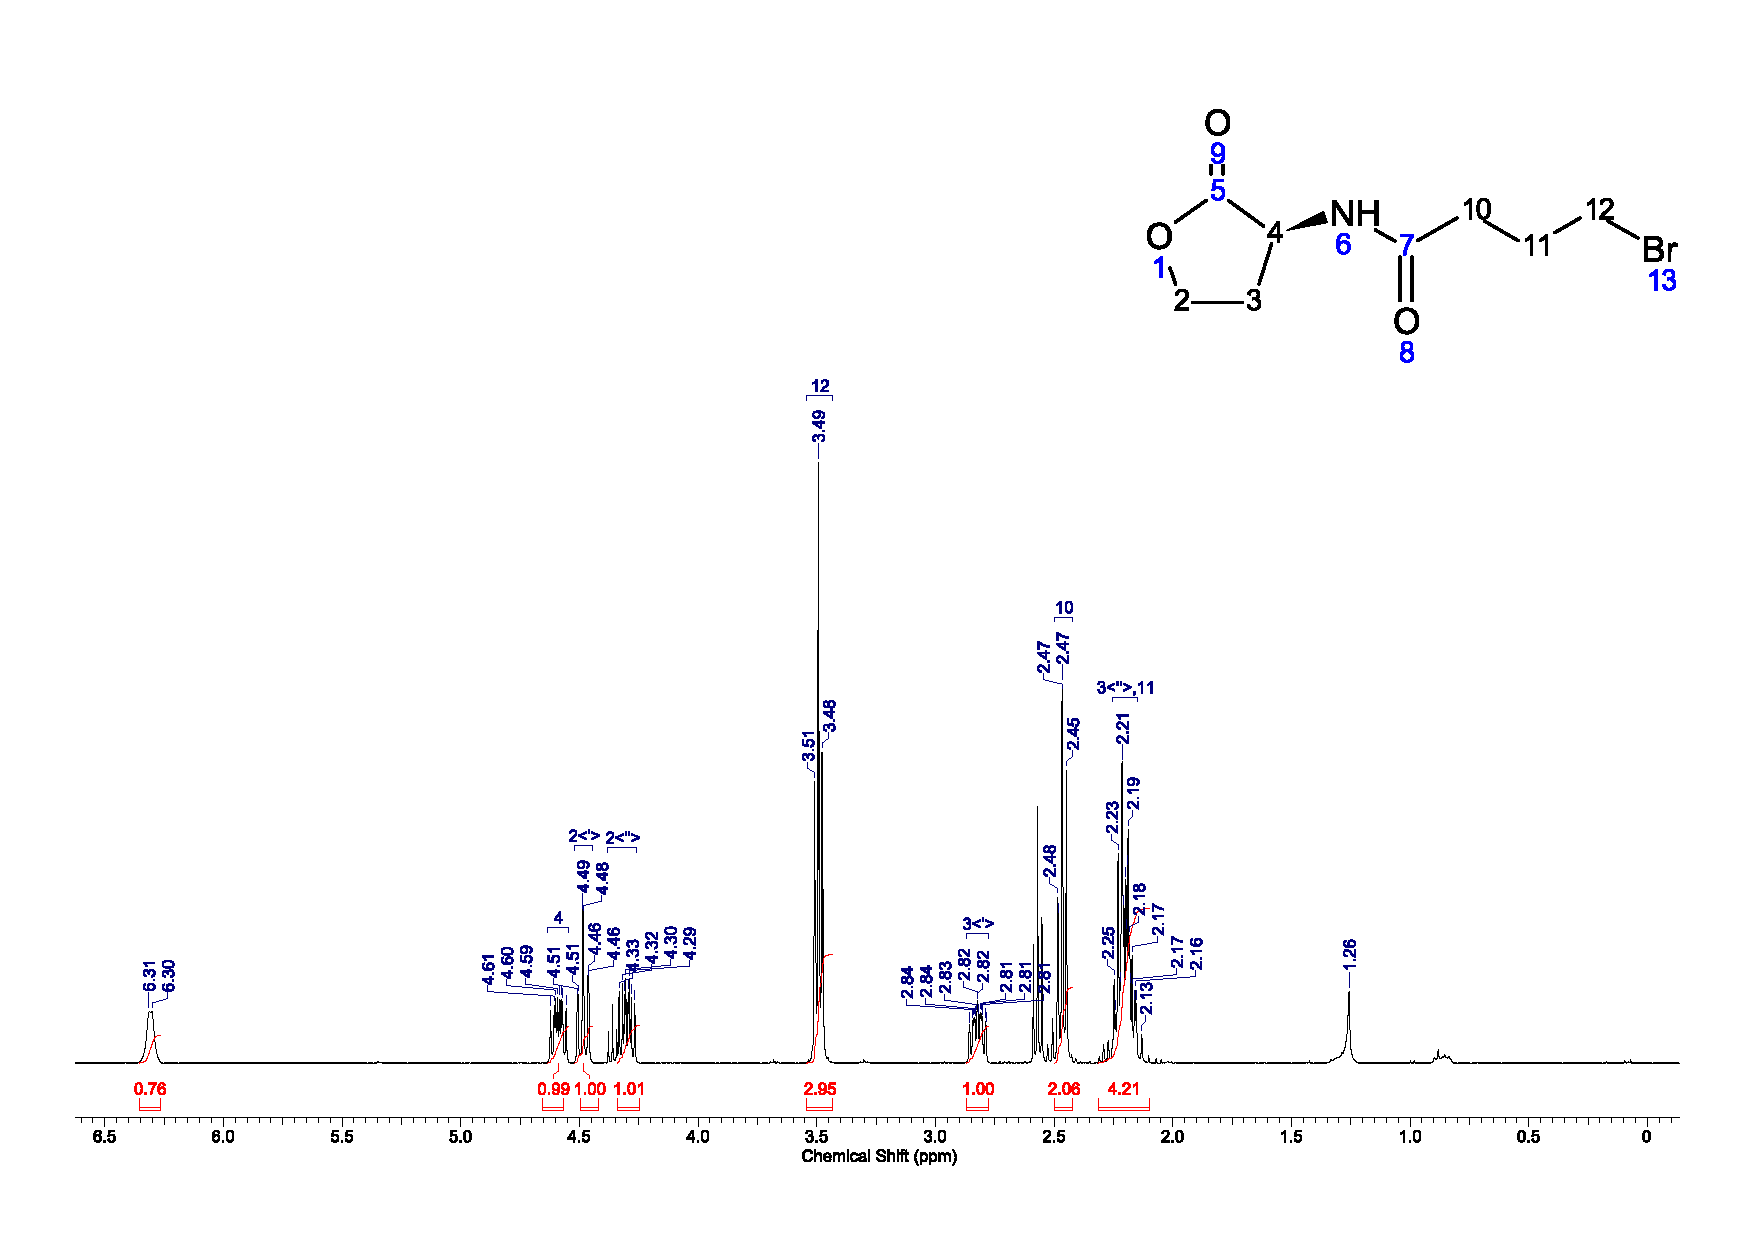
\includegraphics[ width=1.0\textwidth,height=0.43\textheight,keepaspectratio,trim={0 0 0 1.7cm},clip]{HL4Br_H.pdf}
		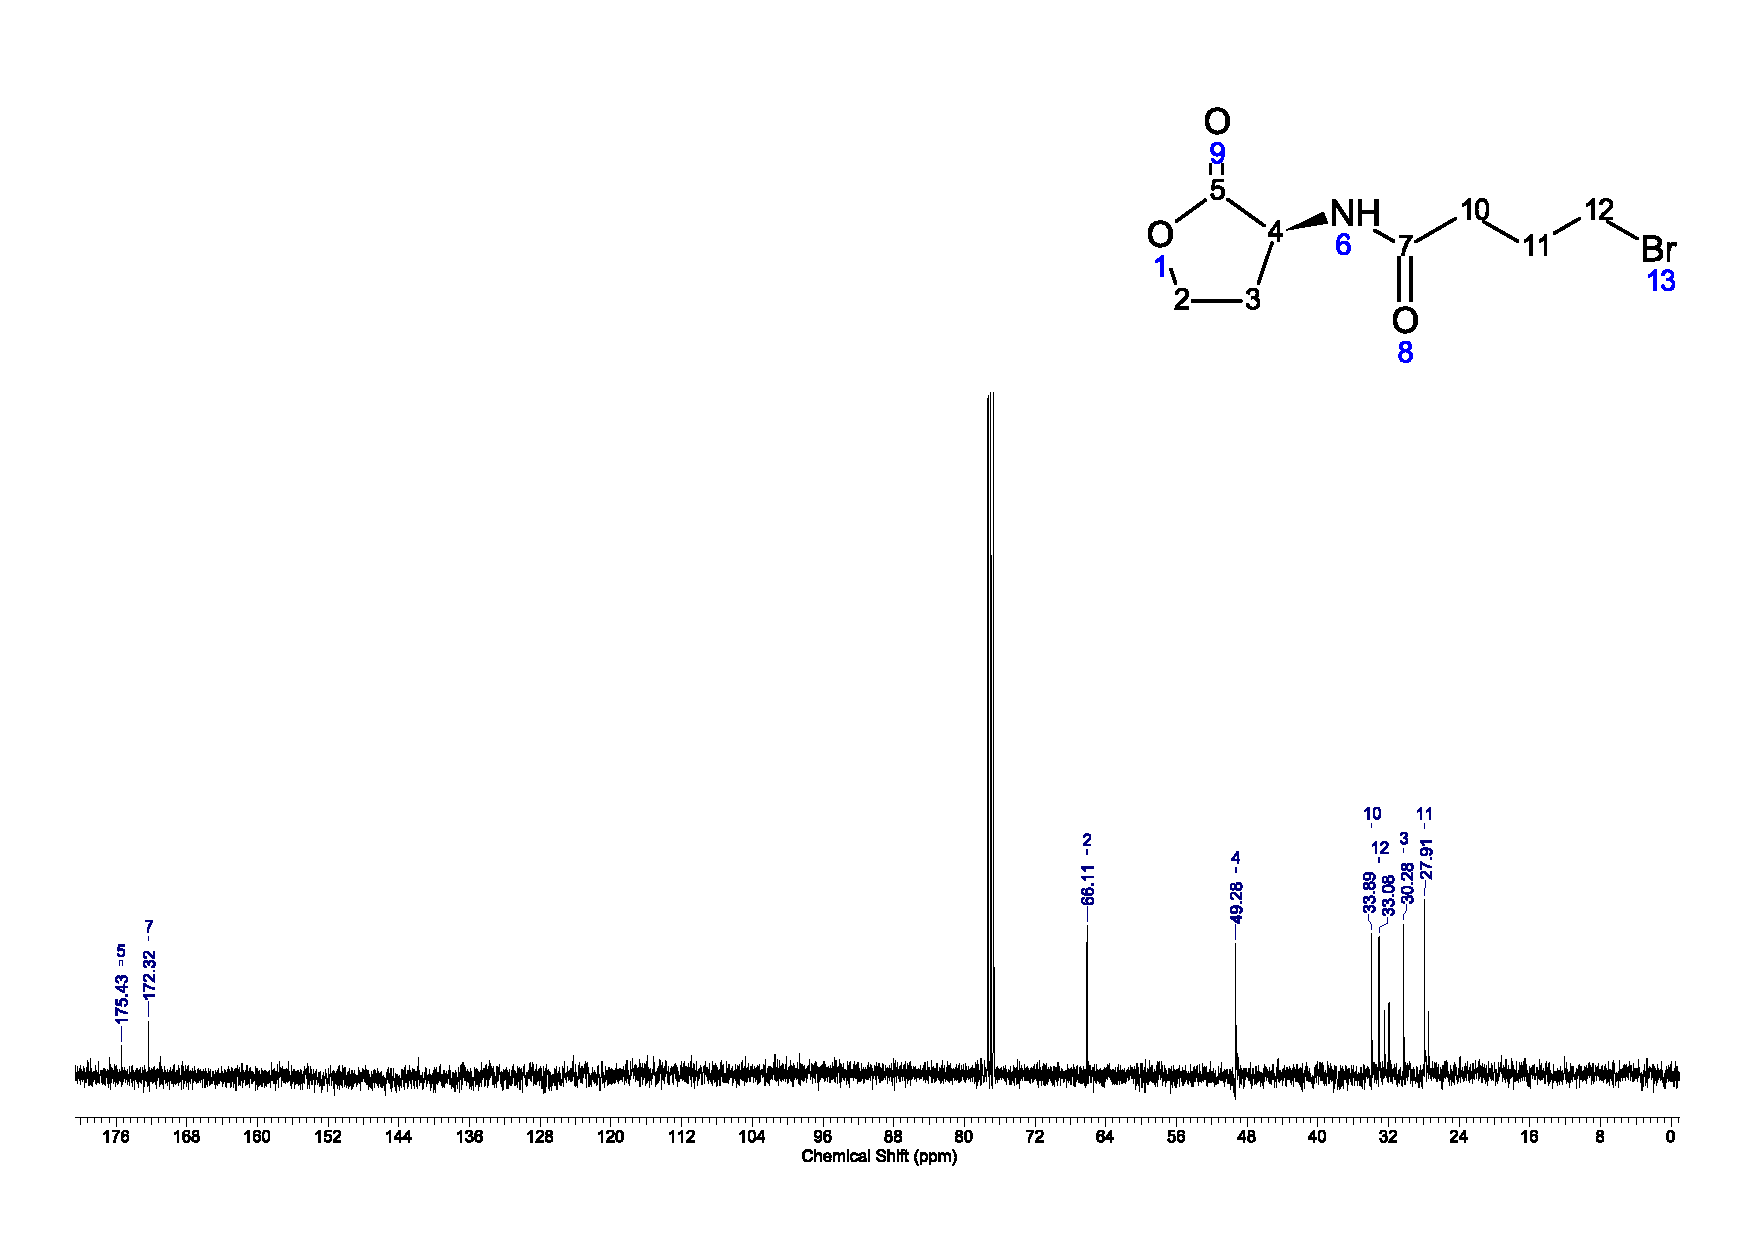
\includegraphics[ width=1.0\textwidth,height=0.43\textheight,keepaspectratio,trim={0 0 0 1.7cm},clip]{HL4Br_C.pdf}
	%\caption{\compound{cmpd:HL4Br}}
\end{figure}

\subsection{(\textit{S})-6-Bromo-\textit{N}-(2-oxotetrahydrofuran-3-yl)hexanamide \compound{cmpd:HL6Br}}

\begin{figure}[H]
	\centering
		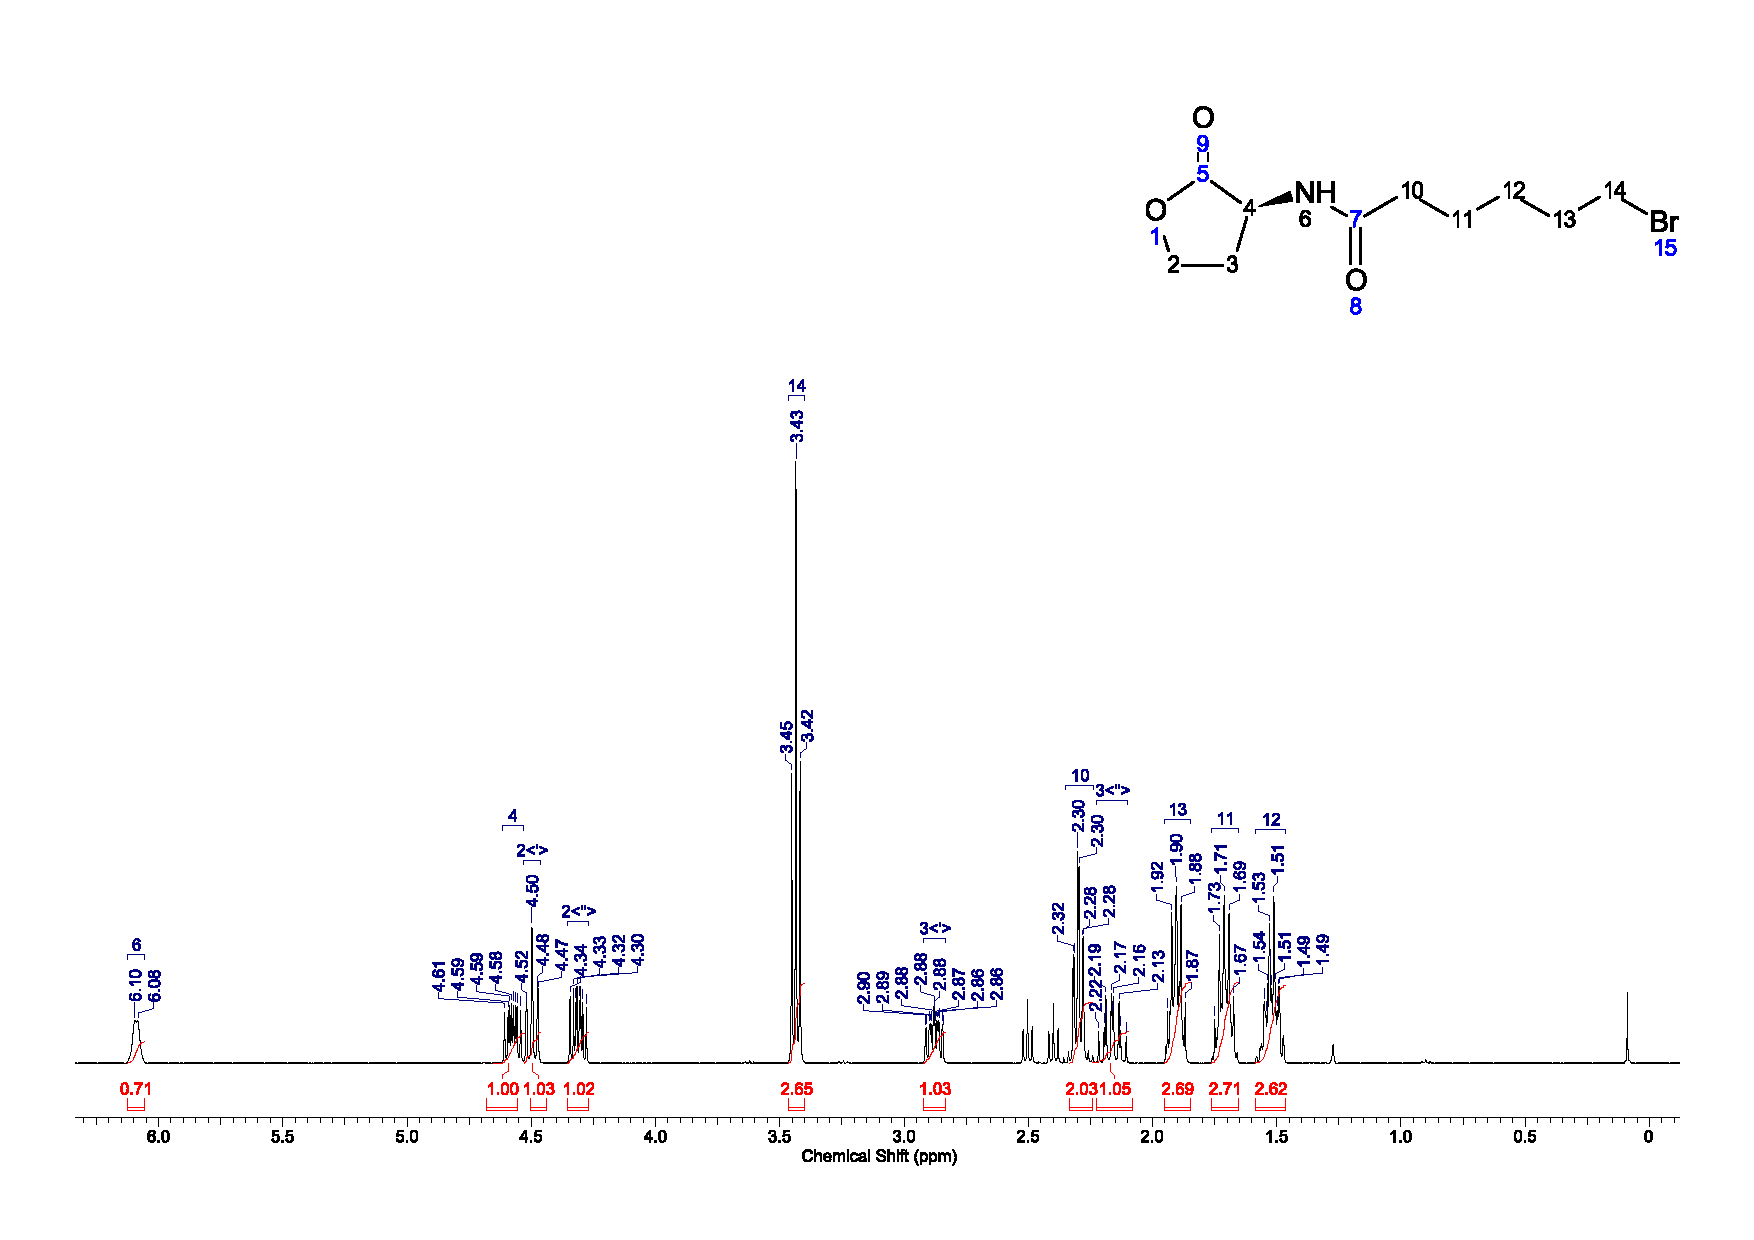
\includegraphics[ width=1.0\textwidth,height=0.43\textheight,keepaspectratio,trim={0 0 0 1.7cm},clip]{HL6Br_H.pdf}
		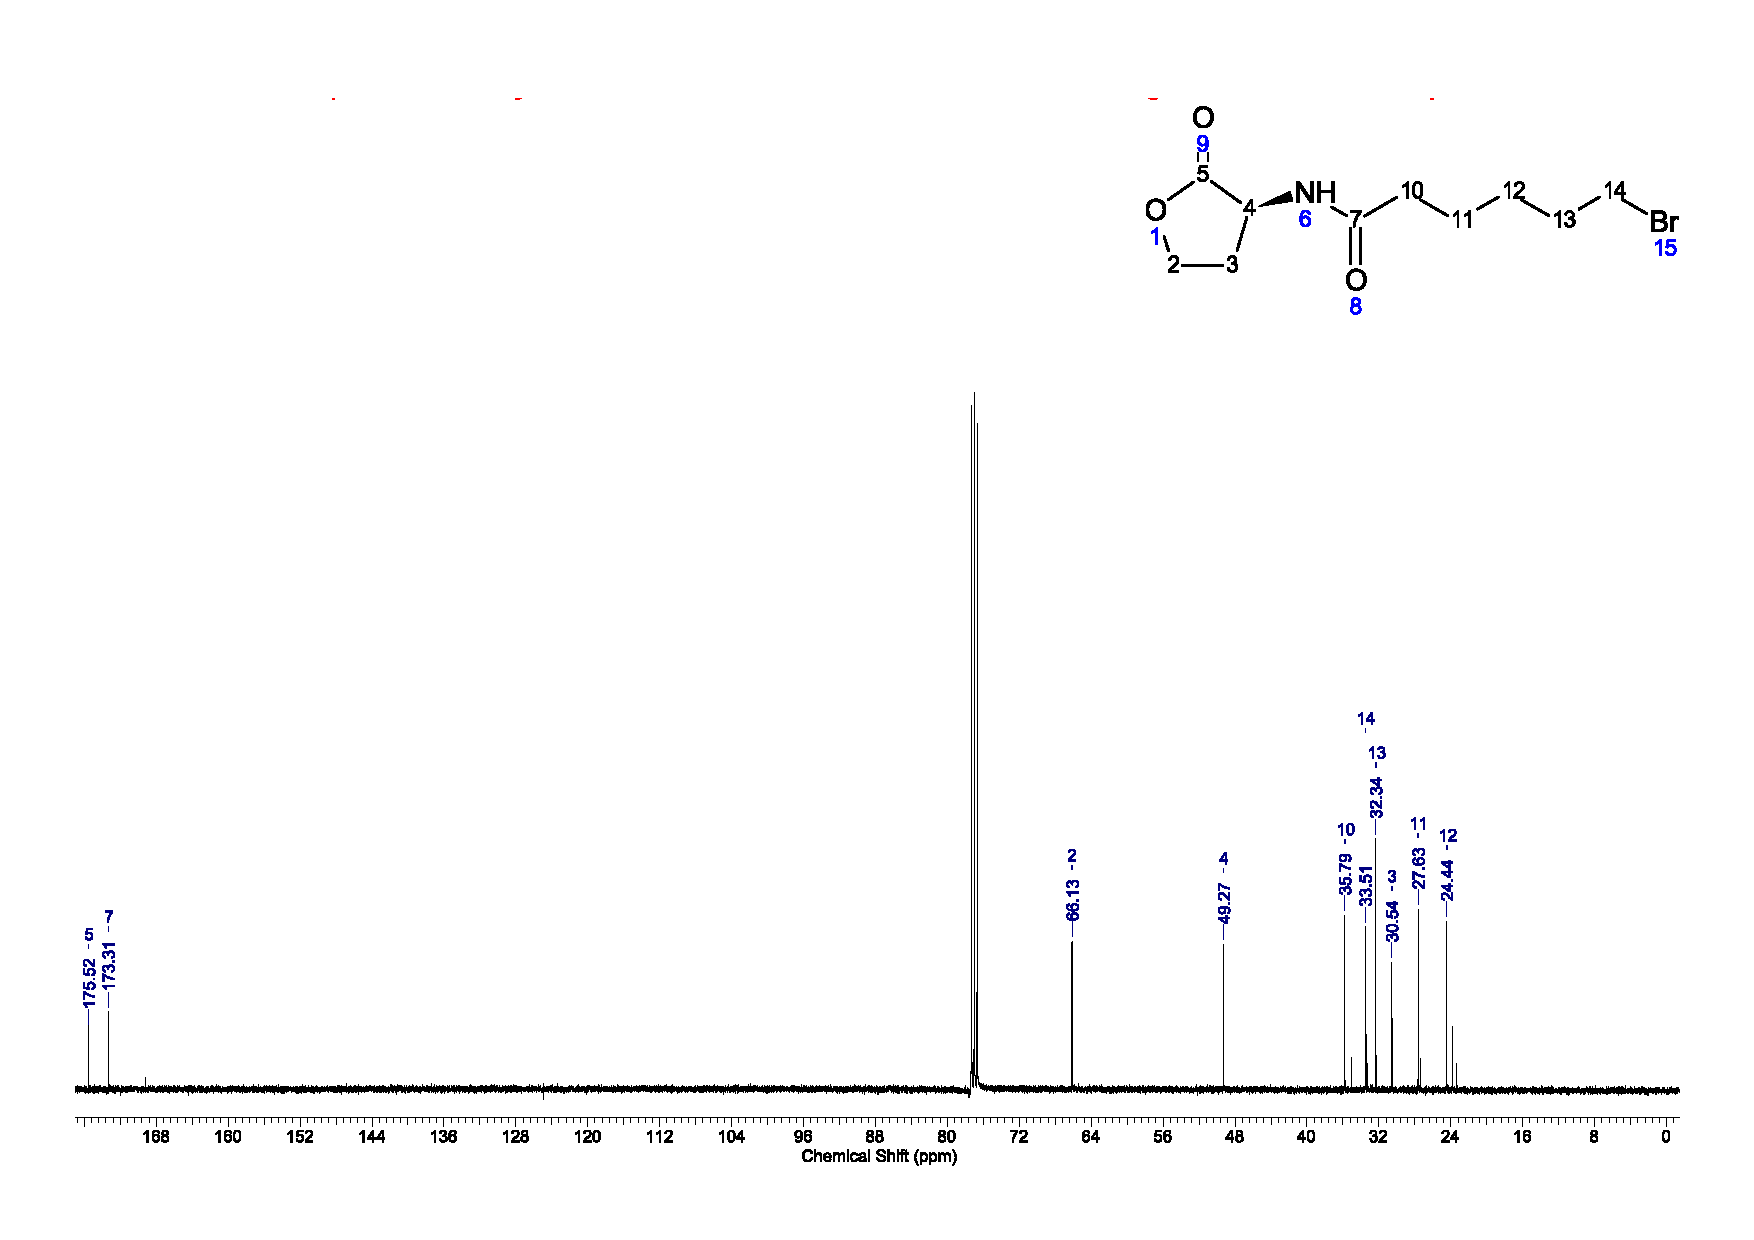
\includegraphics[ width=1.0\textwidth,height=0.43\textheight,keepaspectratio,trim={0 0 0 1.7cm},clip]{HL6Br_C.pdf}
	%\caption{\compound{cmpd:HL6Br}}
\end{figure}

\subsection{(\textit{S})-6-Azido-\textit{N}-(2-oxotetrahydrofuran-3-yl)hexanamide \compound{cmpd:HL6N3}}

\begin{figure}[H]
	\centering
		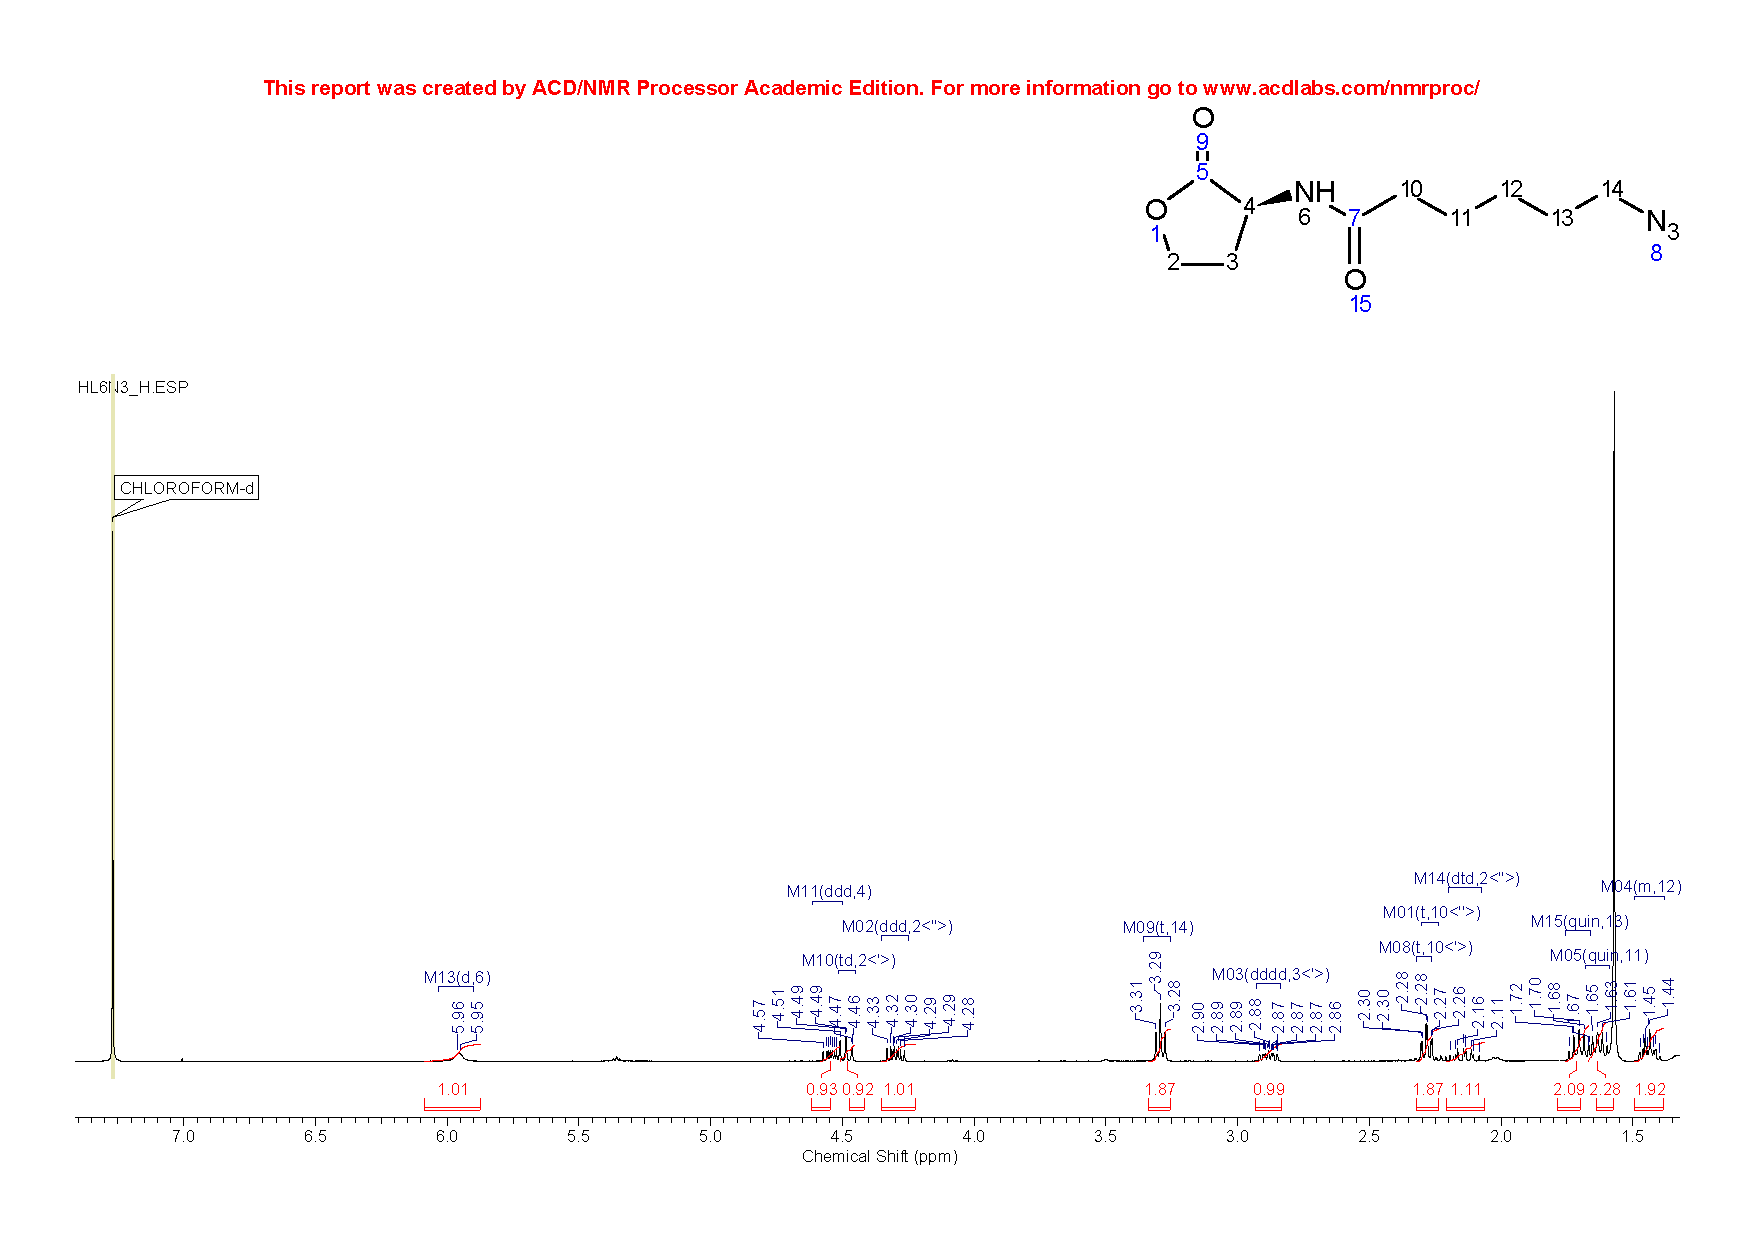
\includegraphics[ width=1.0\textwidth,height=0.43\textheight,keepaspectratio,trim={0 0 0 1.7cm},clip]{HL6N3_H.pdf}
		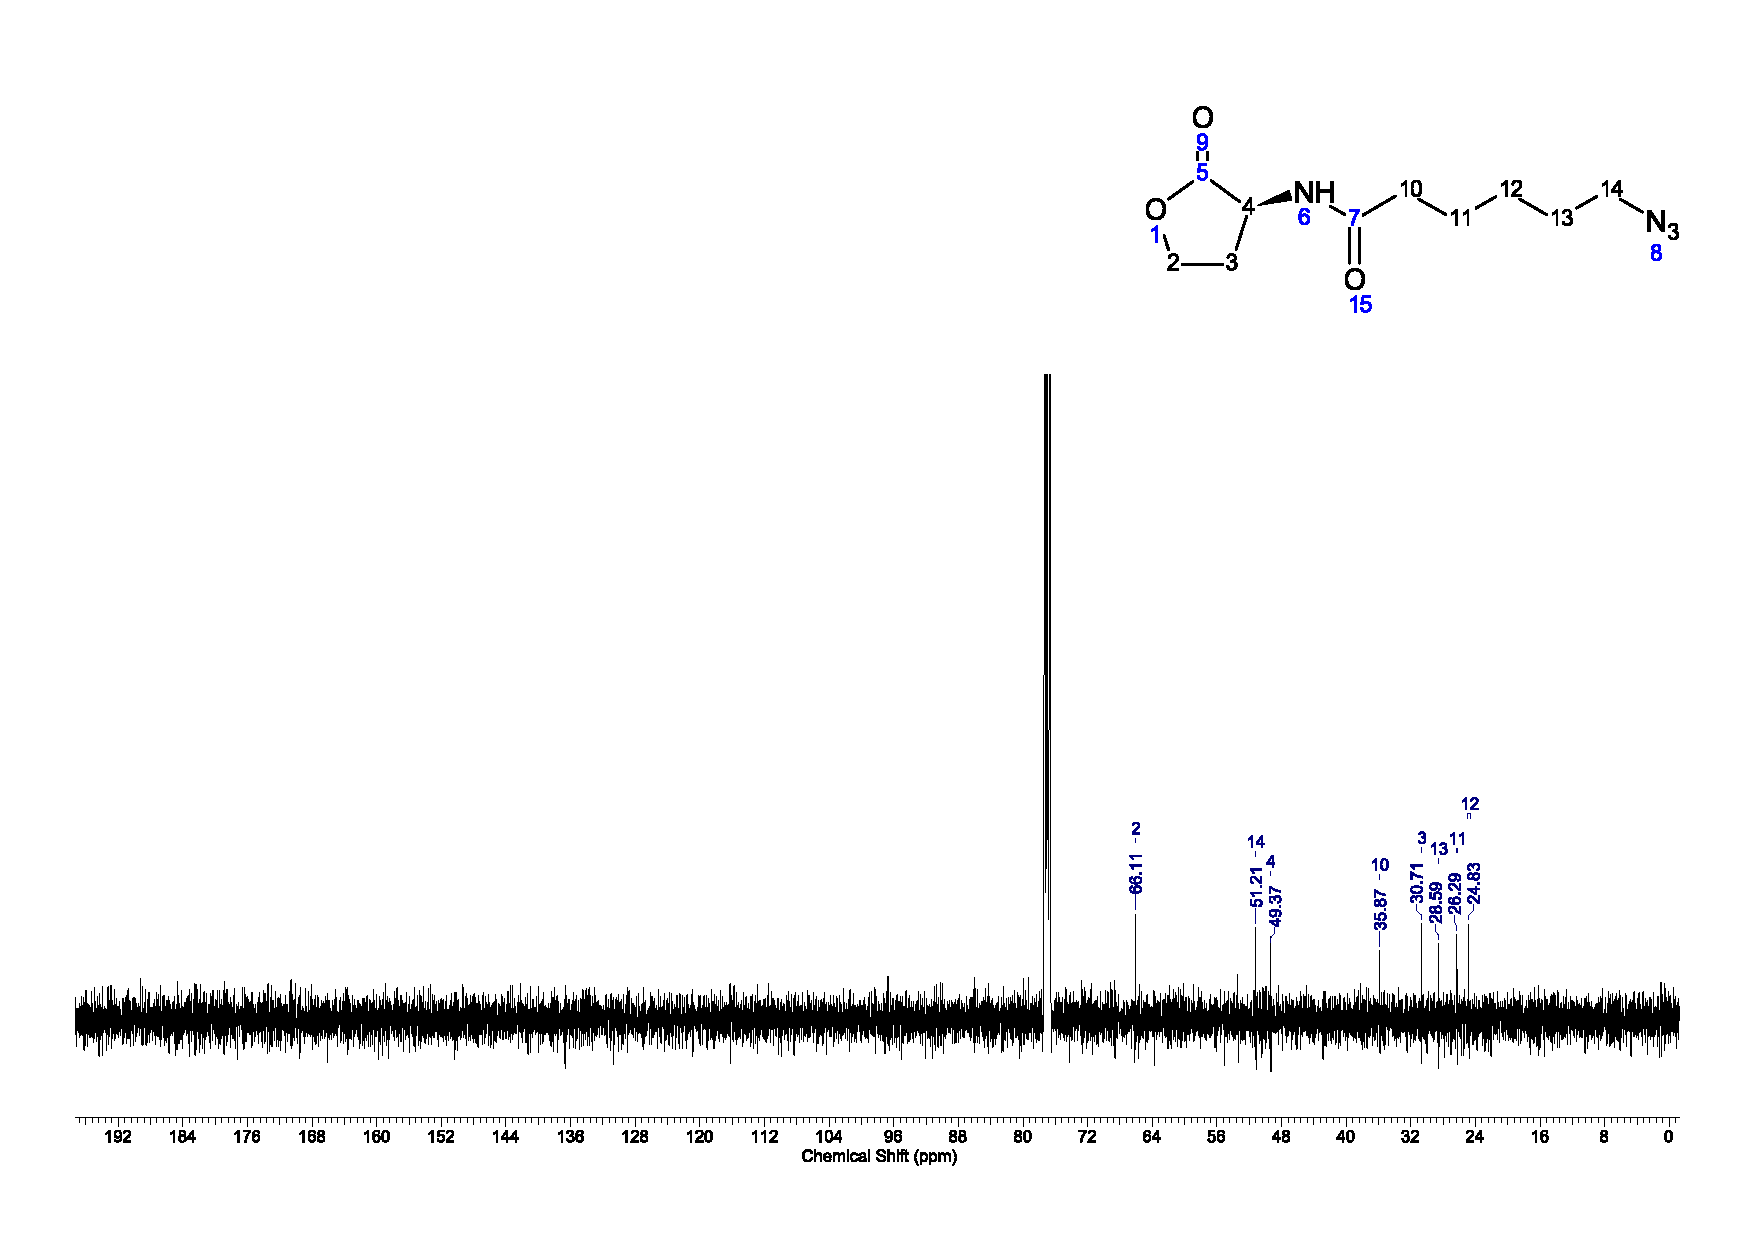
\includegraphics[ width=1.0\textwidth,height=0.43\textheight,keepaspectratio,trim={0 0 0 1.7cm},clip]{HL6N3_C.pdf}
	%\caption{\compound{cmpd:HL6N3}}
\end{figure}

\subsection{\textit{tert}-Butyl 4-(hex-5-yn-1-yl)piperazine-1-carboxylate \compound{cmpd:hexpipboc}}

\begin{figure}[H]
	\centering
		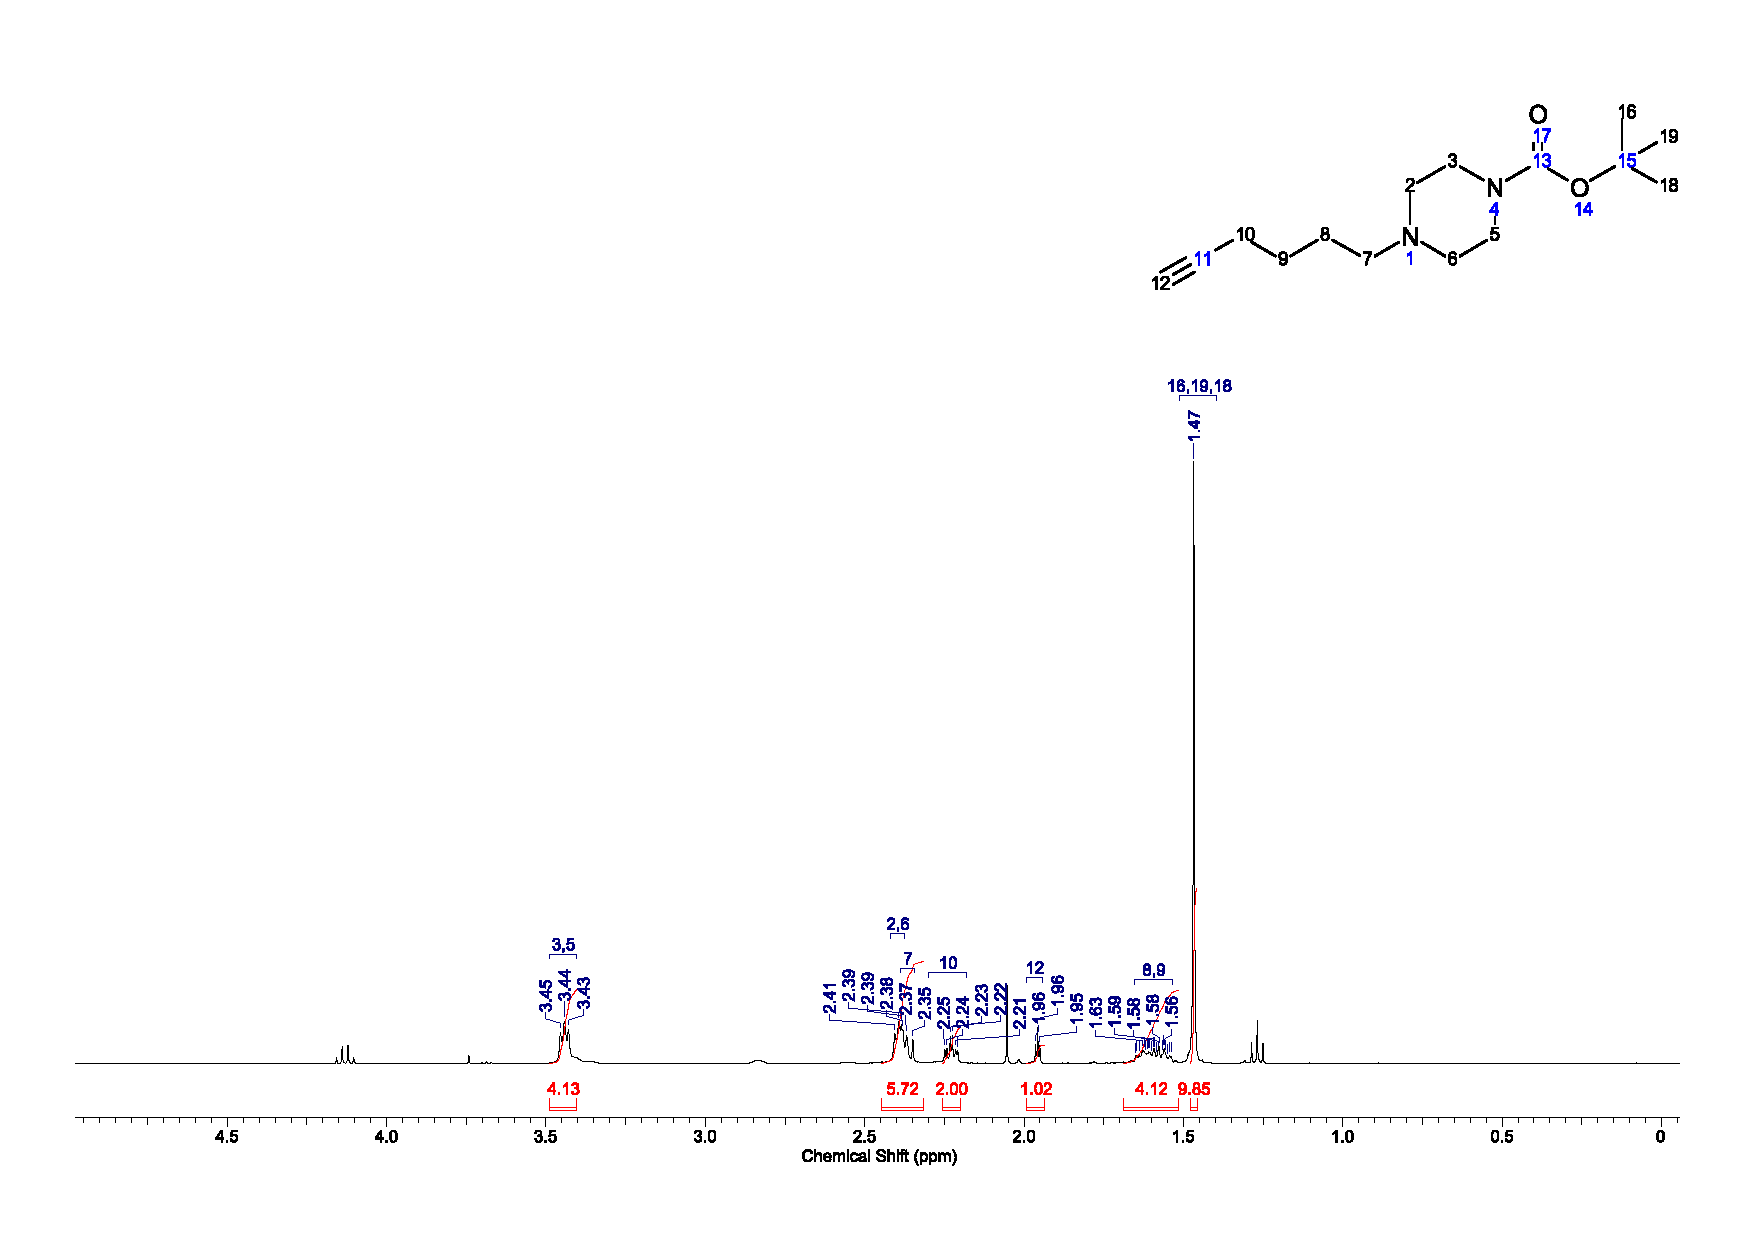
\includegraphics[ width=1.0\textwidth,height=0.43\textheight,keepaspectratio,trim={0 0 0 1.7cm},clip]{hexpipboc_H.pdf}
		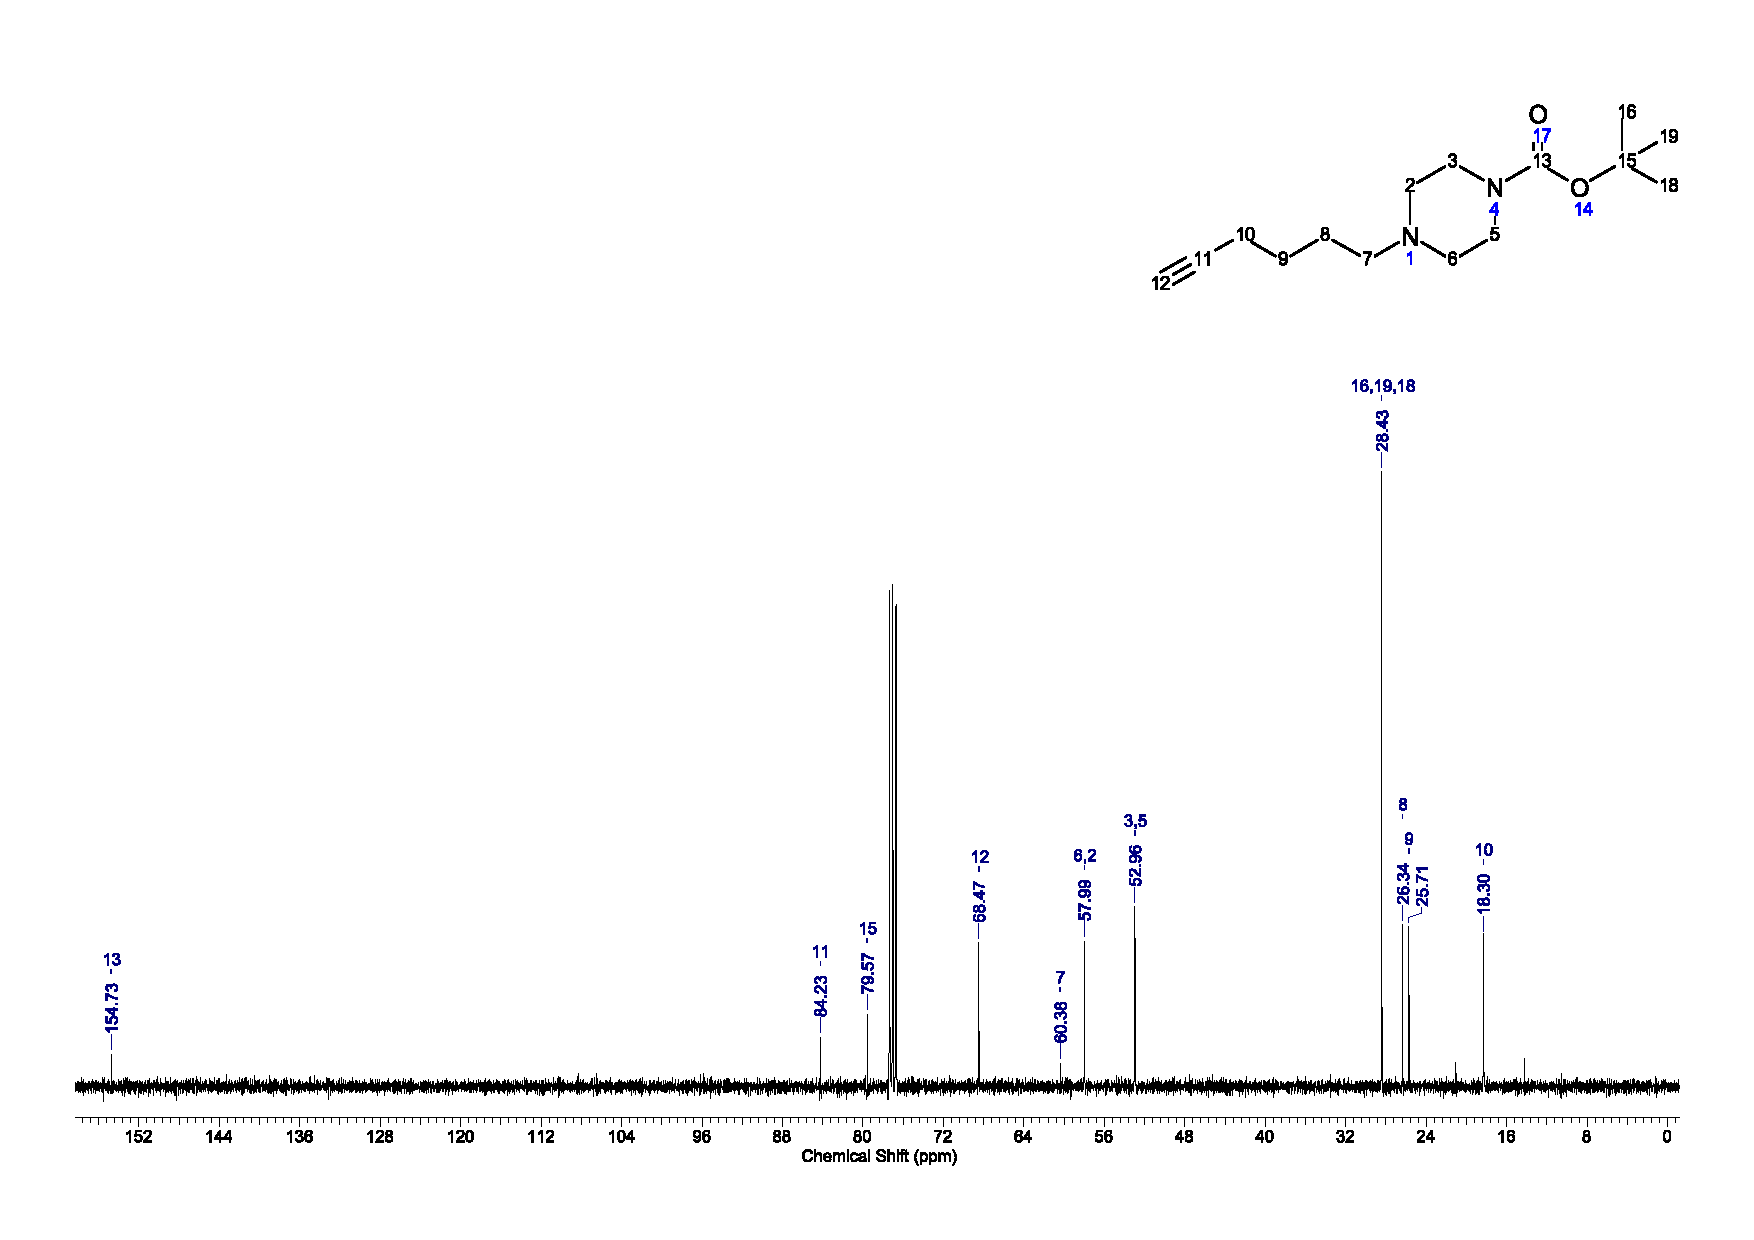
\includegraphics[ width=1.0\textwidth,height=0.43\textheight,keepaspectratio,trim={0 0 0 1.7cm},clip]{hexpipboc_C.pdf}
	%\caption{\compound{cmpd:hexpipboc}}
\end{figure}

\subsection{1-(Hex-5-yn-1-yl)piperazine \compound{cmpd:hexpip}}

\begin{figure}[H]
	\centering
		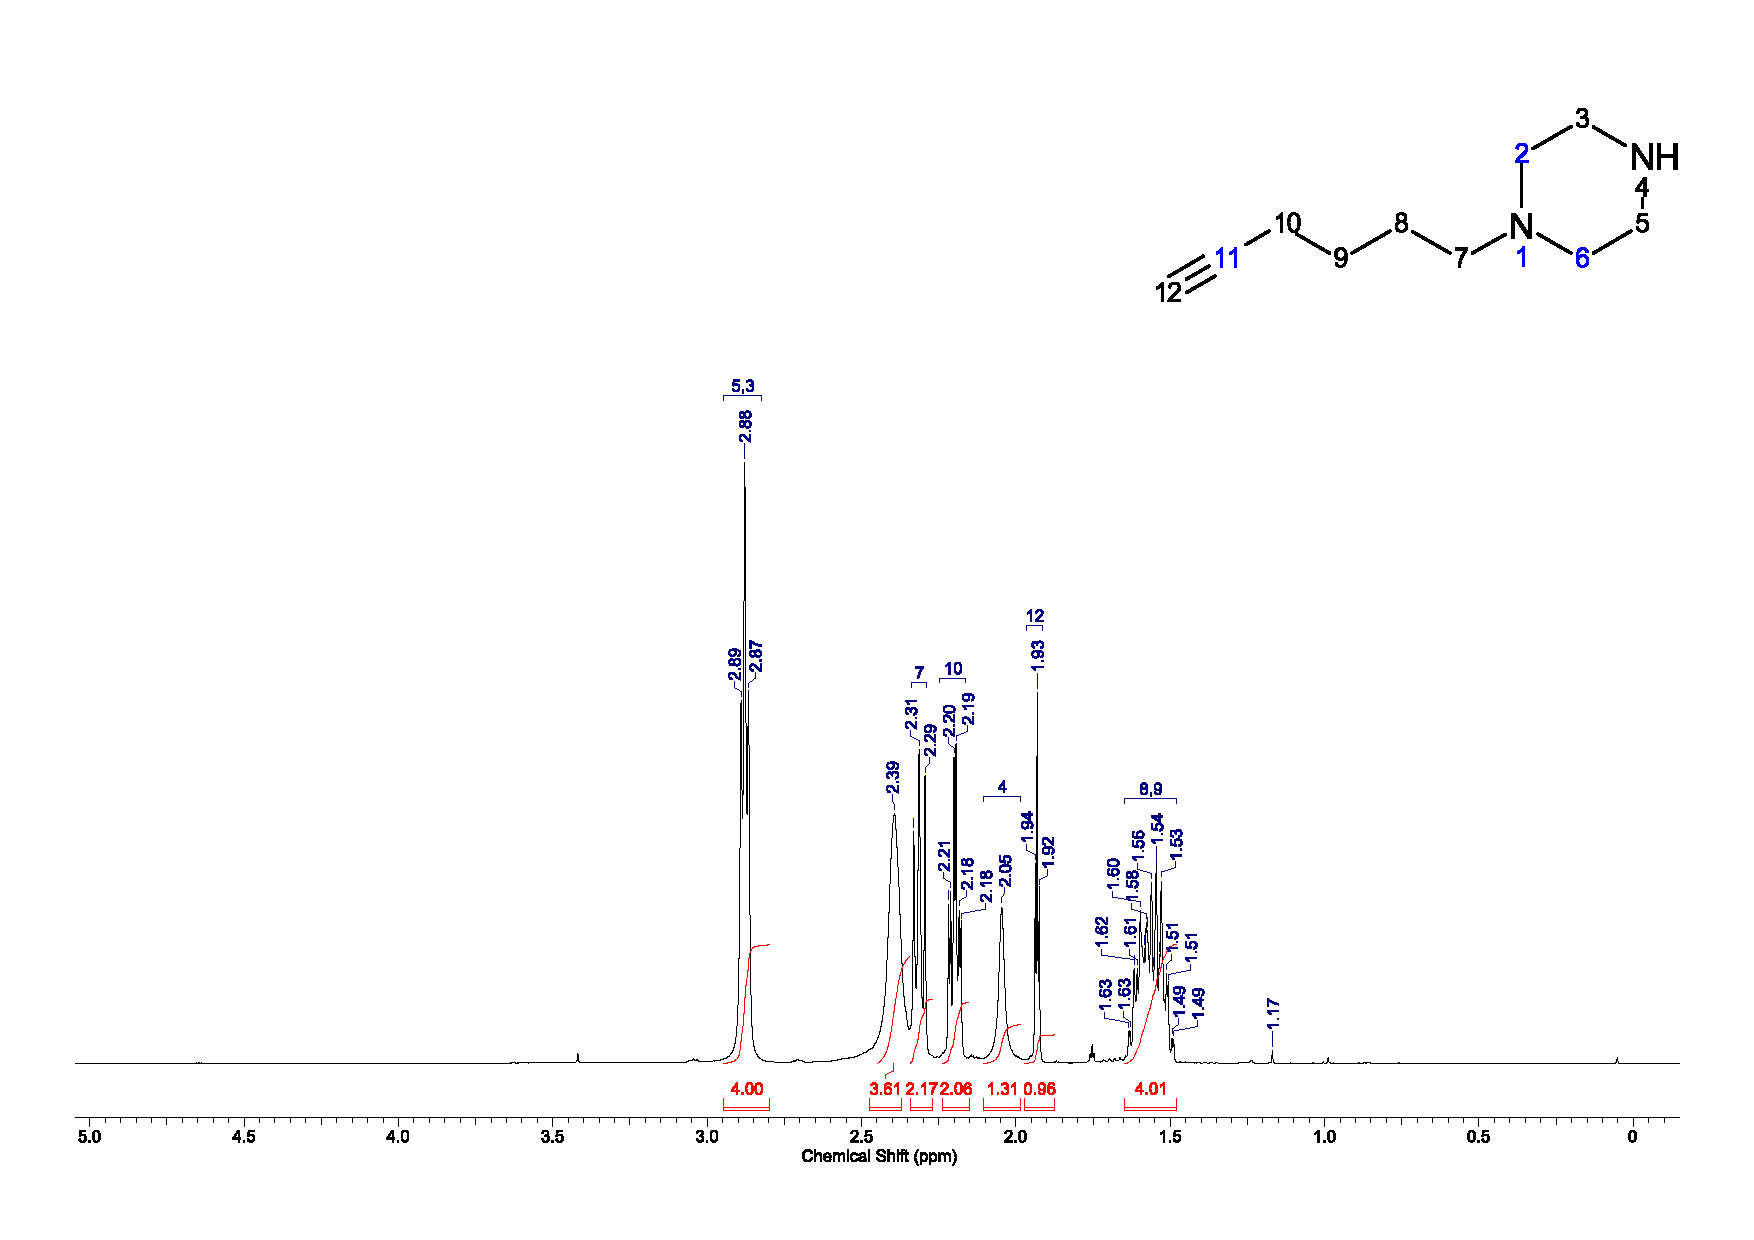
\includegraphics[ width=1.0\textwidth,height=0.43\textheight,keepaspectratio,trim={0 0 0 1.7cm},clip]{hexpip_H.pdf}
		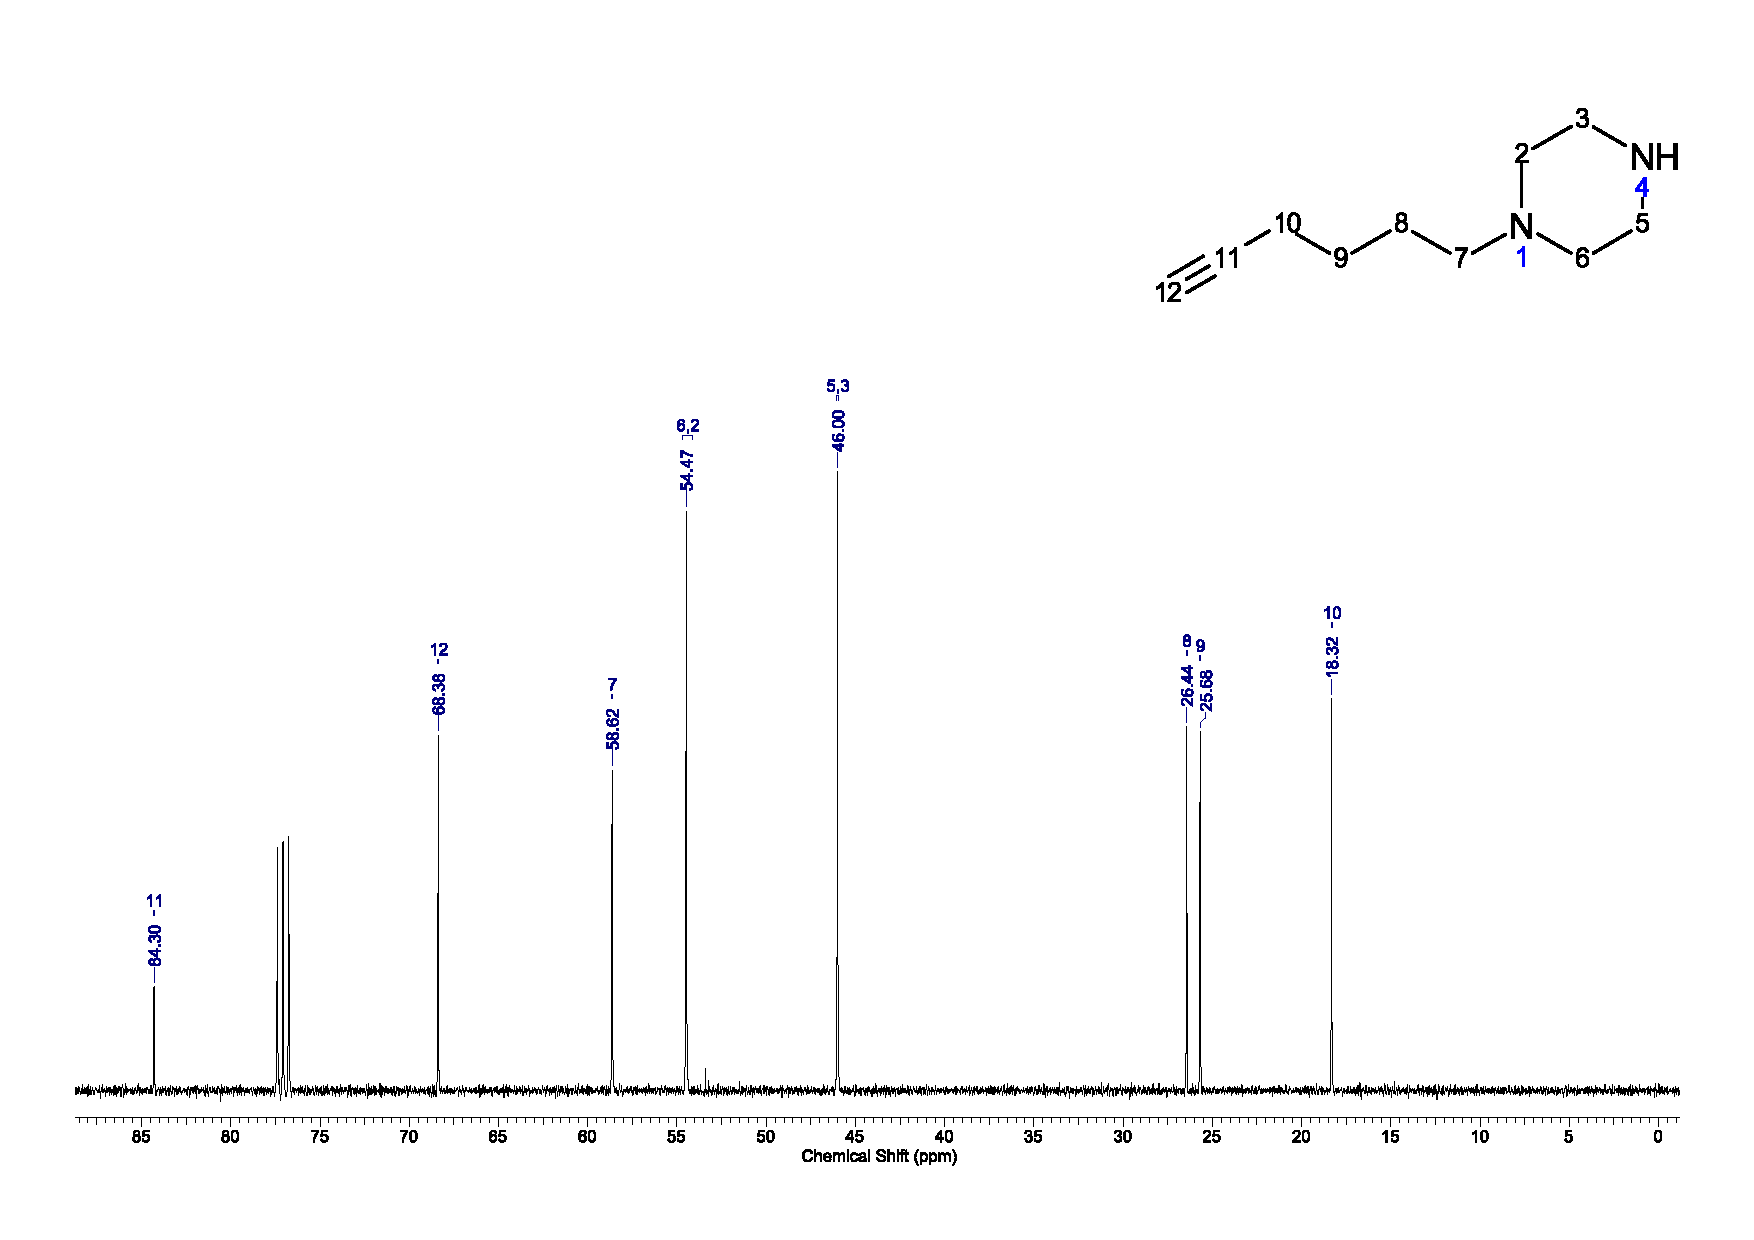
\includegraphics[ width=1.0\textwidth,height=0.43\textheight,keepaspectratio,trim={0 0 0 1.7cm},clip]{hexpip_C.pdf}
	%\caption{\compound{cmpd:hexpip}}
\end{figure}

\subsection{1-Cyclopropyl-6-fluoro-7-(4-(hex-5-yn-1-yl)piperazin-1-yl)-4-oxo-1,4\hyp{}dihydroqu\allowbreak inoline-3-carboxylic acid \compound{cmpd:Y4Cip}}

\begin{figure}[H]
	\centering
		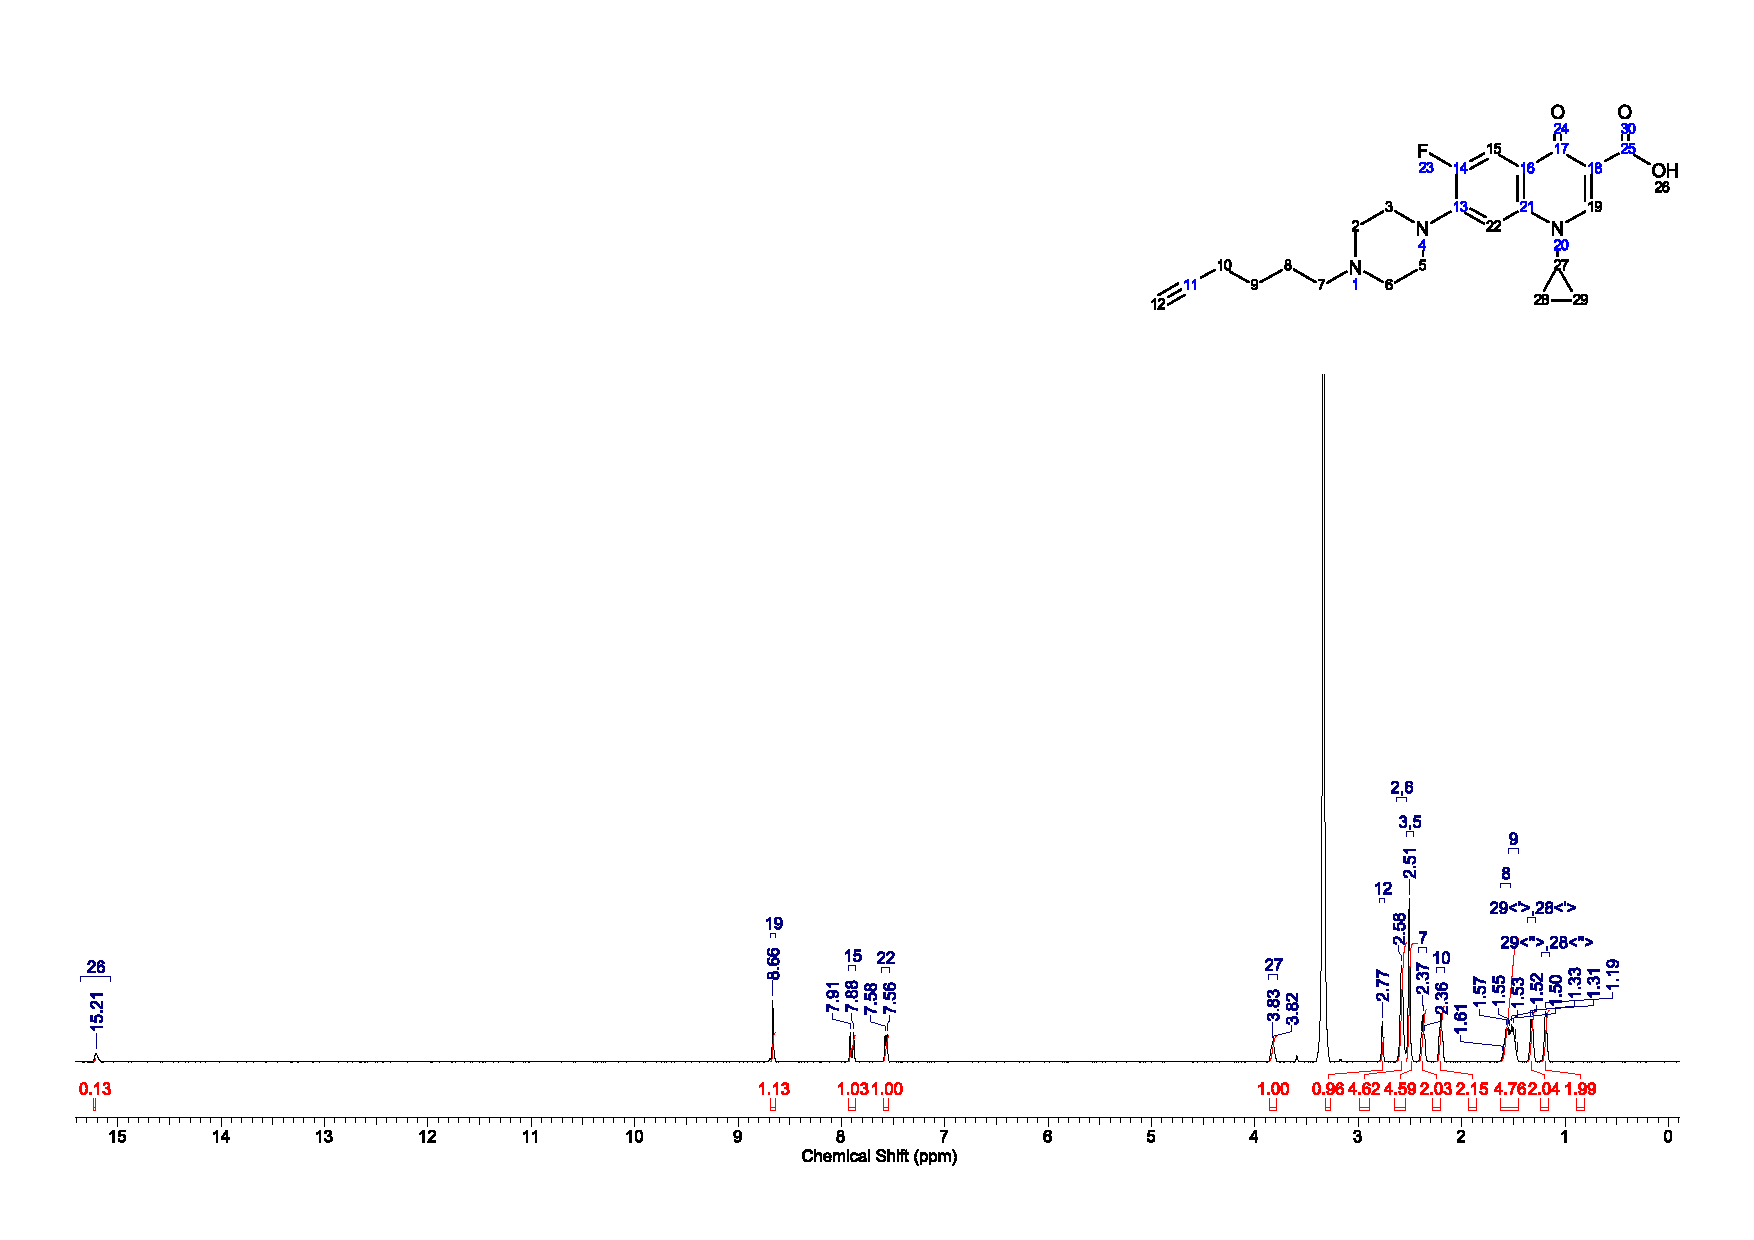
\includegraphics[ width=1.0\textwidth,height=0.43\textheight,keepaspectratio,trim={0 0 0 1.7cm},clip]{hexpipcip_H.pdf}
		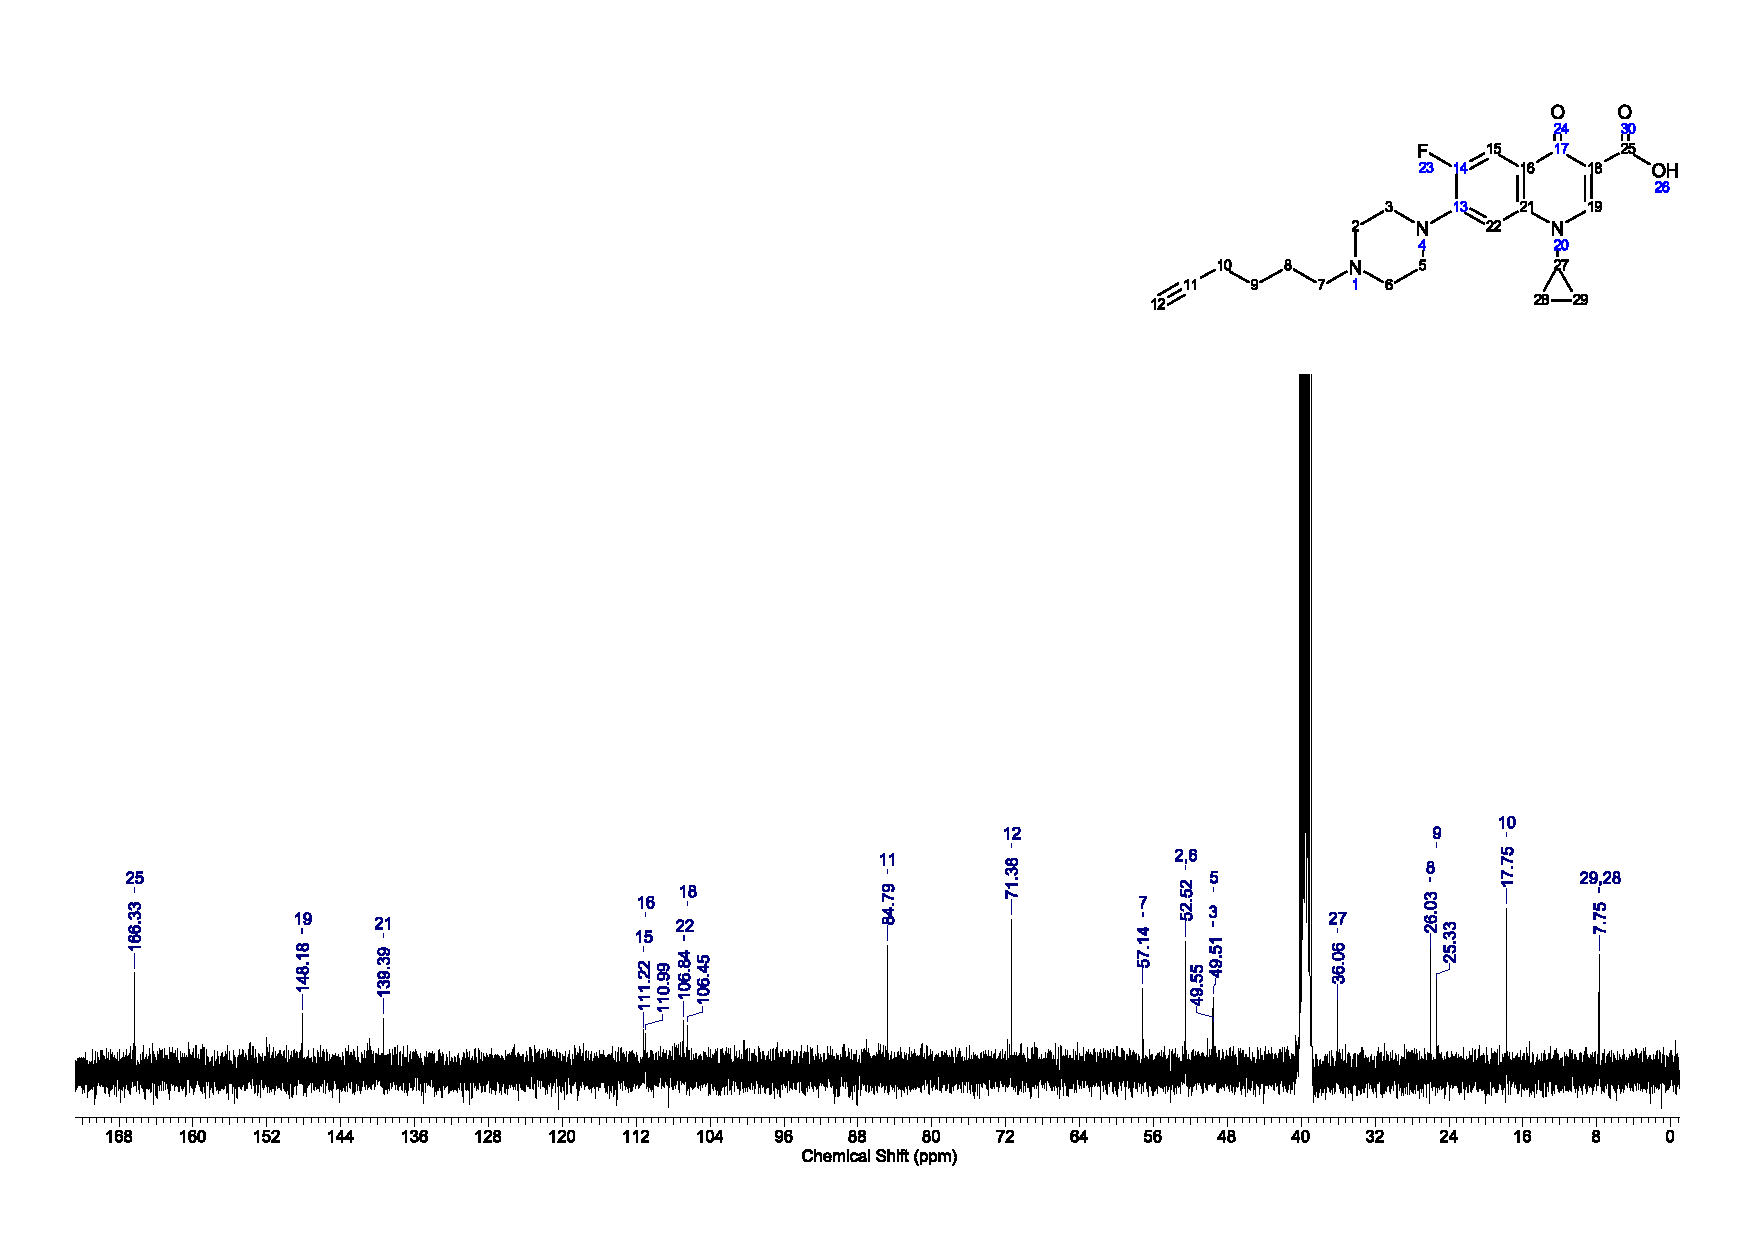
\includegraphics[ width=1.0\textwidth,height=0.43\textheight,keepaspectratio,trim={0 0 0 1.7cm},clip]{hexpipcip_C.pdf}
	%\caption{\compound{cmpd:hexpipcip}}
\end{figure}


%%%%%%%%%%TRIAZOLES%%%%%%%%%%%

\subsection{5-(4-(Hex-5-yn-1-yloxy)-3,5-dimethoxybenzyl)pyrimidine-2,4-diamine \compound{cmpd:Y4Tri}}

\begin{figure}[H]
	\centering
		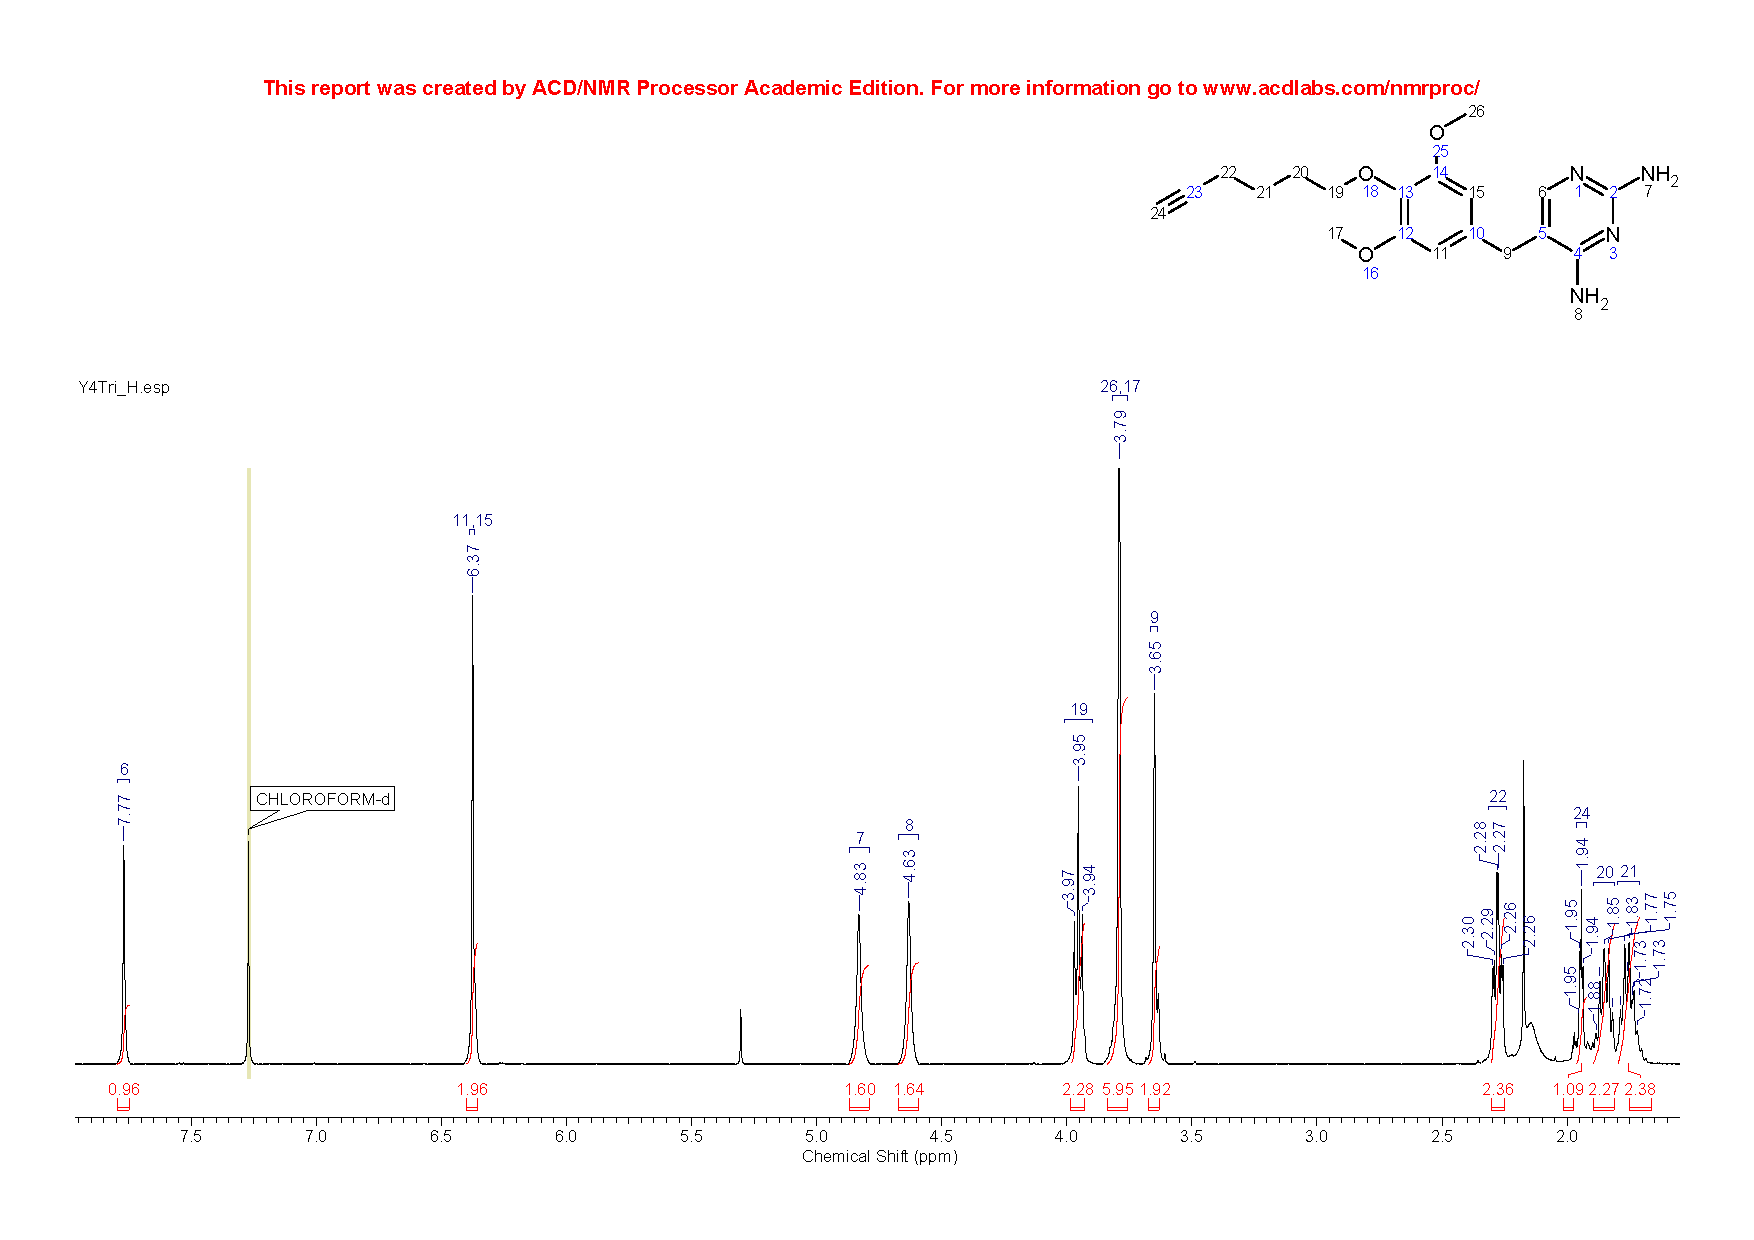
\includegraphics[ width=1.0\textwidth,height=0.43\textheight,keepaspectratio,trim={0 0 0 1.7cm},clip]{Y4Tri_H.pdf}		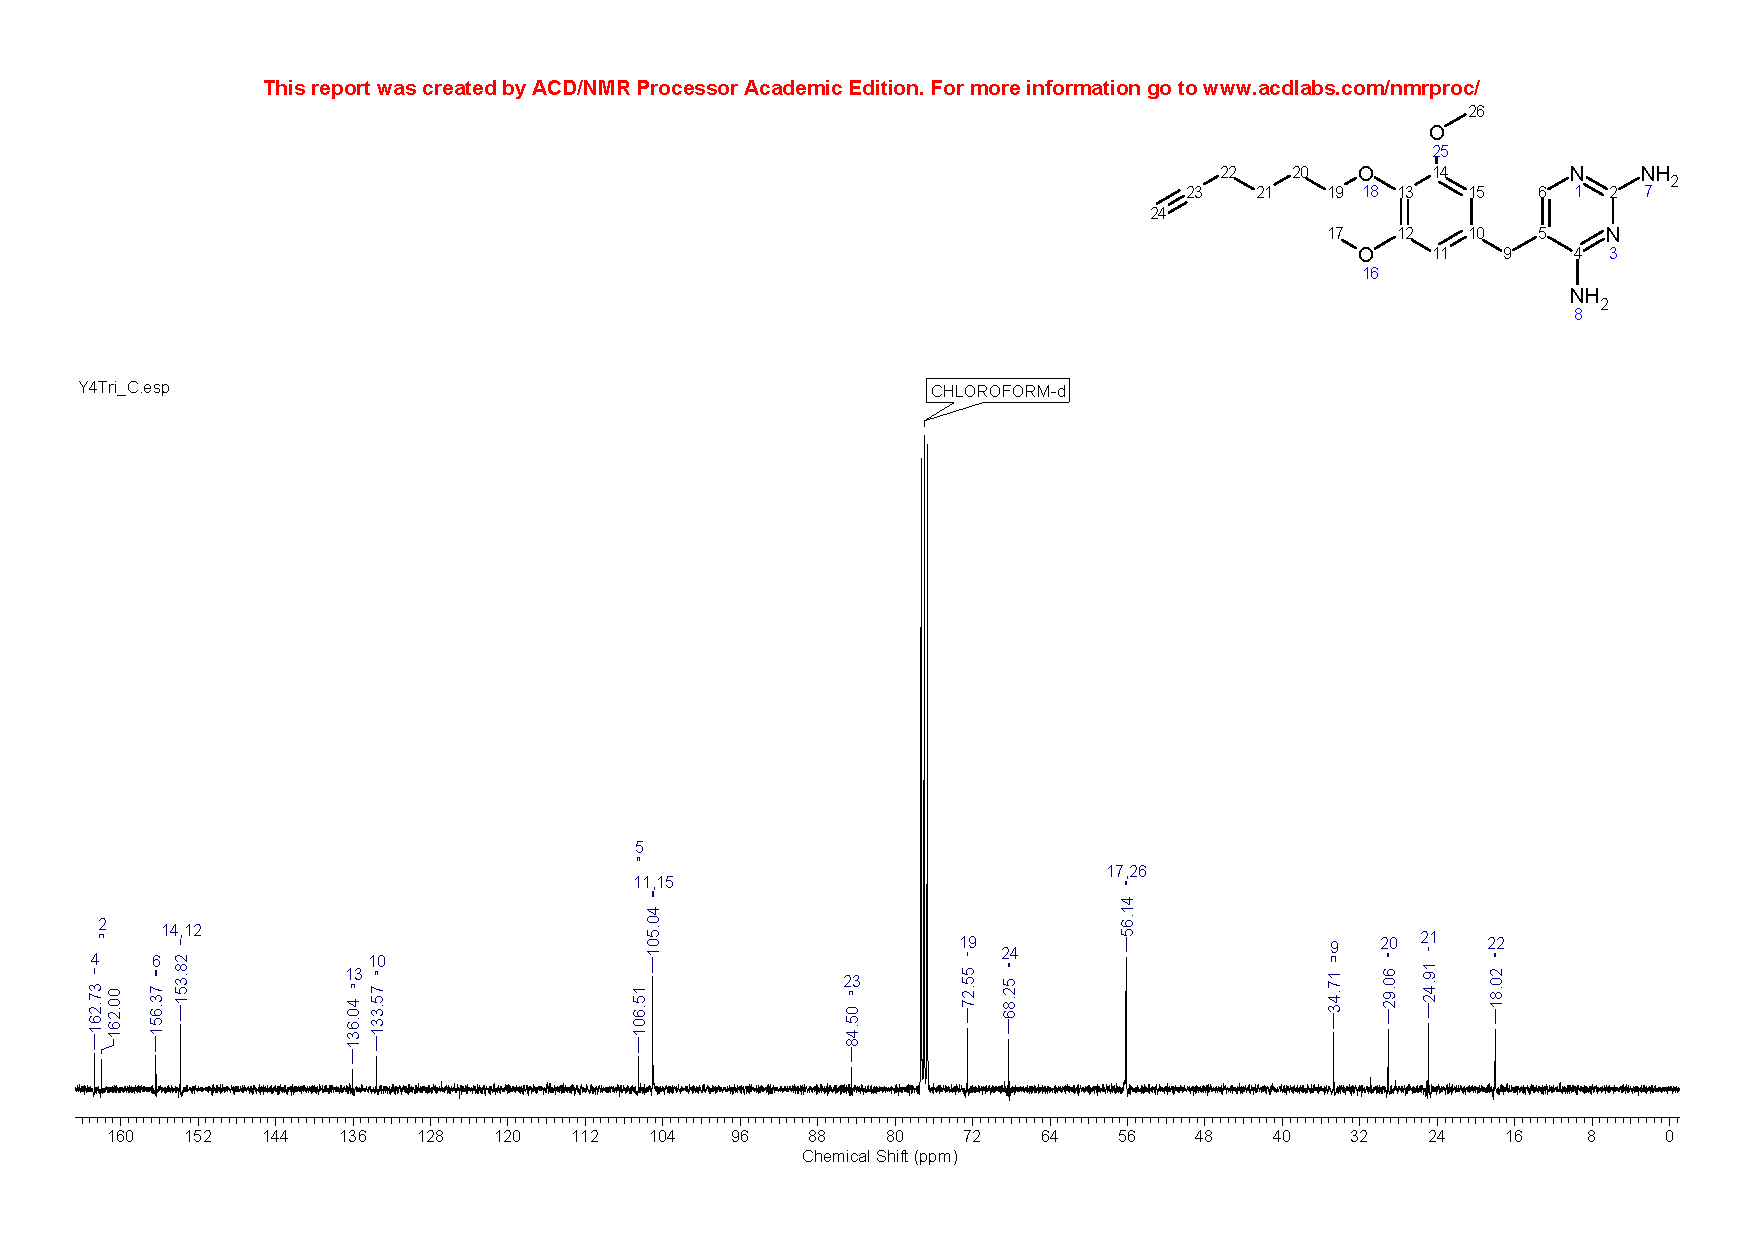
\includegraphics[ width=1.0\textwidth,height=0.43\textheight,keepaspectratio,trim={0 0 0 1.7cm},clip]{Y4Tri_C.pdf}
\end{figure}

\subsection{(\textit{S})-1-Cyclopropyl-6-fluoro-4-oxo-7-(4-(4-(1-(2-oxo-2-((2-oxotetrahydrofuran-3\allowbreak -yl)amino)ethyl)-1\textit{H}-1,2,3-triazol-4-yl)butyl)piperazin-1-yl)-1,4-dihydroquinol\allowbreak ine-3-carboxylic acid \compound{cmpd:HL2T4Cip}}

\begin{figure}[H]
	\centering
		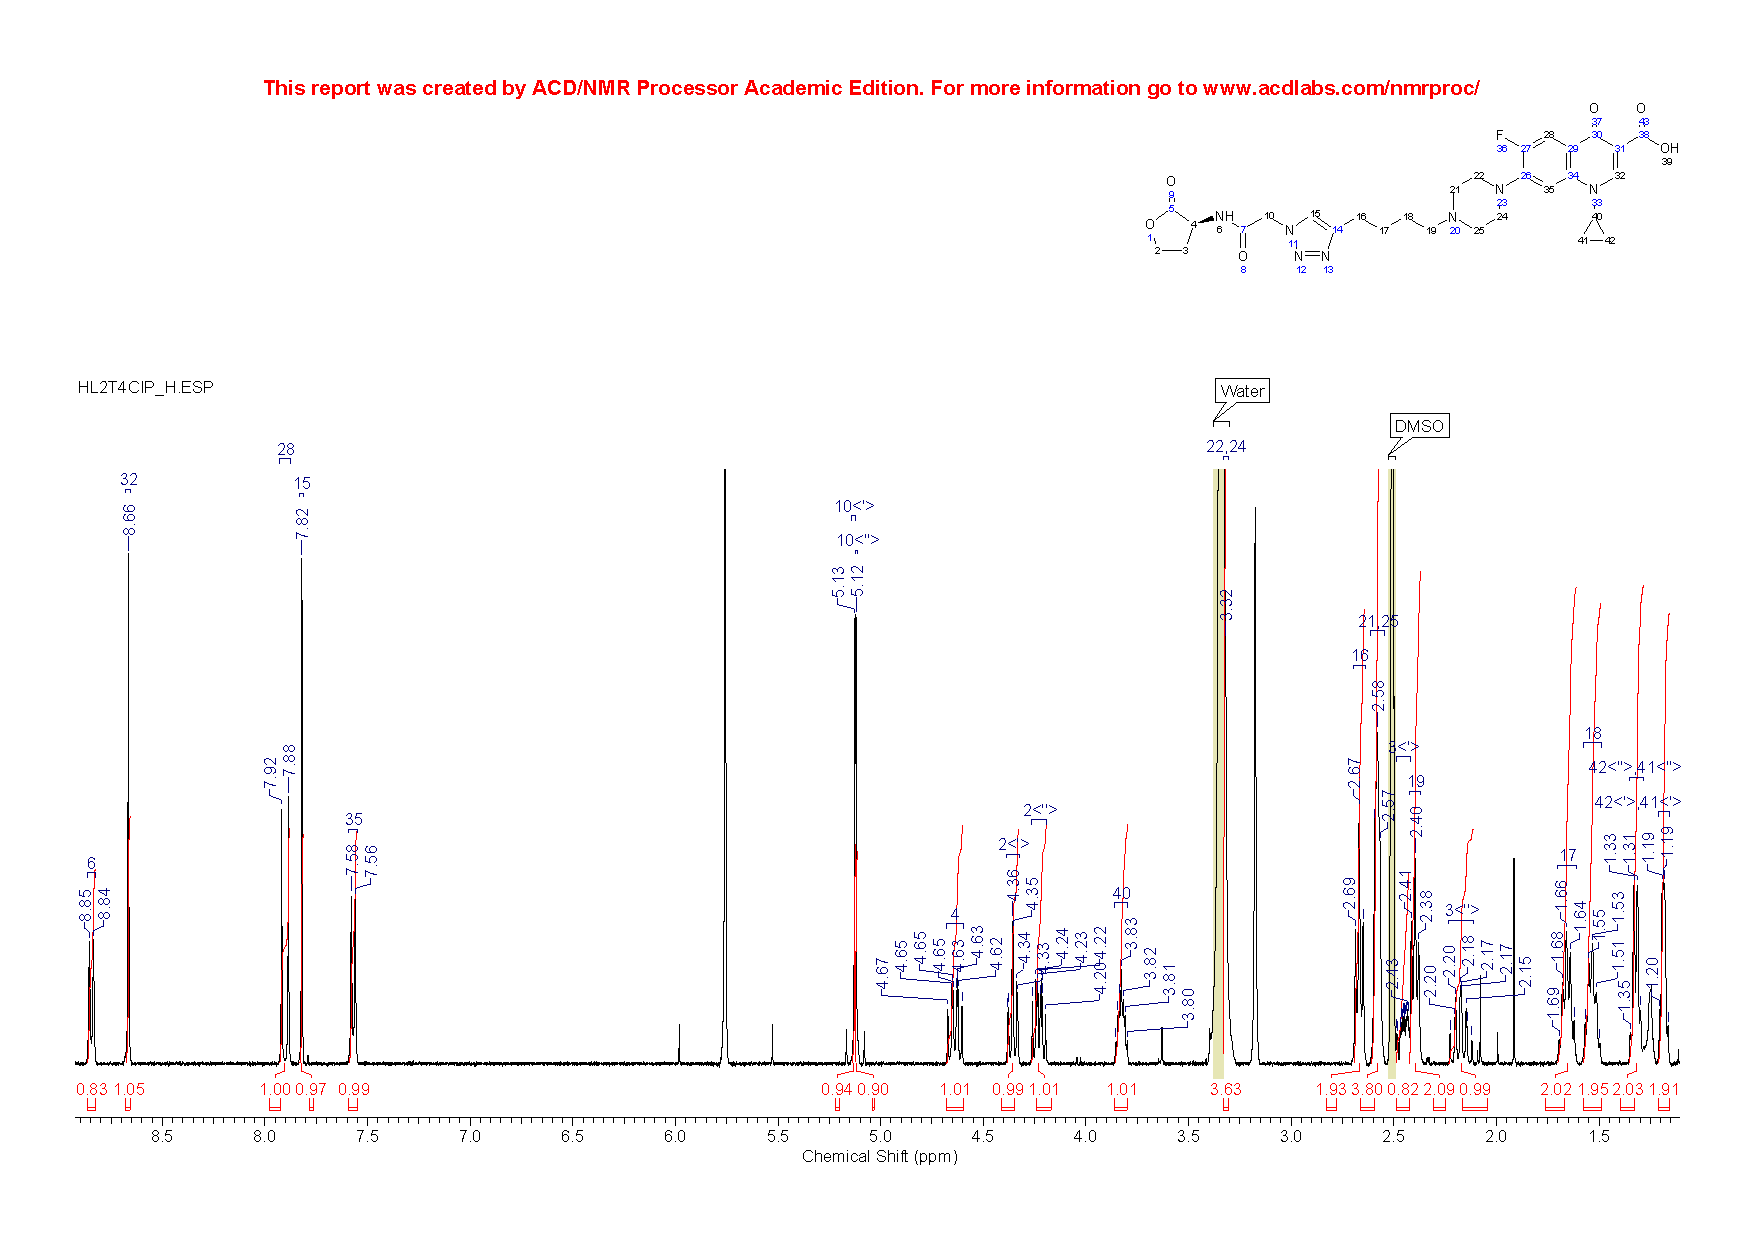
\includegraphics[ width=1.0\textwidth,height=0.43\textheight,keepaspectratio,trim={0 0 0 1.7cm},clip]{HL2T4Cip_H.pdf}
		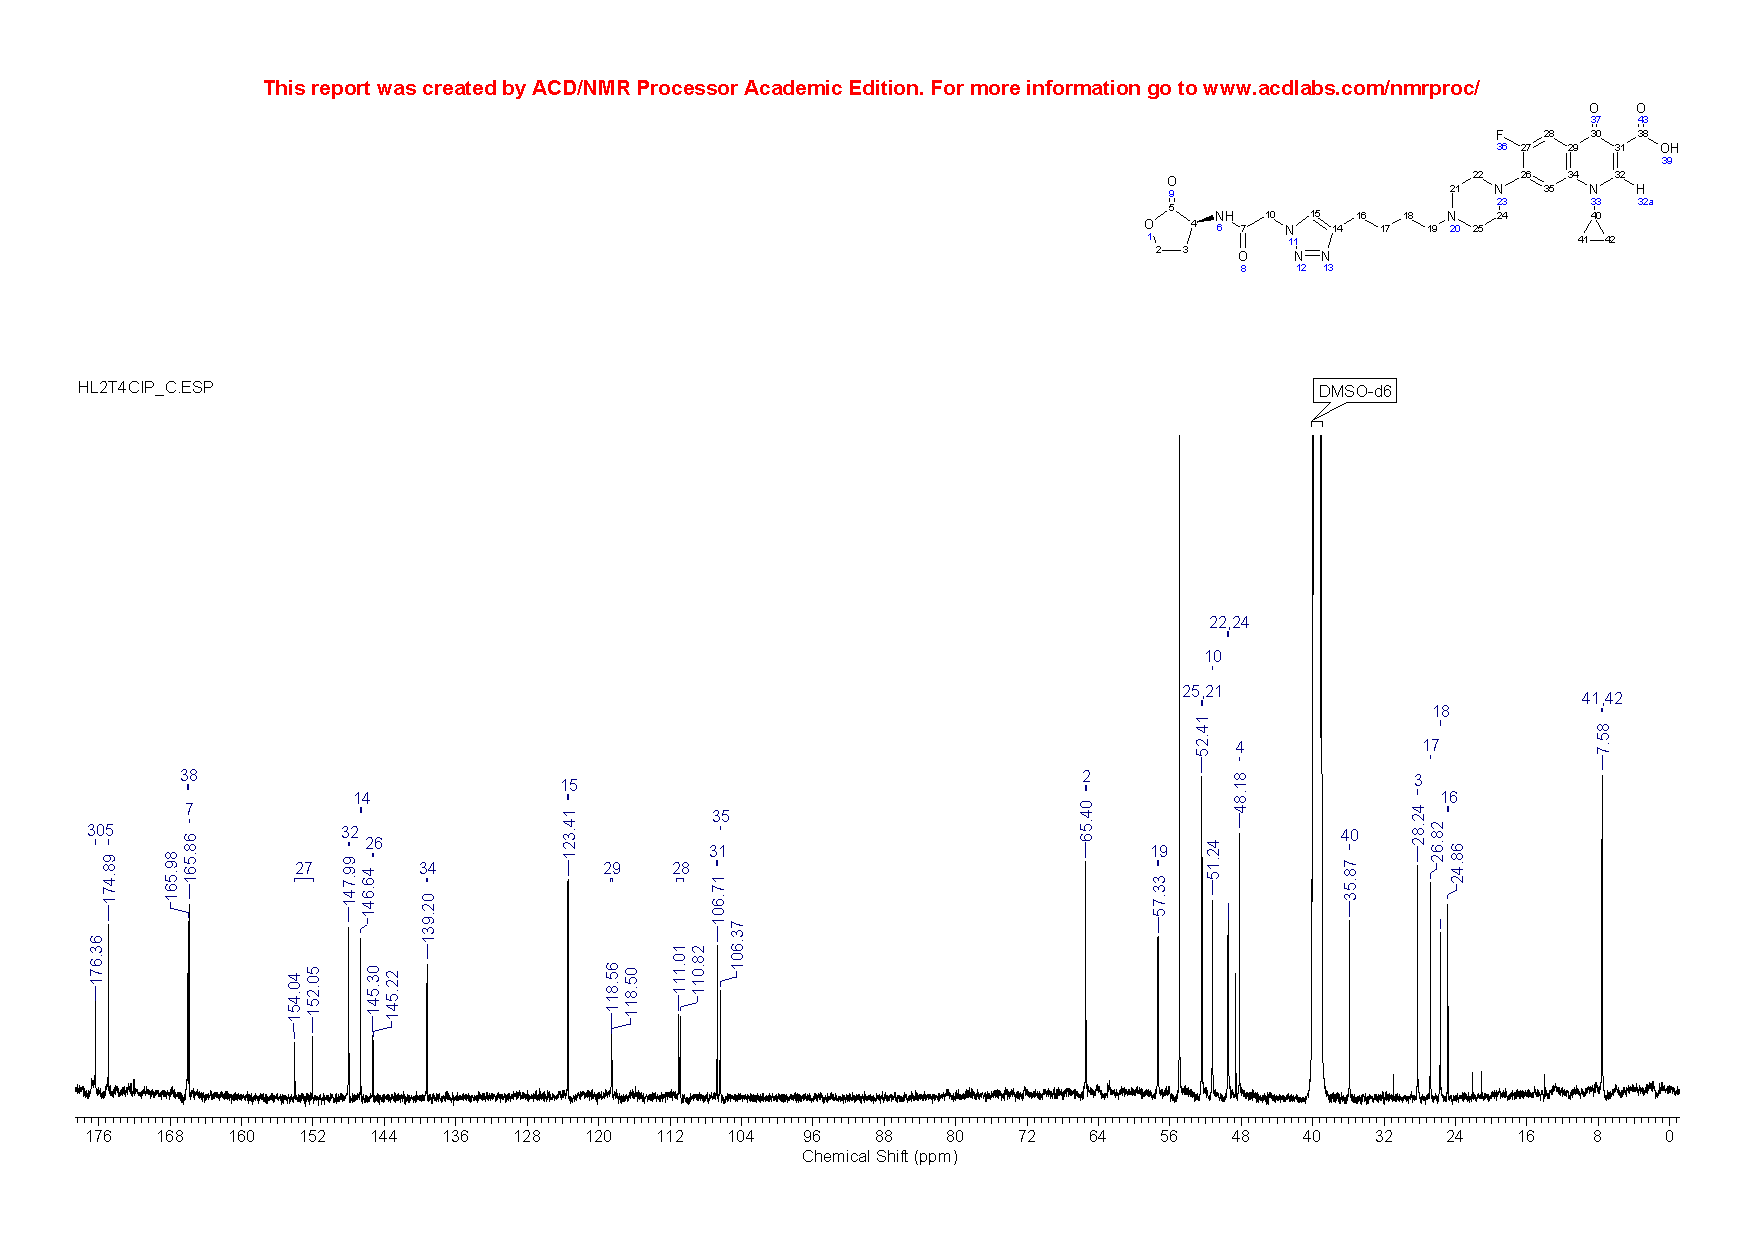
\includegraphics[ width=1.0\textwidth,height=0.43\textheight,keepaspectratio,trim={0 0 0 1.7cm},clip]{HL2T4Cip_C.pdf}
\end{figure}

\subsection{(\textit{S})-1-Cyclopropyl-6-fluoro-4-oxo-7-(4-(4-(1-(4-oxo-4-((2-oxotetrahydrofuran-3\allowbreak -yl)amino)butyl)-1\textit{H}-1,2,3-triazol-4-yl)butyl)piperazin-1-yl)-1,4-dihydroquinol\allowbreak ine-3-carboxylic acid \compound{cmpd:HL4T4Cip}}

\begin{figure}[H]
	\centering
		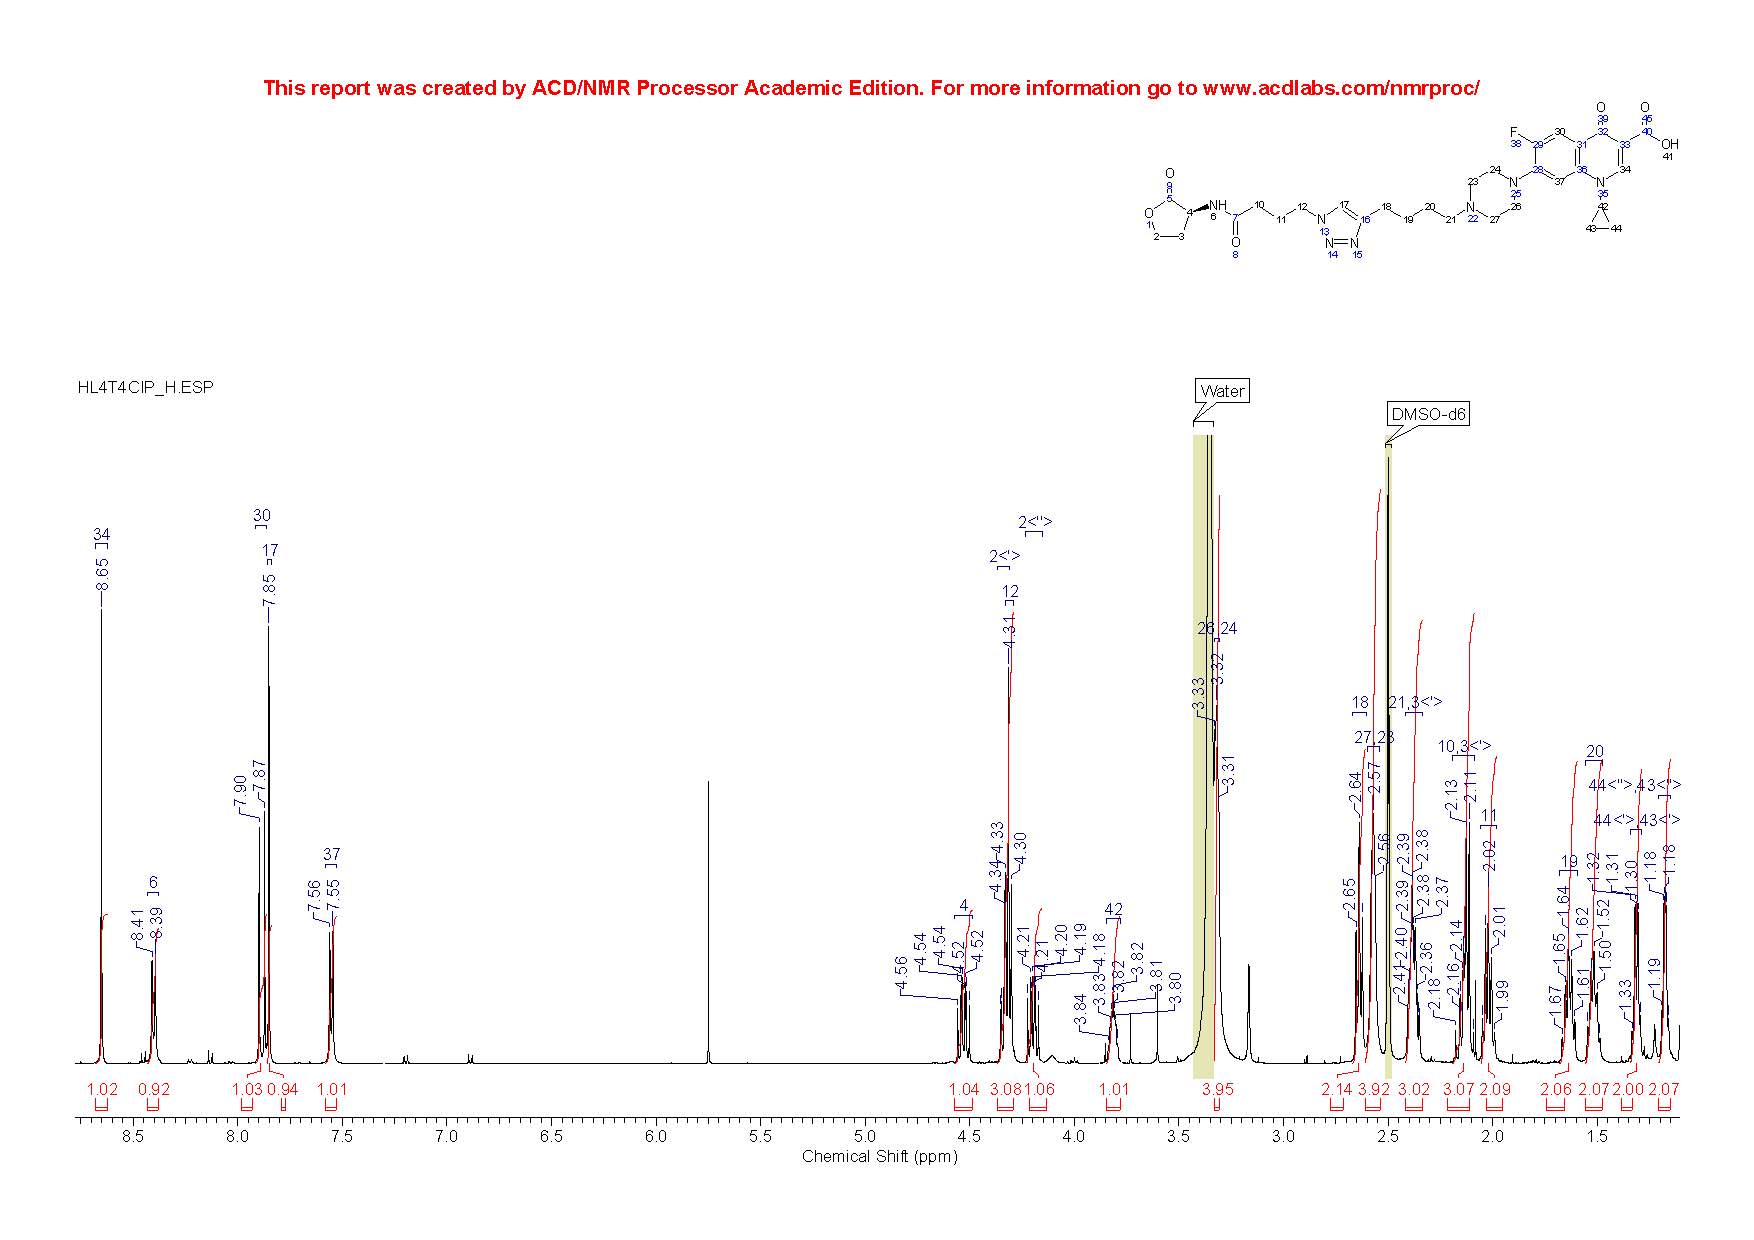
\includegraphics[ width=1.0\textwidth,height=0.43\textheight,keepaspectratio,trim={0 0 0 1.7cm},clip]{HL4T4Cip_H.pdf}
		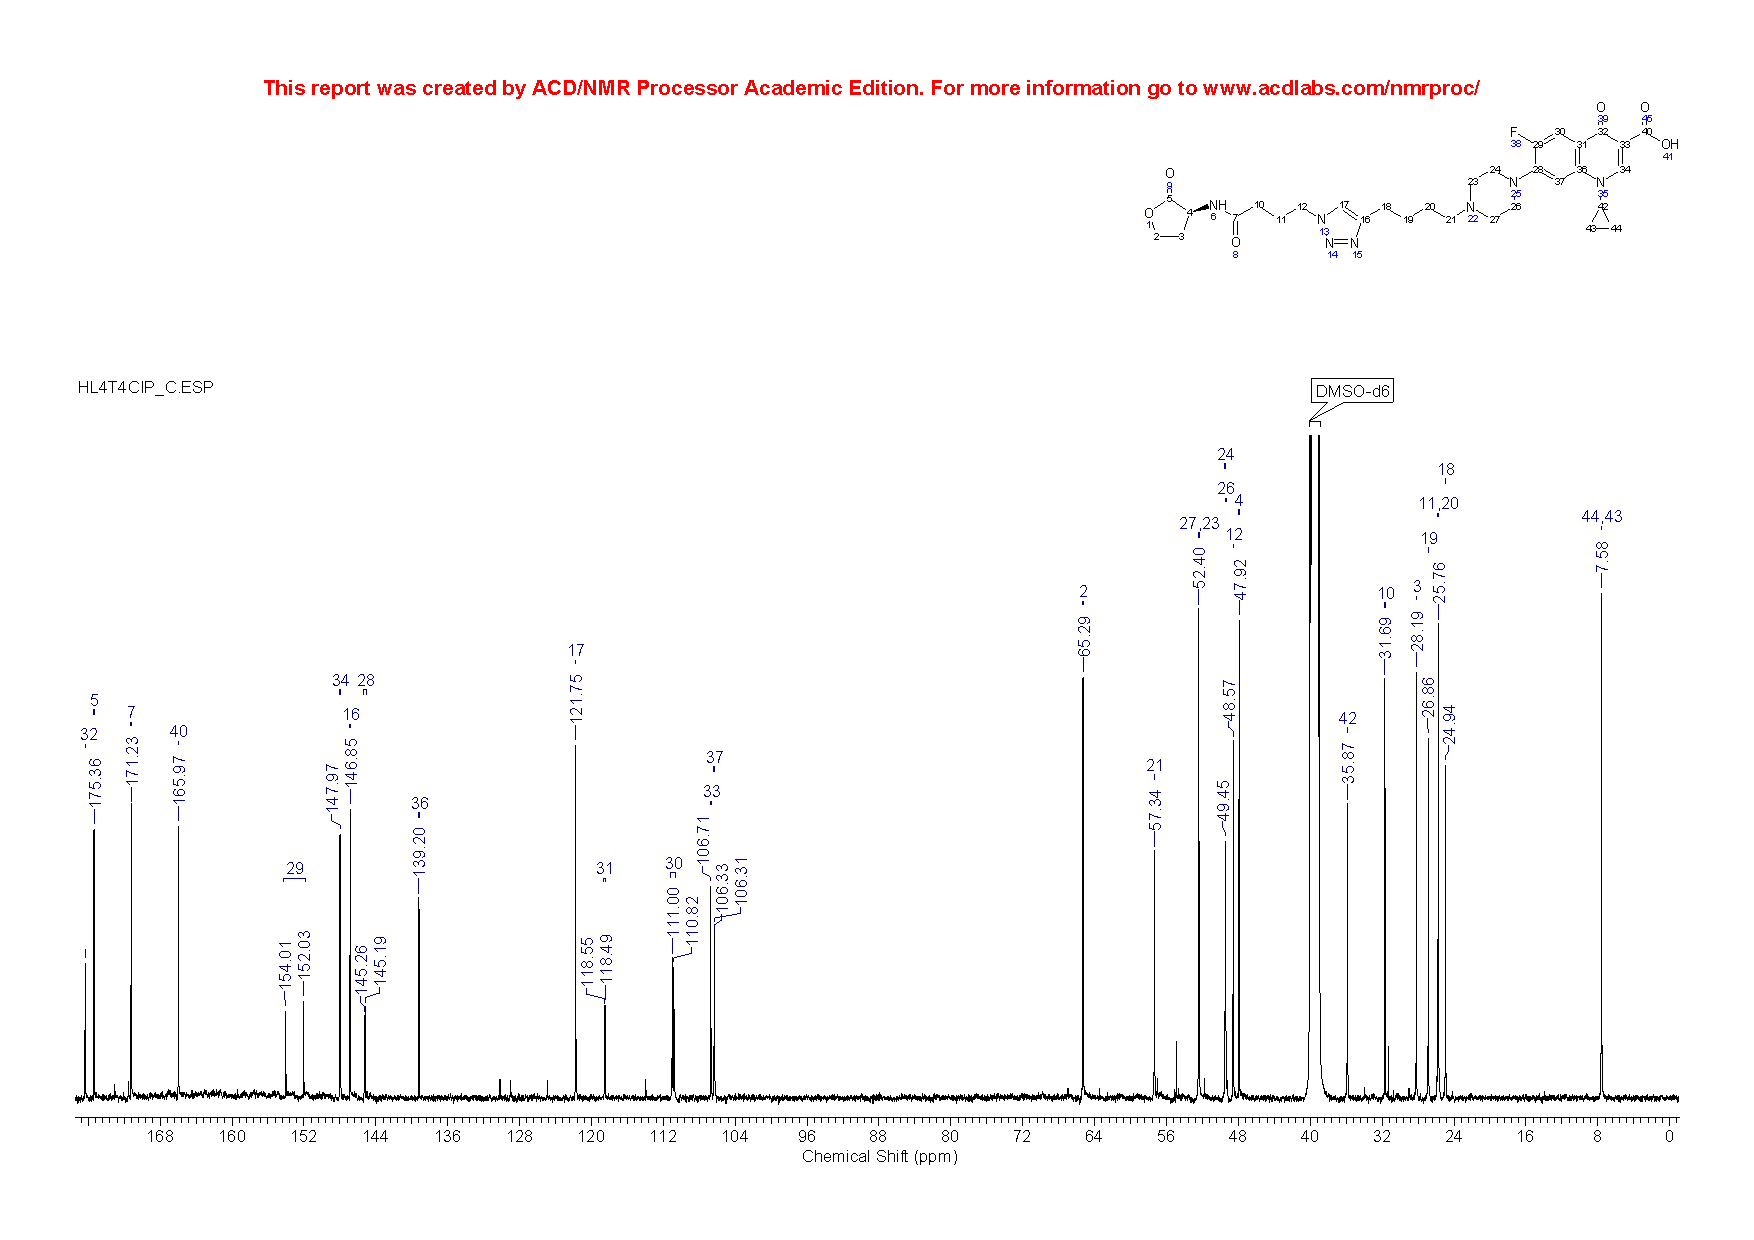
\includegraphics[ width=1.0\textwidth,height=0.43\textheight,keepaspectratio,trim={0 0 0 1.7cm},clip]{HL4T4Cip_C.pdf}
\end{figure}

\subsection{(\textit{S})-1-Cyclopropyl-6-fluoro-4-oxo-7-(4-(4-(1-(6-oxo-6-((2-oxotetrahydrofuran\allowbreak -3-yl)amino)hexyl)-1\textit{H}-1,2,3-triazol-4-yl)butyl)piperazin-1-yl)-1,4-dihydroqui\allowbreak n\allowbreak oline-3-carboxylic acid \compound{cmpd:HL6T4Cip}}

\begin{figure}[H]
	\centering
		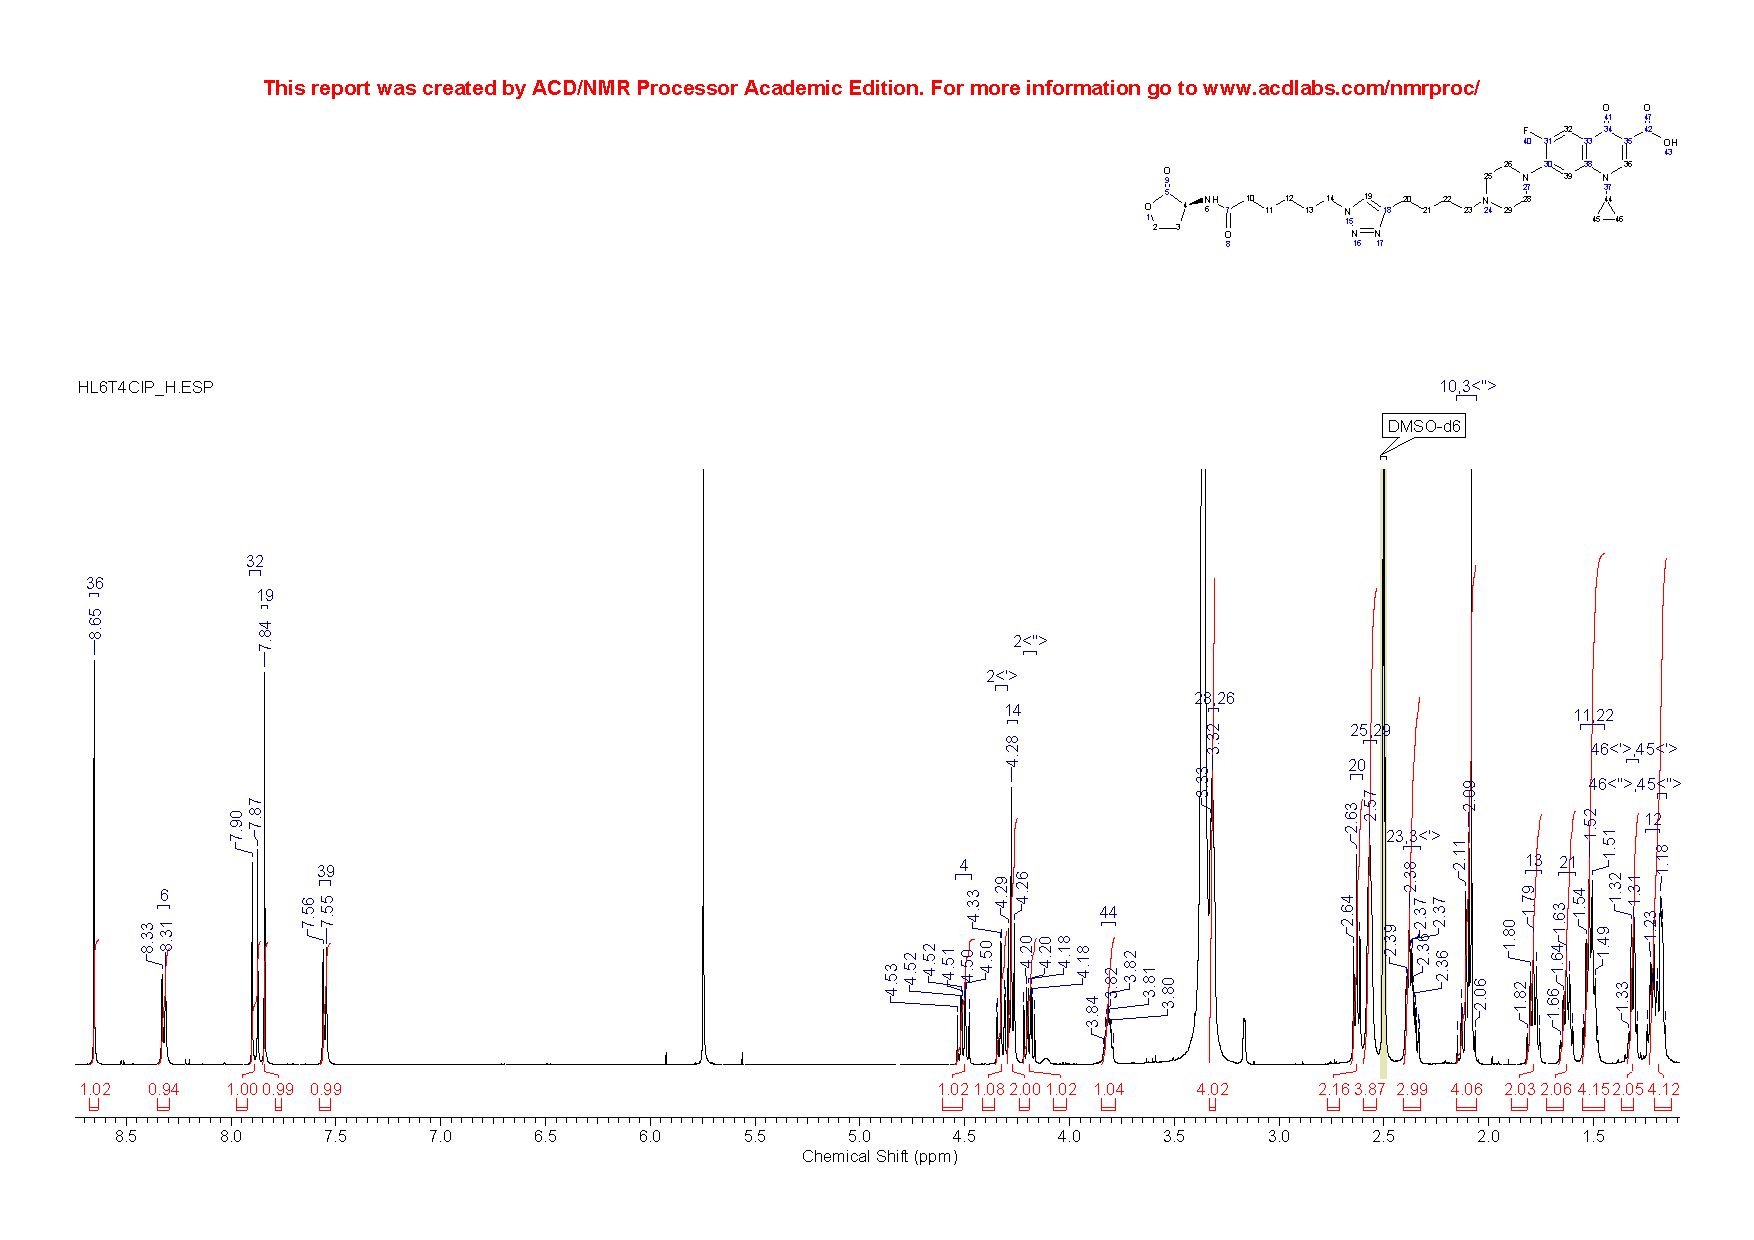
\includegraphics[ width=1.0\textwidth,height=0.43\textheight,keepaspectratio,trim={0 0 0 1.7cm},clip]{HL6T4Cip_H.pdf}
		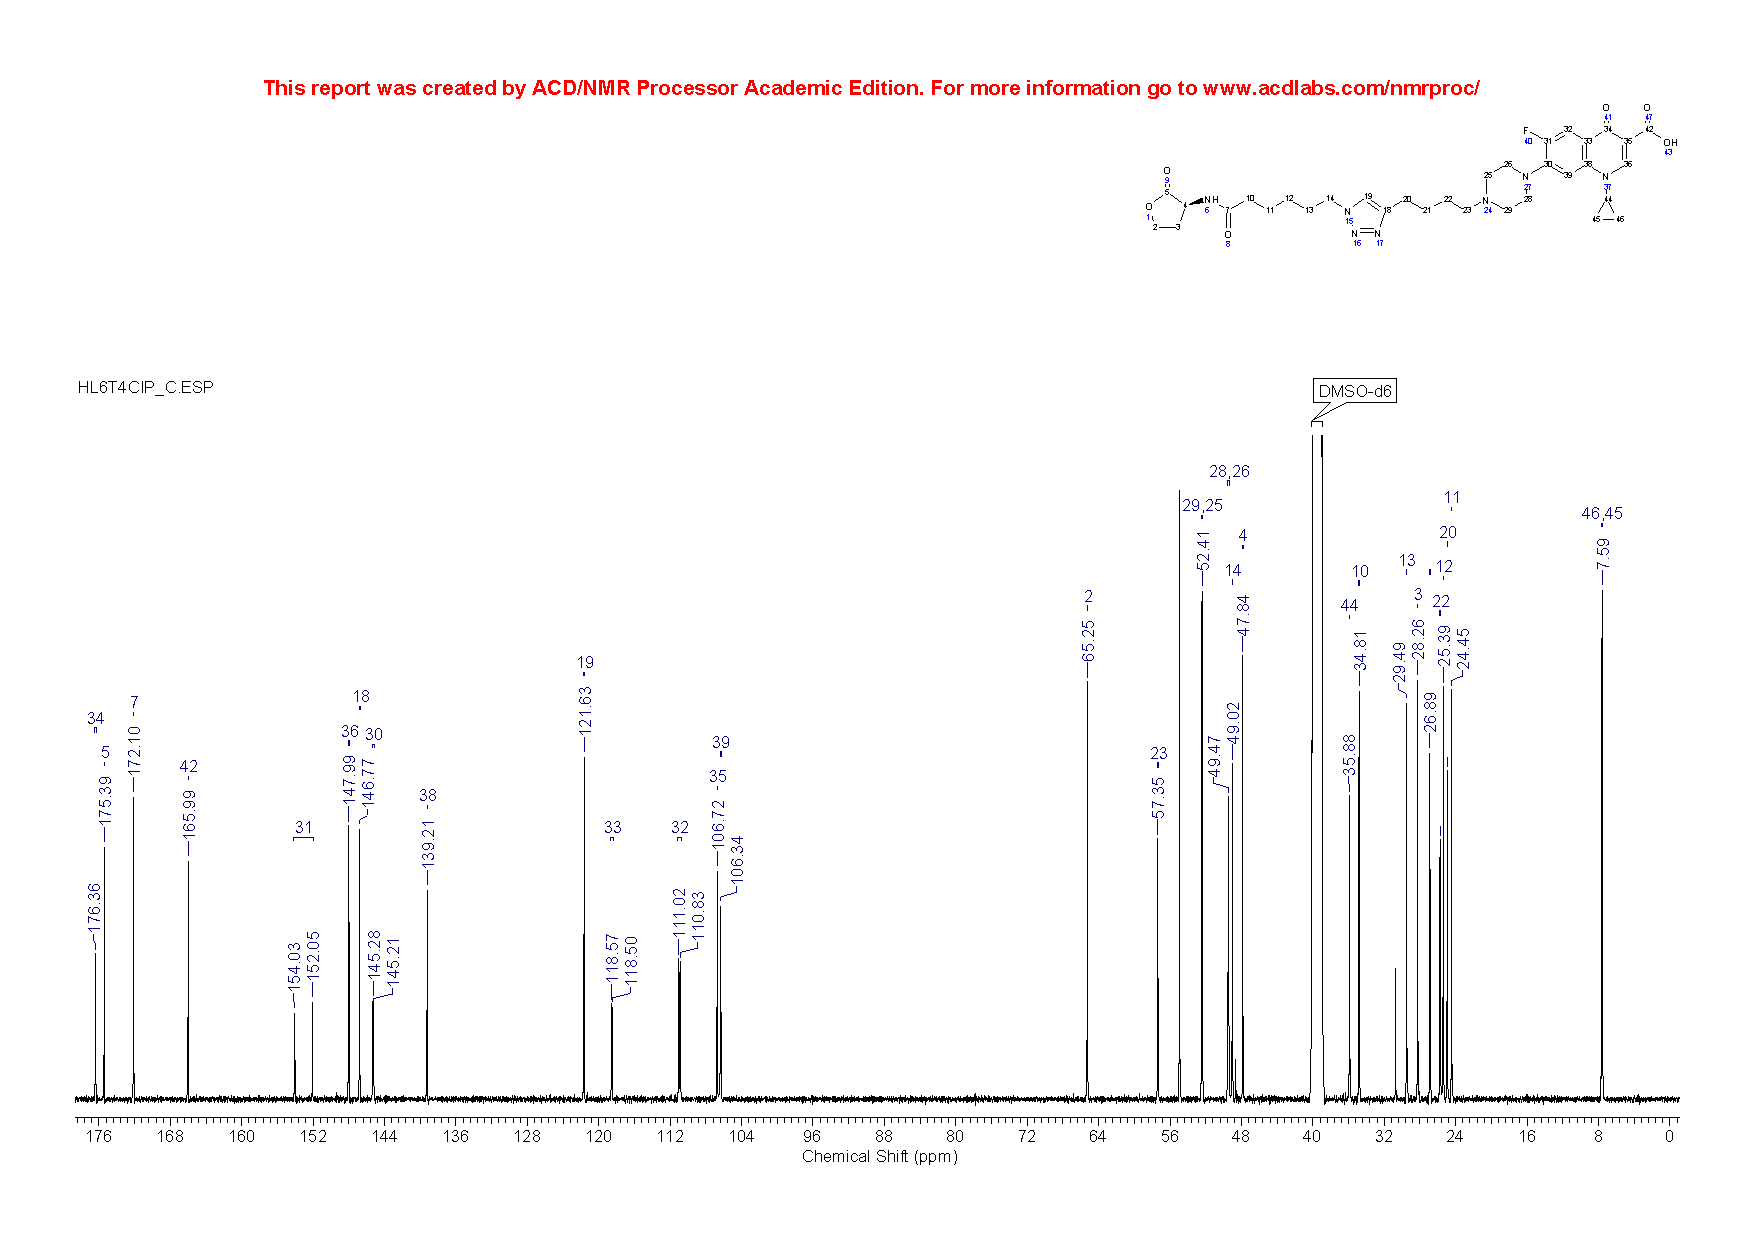
\includegraphics[ width=1.0\textwidth,height=0.43\textheight,keepaspectratio,trim={0 0 0 1.7cm},clip]{HL6T4Cip_C.pdf}
\end{figure}

\subsection{1-Cyclopropyl-6-fluoro-7-(4-(4-(1-(2-heptyl-4-oxo-1,4-dihydroquinolin-6-yl)-1\allowbreak \textit{H}-1,2,3-triazol-4-yl)\allowbreak bu\allowbreak tyl)piperazin-1-yl)-4-oxo-1,4-dihydroqui\allowbreak n\allowbreak oline-3-carbo\allowbreak xylic acid \compound{cmpd:6HHQT4Cip}}

\begin{figure}[H]
	\centering
		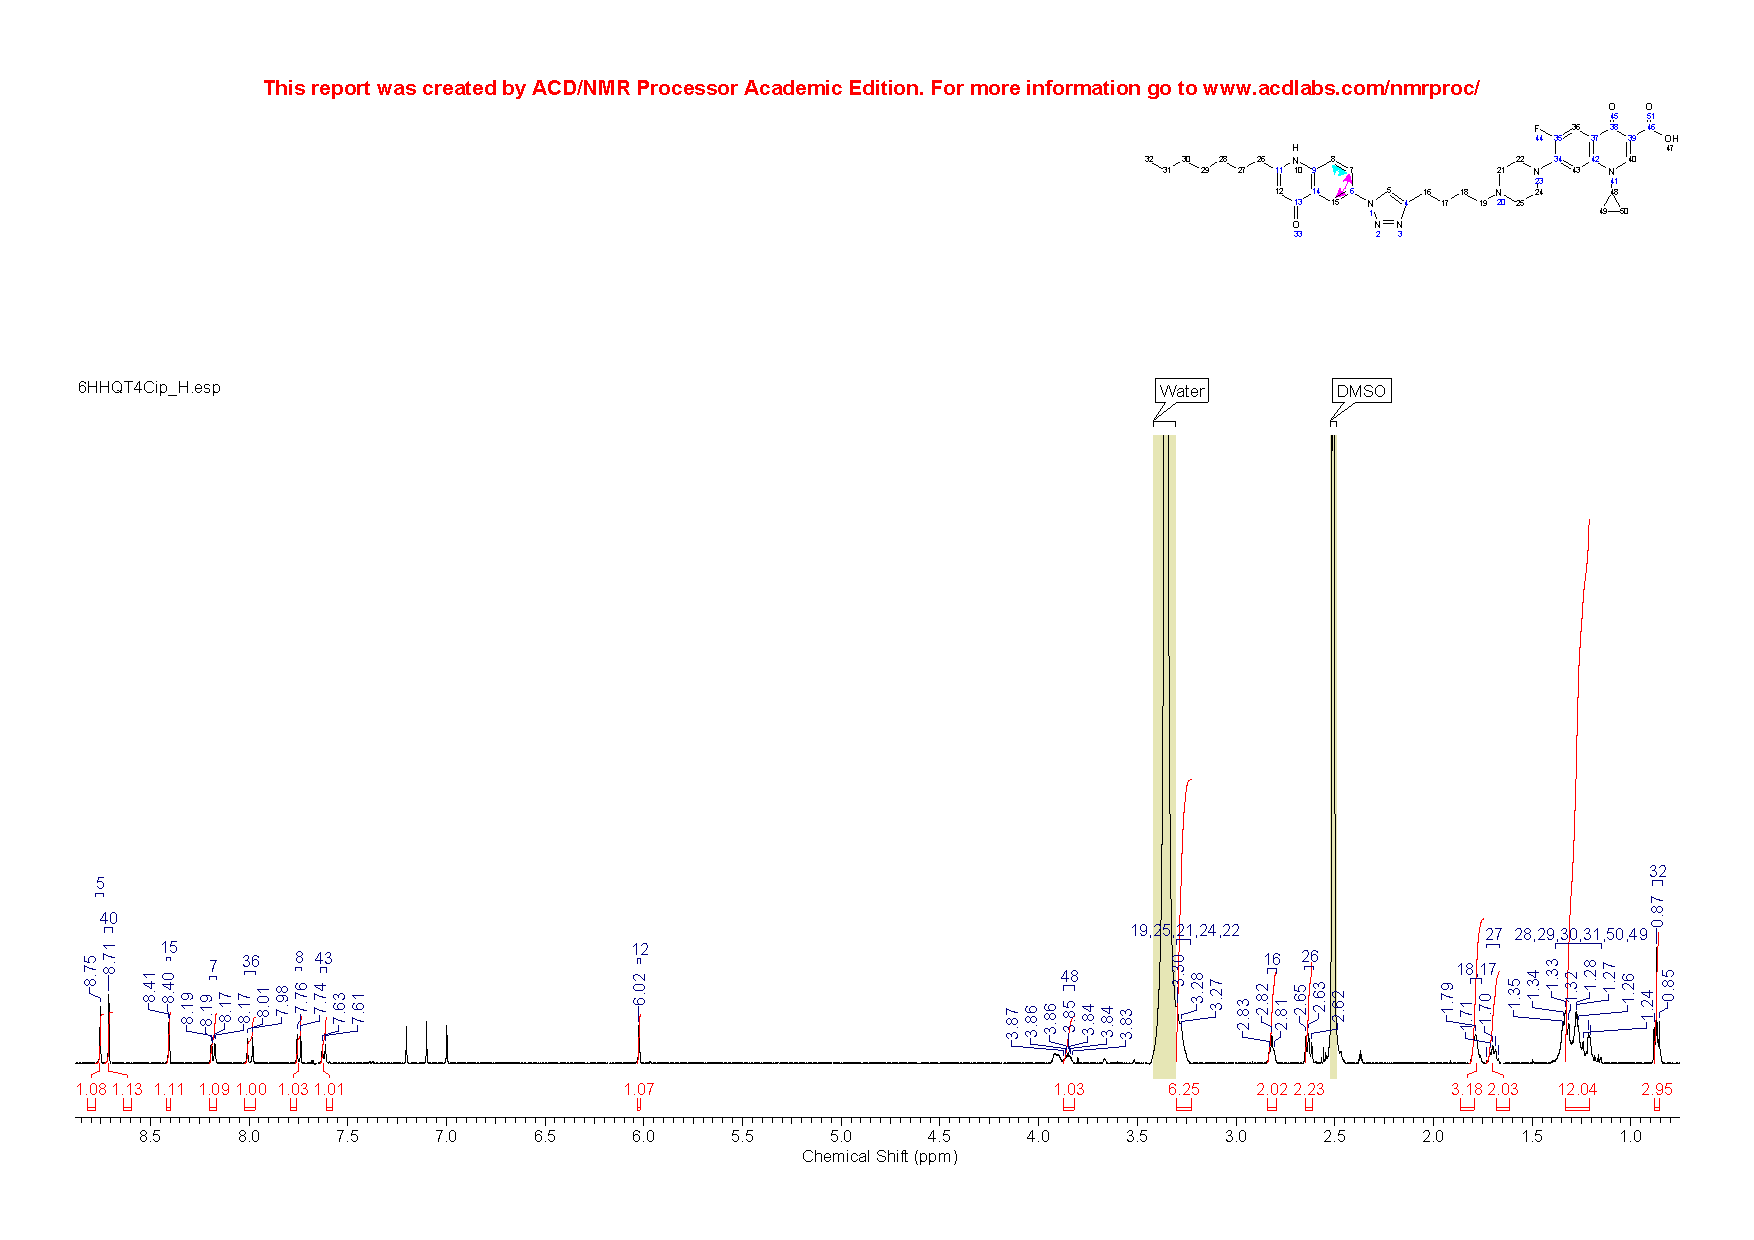
\includegraphics[ width=1.0\textwidth,height=0.43\textheight,keepaspectratio,trim={0 0 0 1.7cm},clip]{6HHQT4Cip_H.pdf}
		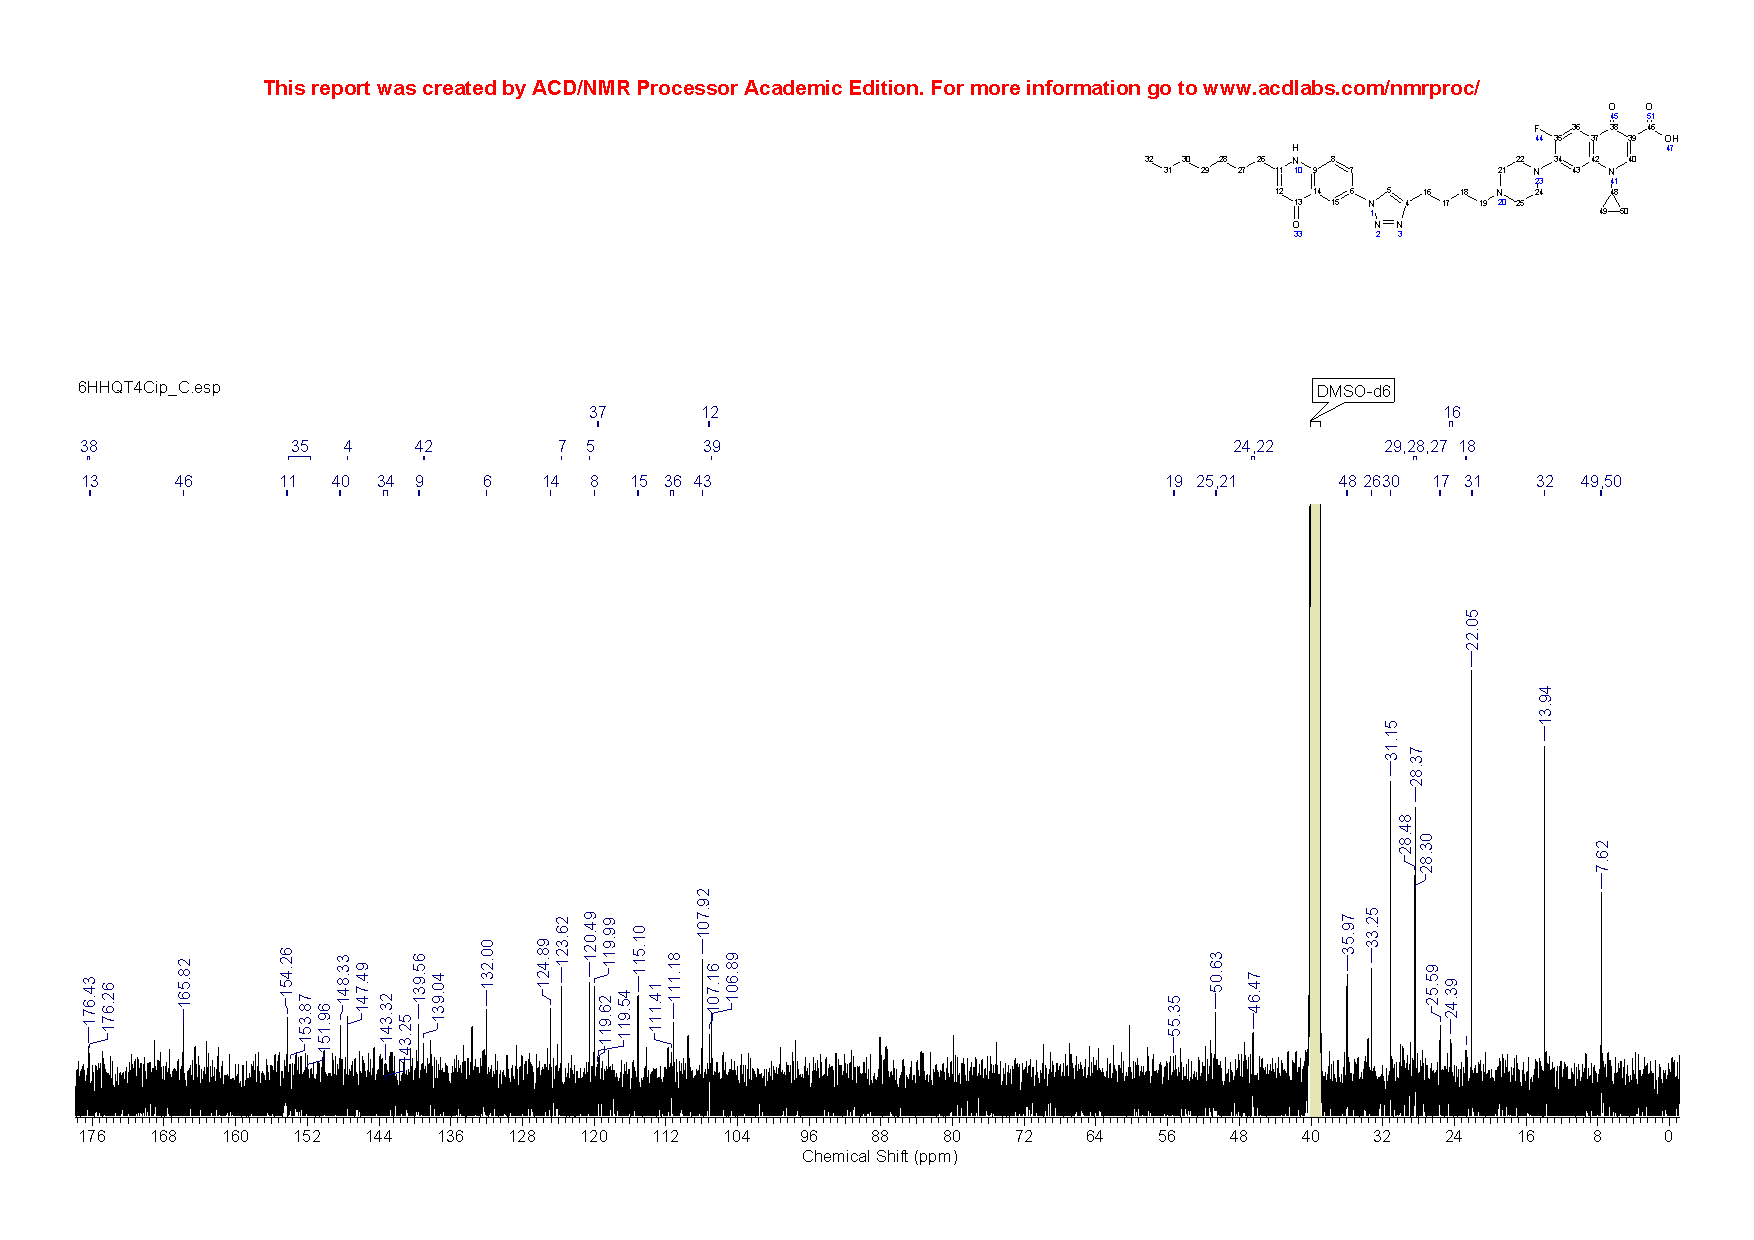
\includegraphics[ width=1.0\textwidth,height=0.43\textheight,keepaspectratio,trim={0 0 0 1.7cm},clip]{6HHQT4Cip_C.pdf}
\end{figure}

\subsection{(\textit{S})-4-(4-(4-(4-((2,4-Diaminopyrimidin-5-yl)methyl)-2,6-dimethoxyphenoxy)\allowbreak bu\allowbreak tyl)-1\textit{H}-1,2,3-triazol-1-yl)-\textit{N}-(2-oxotetrahydrofuran-3-yl)butanamide \compound{cmpd:HL4T4Tri}}

\begin{figure}[H]
	\centering
		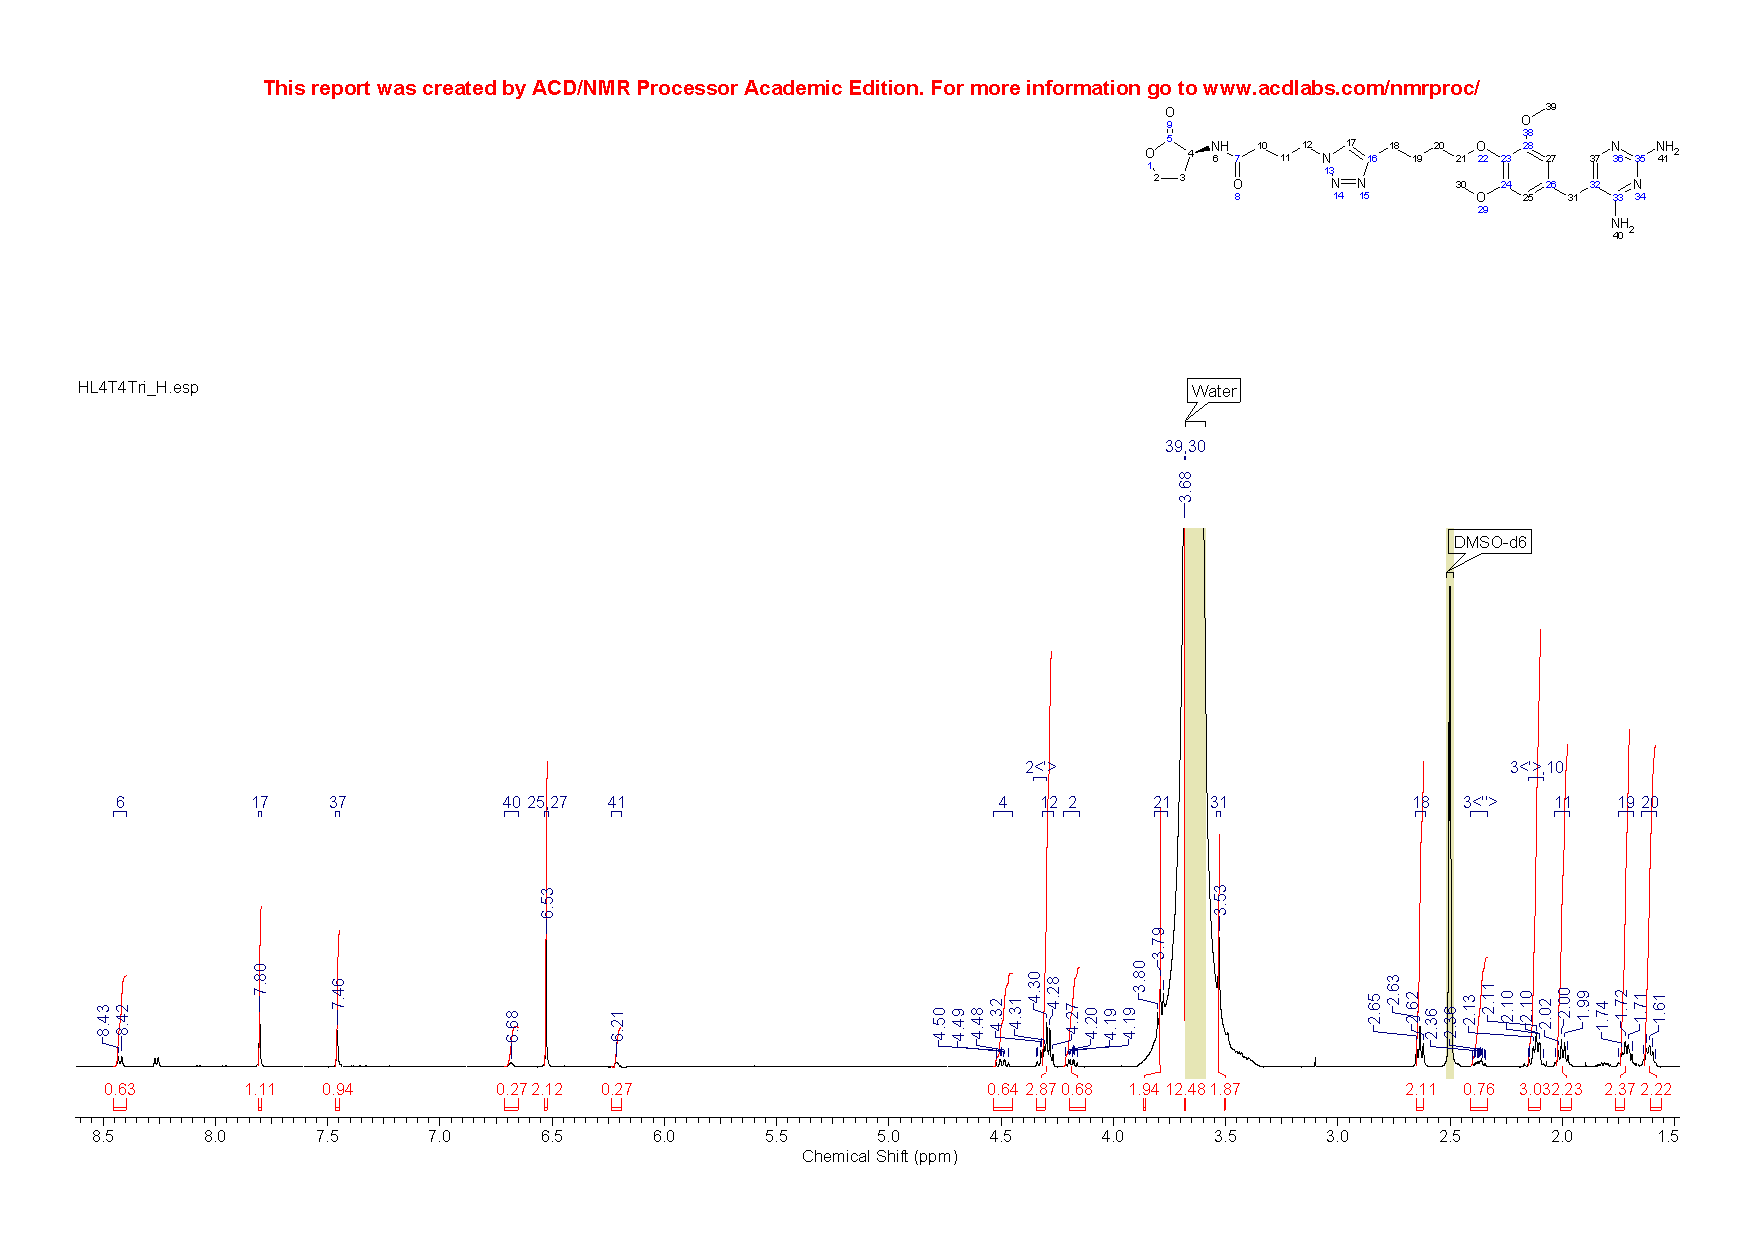
\includegraphics[ width=1.0\textwidth,height=0.43\textheight,keepaspectratio,trim={0 0 0 1.7cm},clip]{HL4T4Tri_H.pdf}
		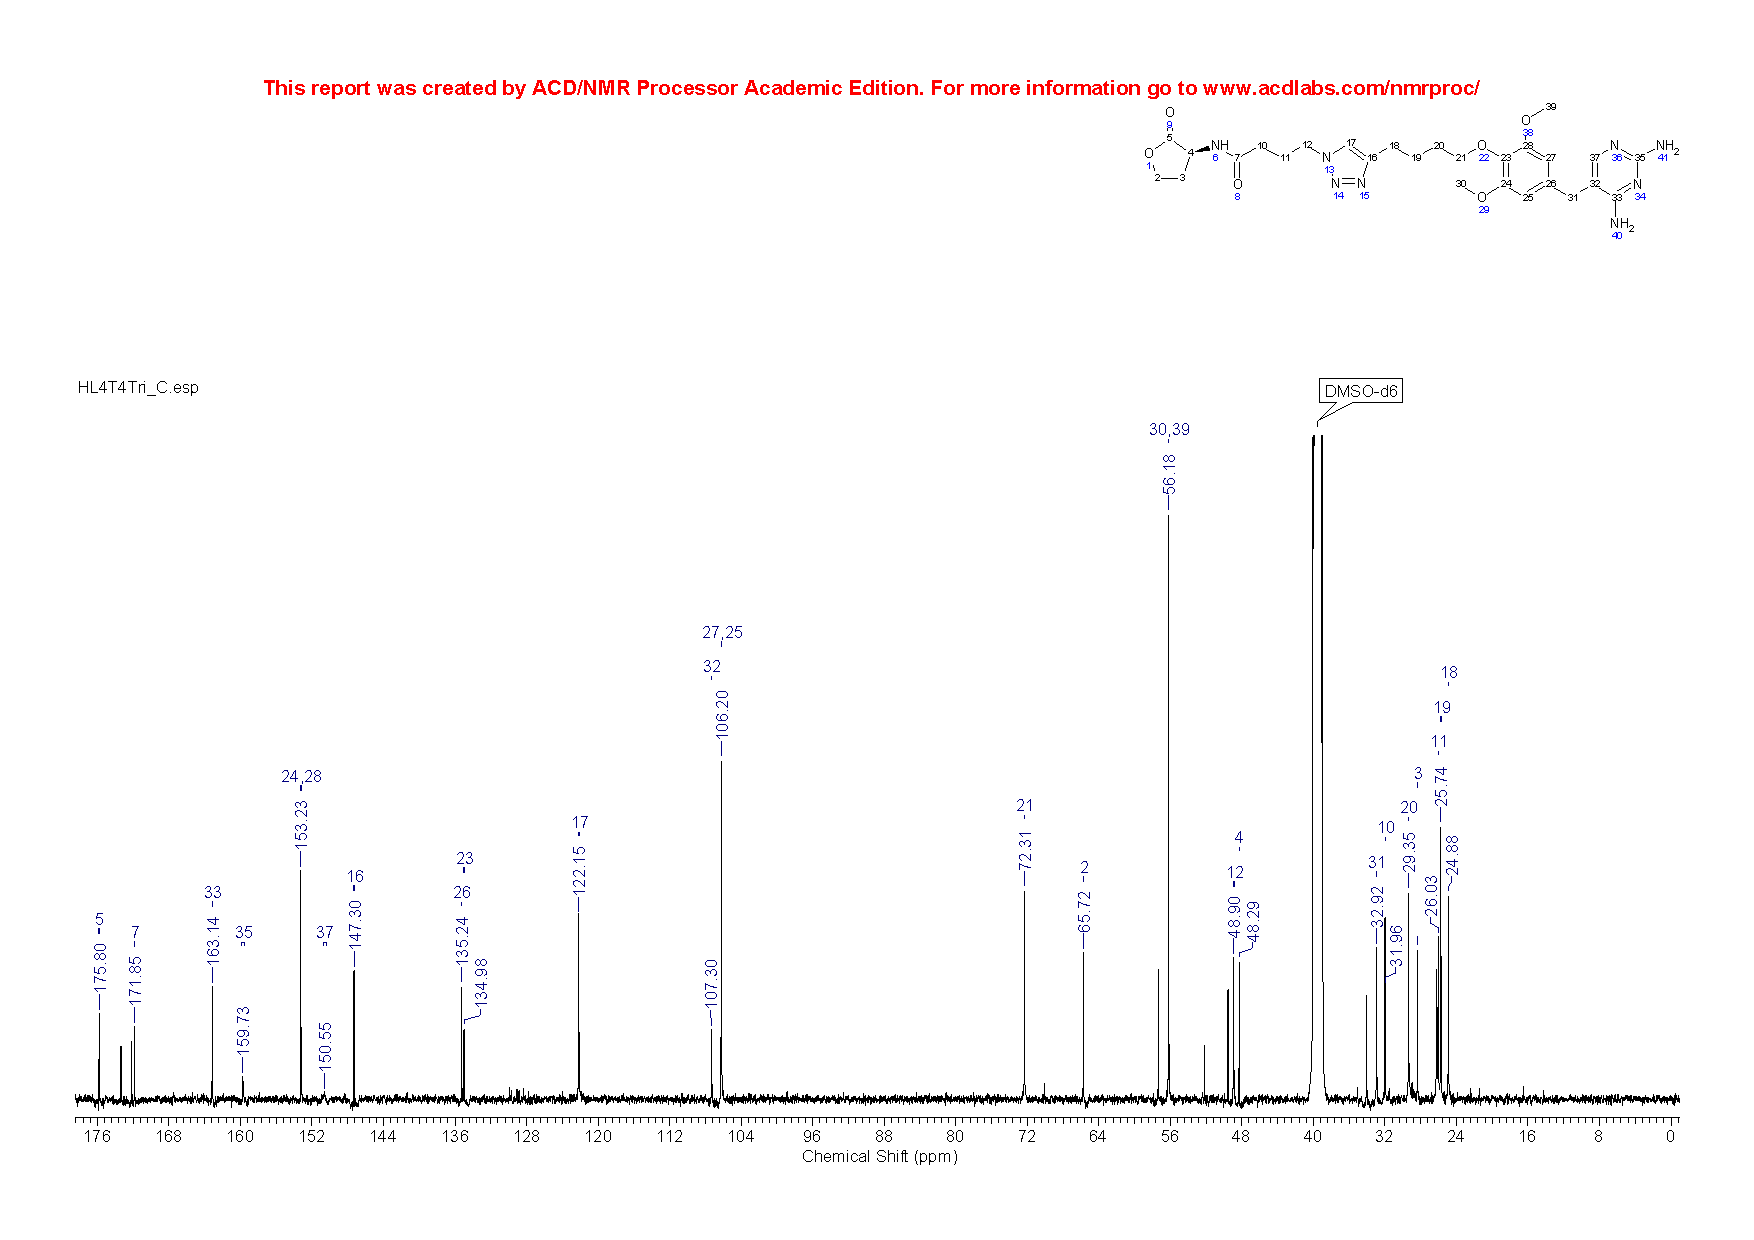
\includegraphics[ width=1.0\textwidth,height=0.43\textheight,keepaspectratio,trim={0 0 0 1.7cm},clip]{HL4T4Tri_C.pdf}
\end{figure}

\subsection{(\textit{S})-6-(4-(4-(4-((2,4-Diaminopyrimidin-5-yl)methyl)-2,6-dimethoxyphenoxy)bu\allowbreak tyl)-1\textit{H}-1,2,3-triazol-1-yl)-\textit{N}-(2-oxotetrahydrofuran-3-yl)hexanamide \compound{cmpd:HL6T4Tri}}

\begin{figure}[H]
	\centering
		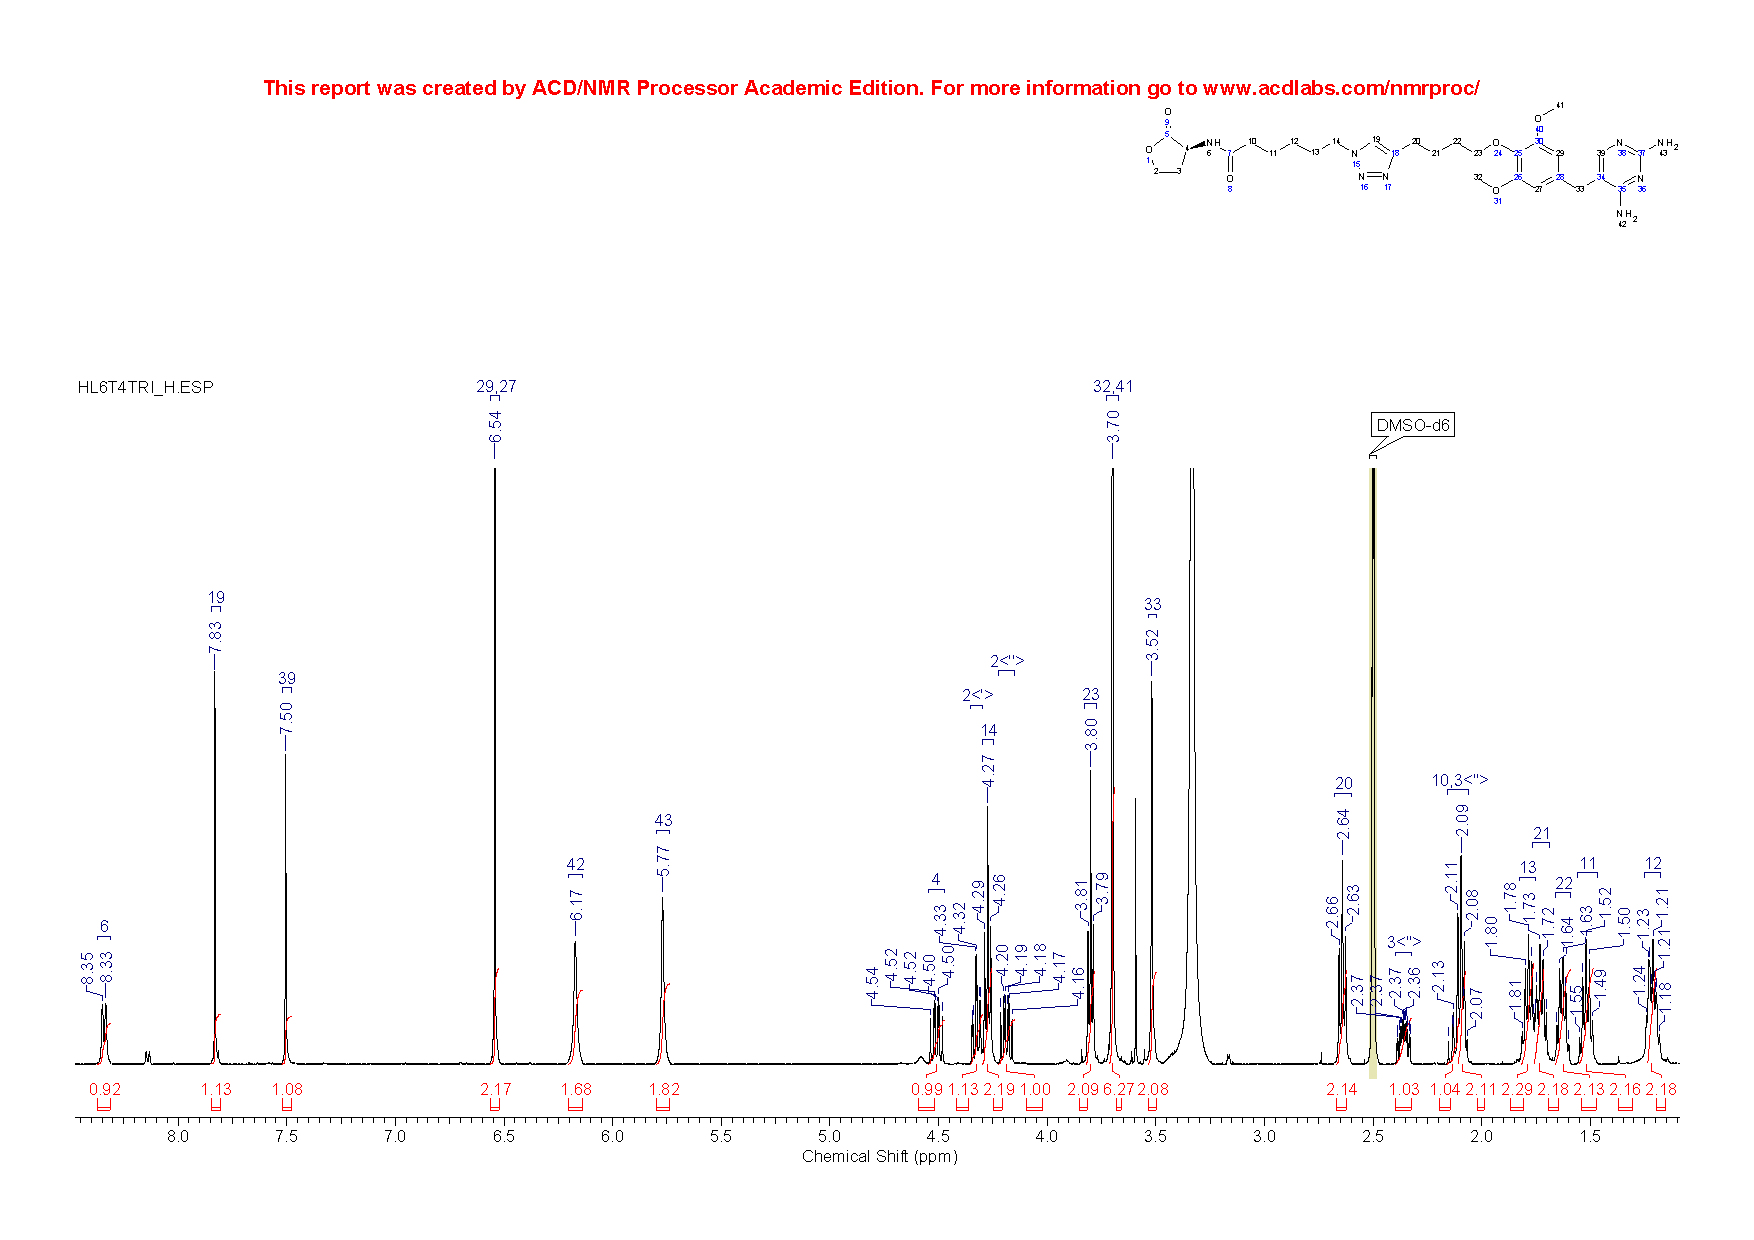
\includegraphics[ width=1.0\textwidth,height=0.43\textheight,keepaspectratio,trim={0 0 0 1.7cm},clip]{HL6T4Tri_H.pdf}
		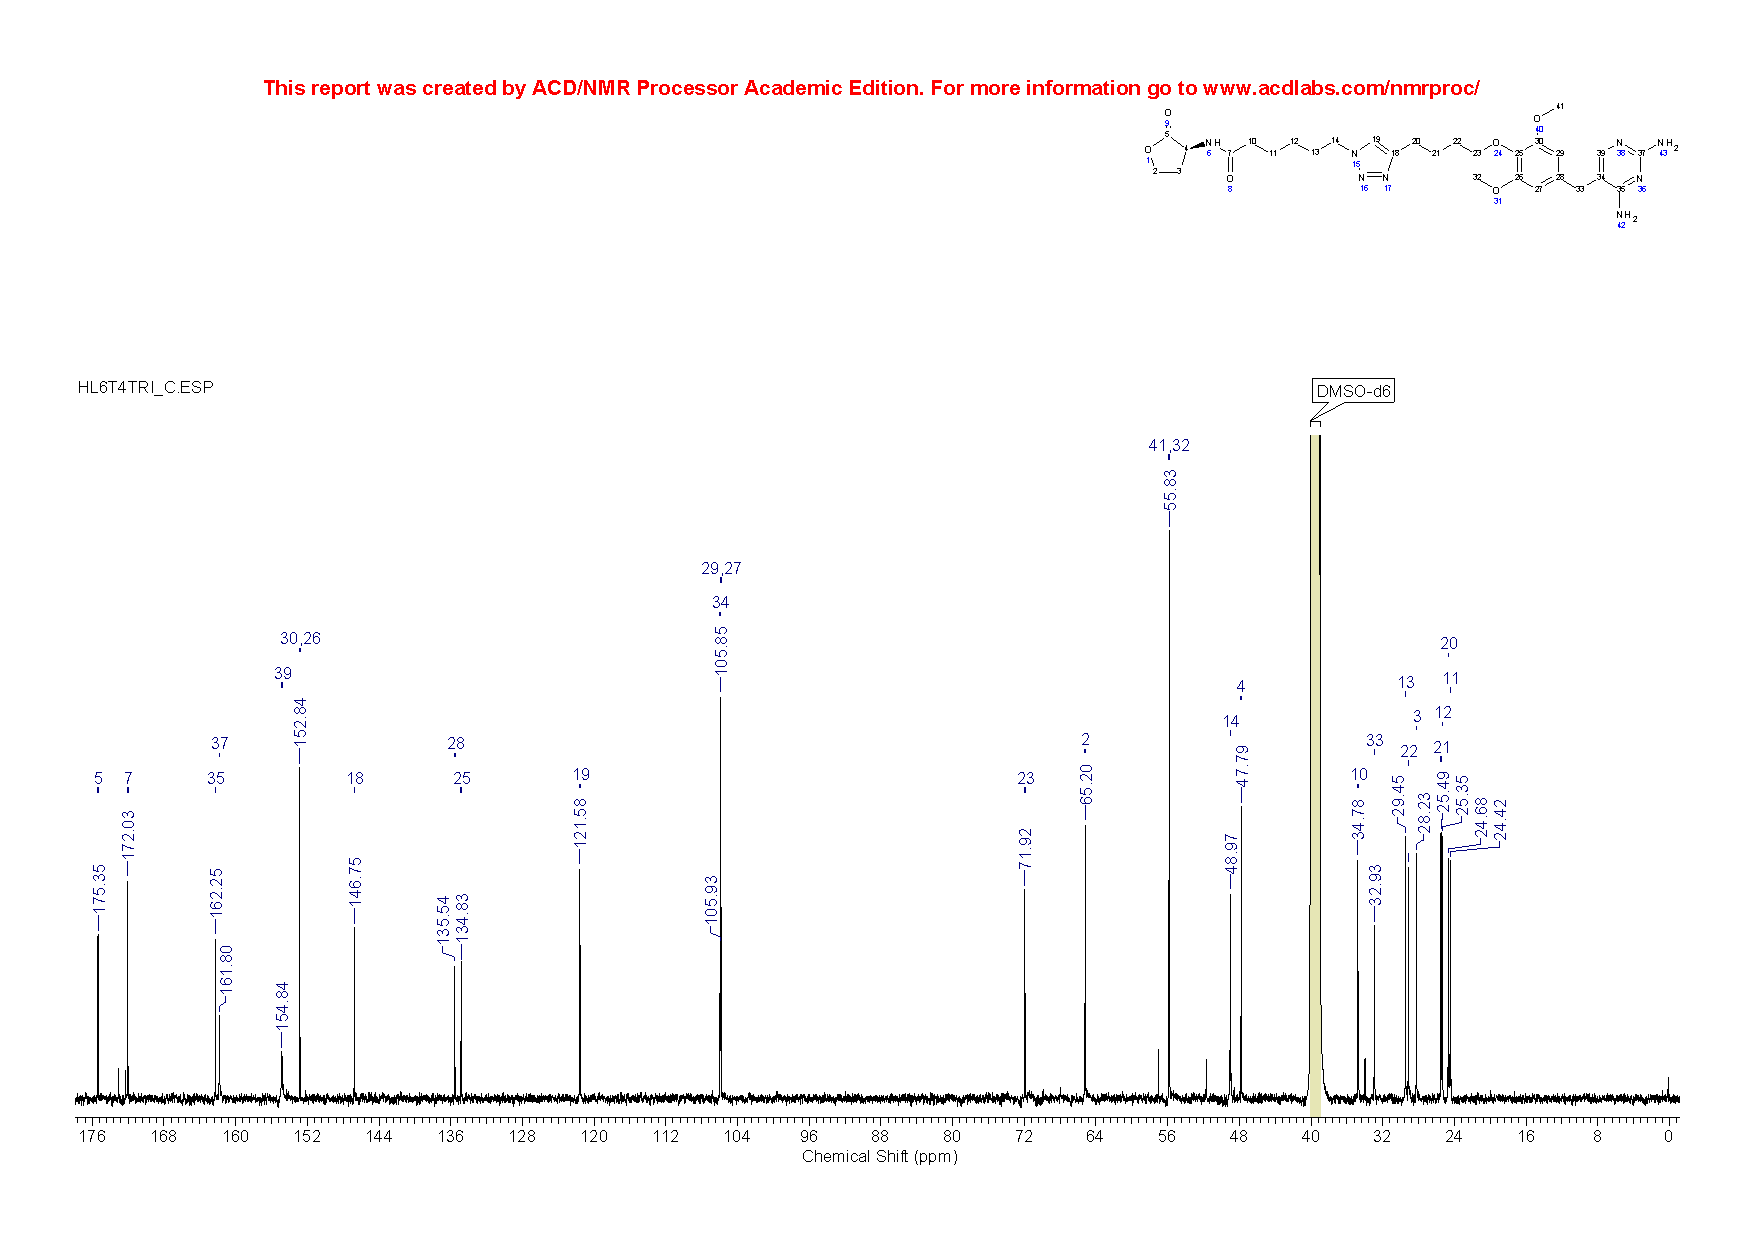
\includegraphics[ width=1.0\textwidth,height=0.43\textheight,keepaspectratio,trim={0 0 0 1.7cm},clip]{HL6T4Tri_C.pdf}
\end{figure}

\subsection{6-(4-(4-(4-((2,4-Diaminopyrimidin-5-yl)methyl)-2,6-dimethoxyphenoxy)butyl)\allowbreak -1\textit{H}-1,2,3-triazol-1-yl)-2-heptylquinolin-4(1\textit{H})-one \compound{cmpd:6HHQT4Tri}}

\begin{figure}[H]
	\centering
		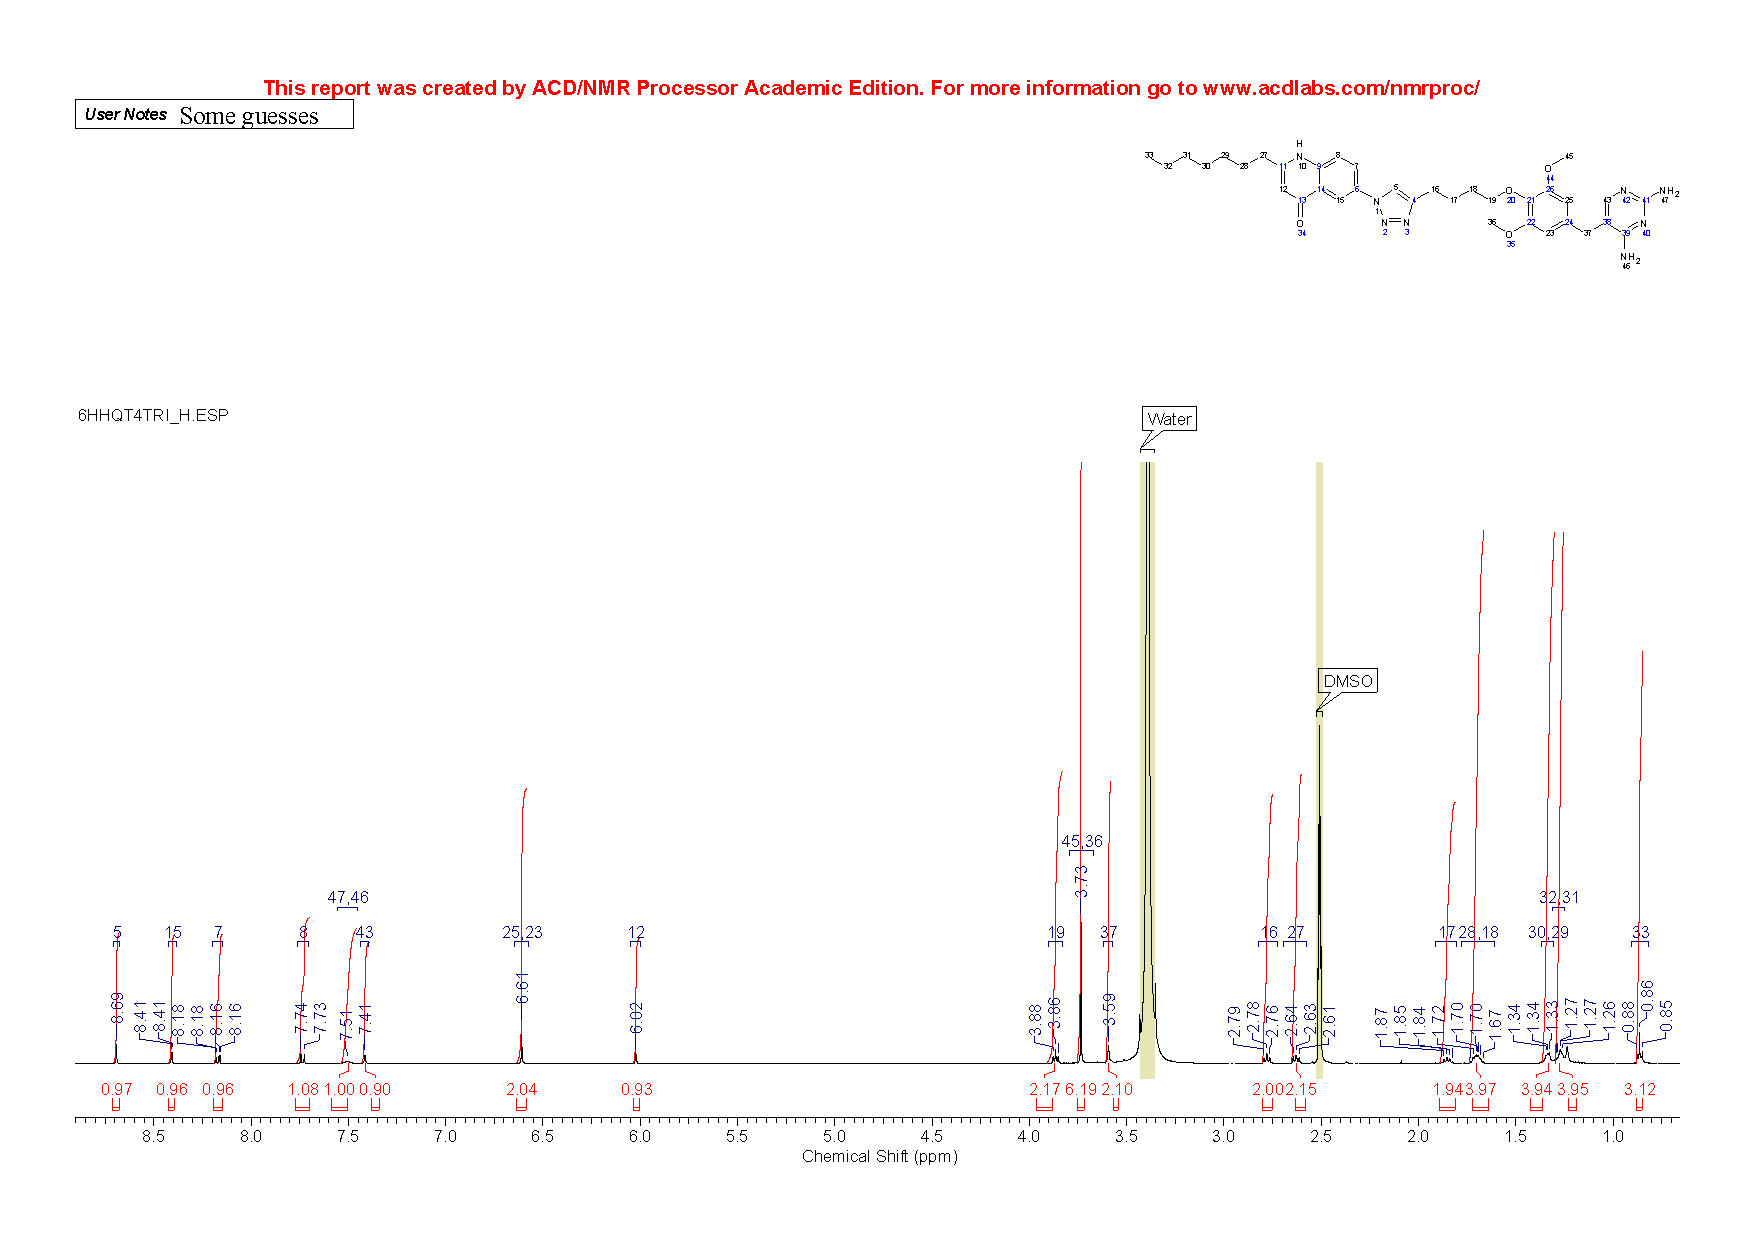
\includegraphics[ width=1.0\textwidth,height=0.43\textheight,keepaspectratio,trim={0 0 0 1.7cm},clip]{6HHQT4Tri_H.pdf}
		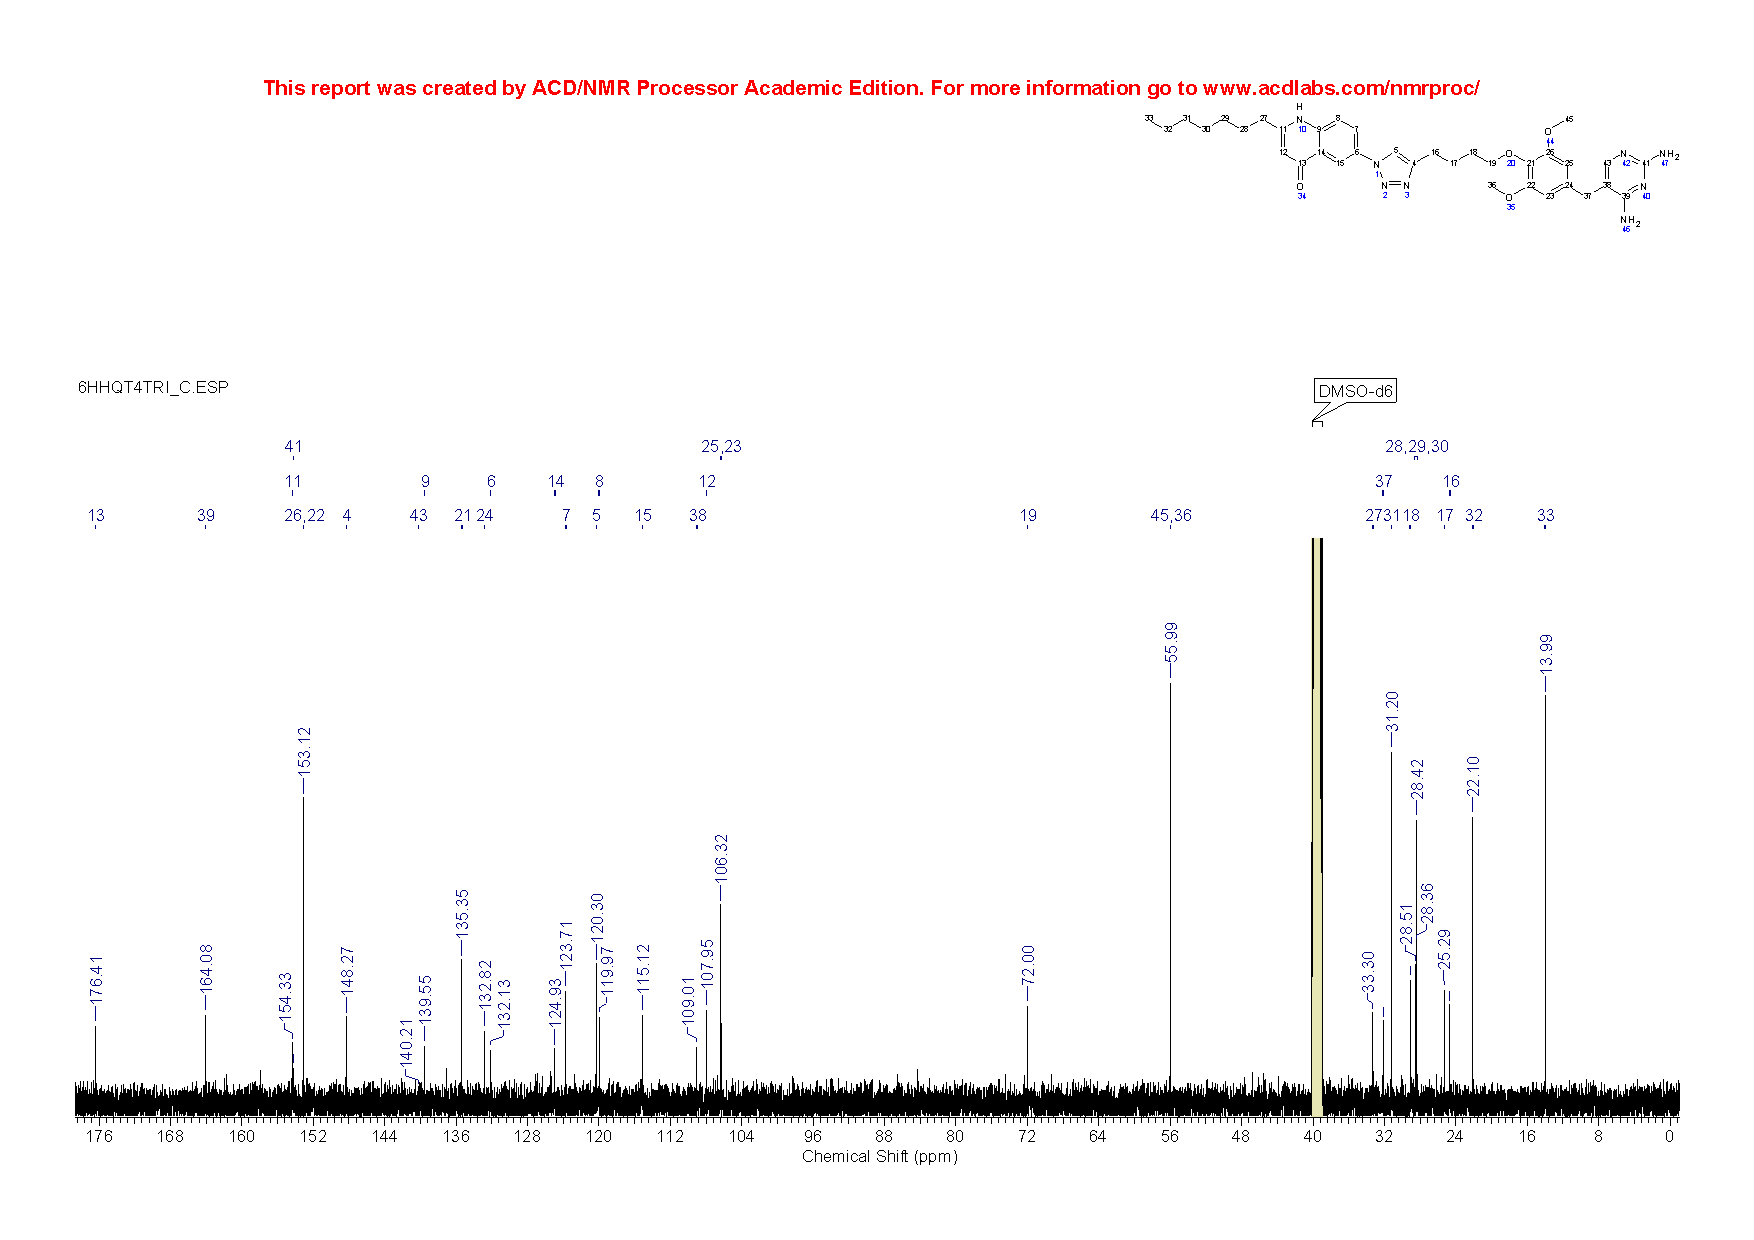
\includegraphics[ width=1.0\textwidth,height=0.43\textheight,keepaspectratio,trim={0 0 0 1.7cm},clip]{6HHQT4Tri_C.pdf}
\end{figure}

\subsection{2-(6-(4-(4-(4-((2,4-Diaminopyrimidin-5-yl)methyl)-2,6-dimethoxyphenoxy)bu\allowbreak tyl)-1\textit{H}-1,2,3-triazol-1-yl)hexyl)-3-hydroxyquinolin-4(1\textit{H})-one \compound{cmpd:PQST4Tri}}

\begin{figure}[H]
	\centering
		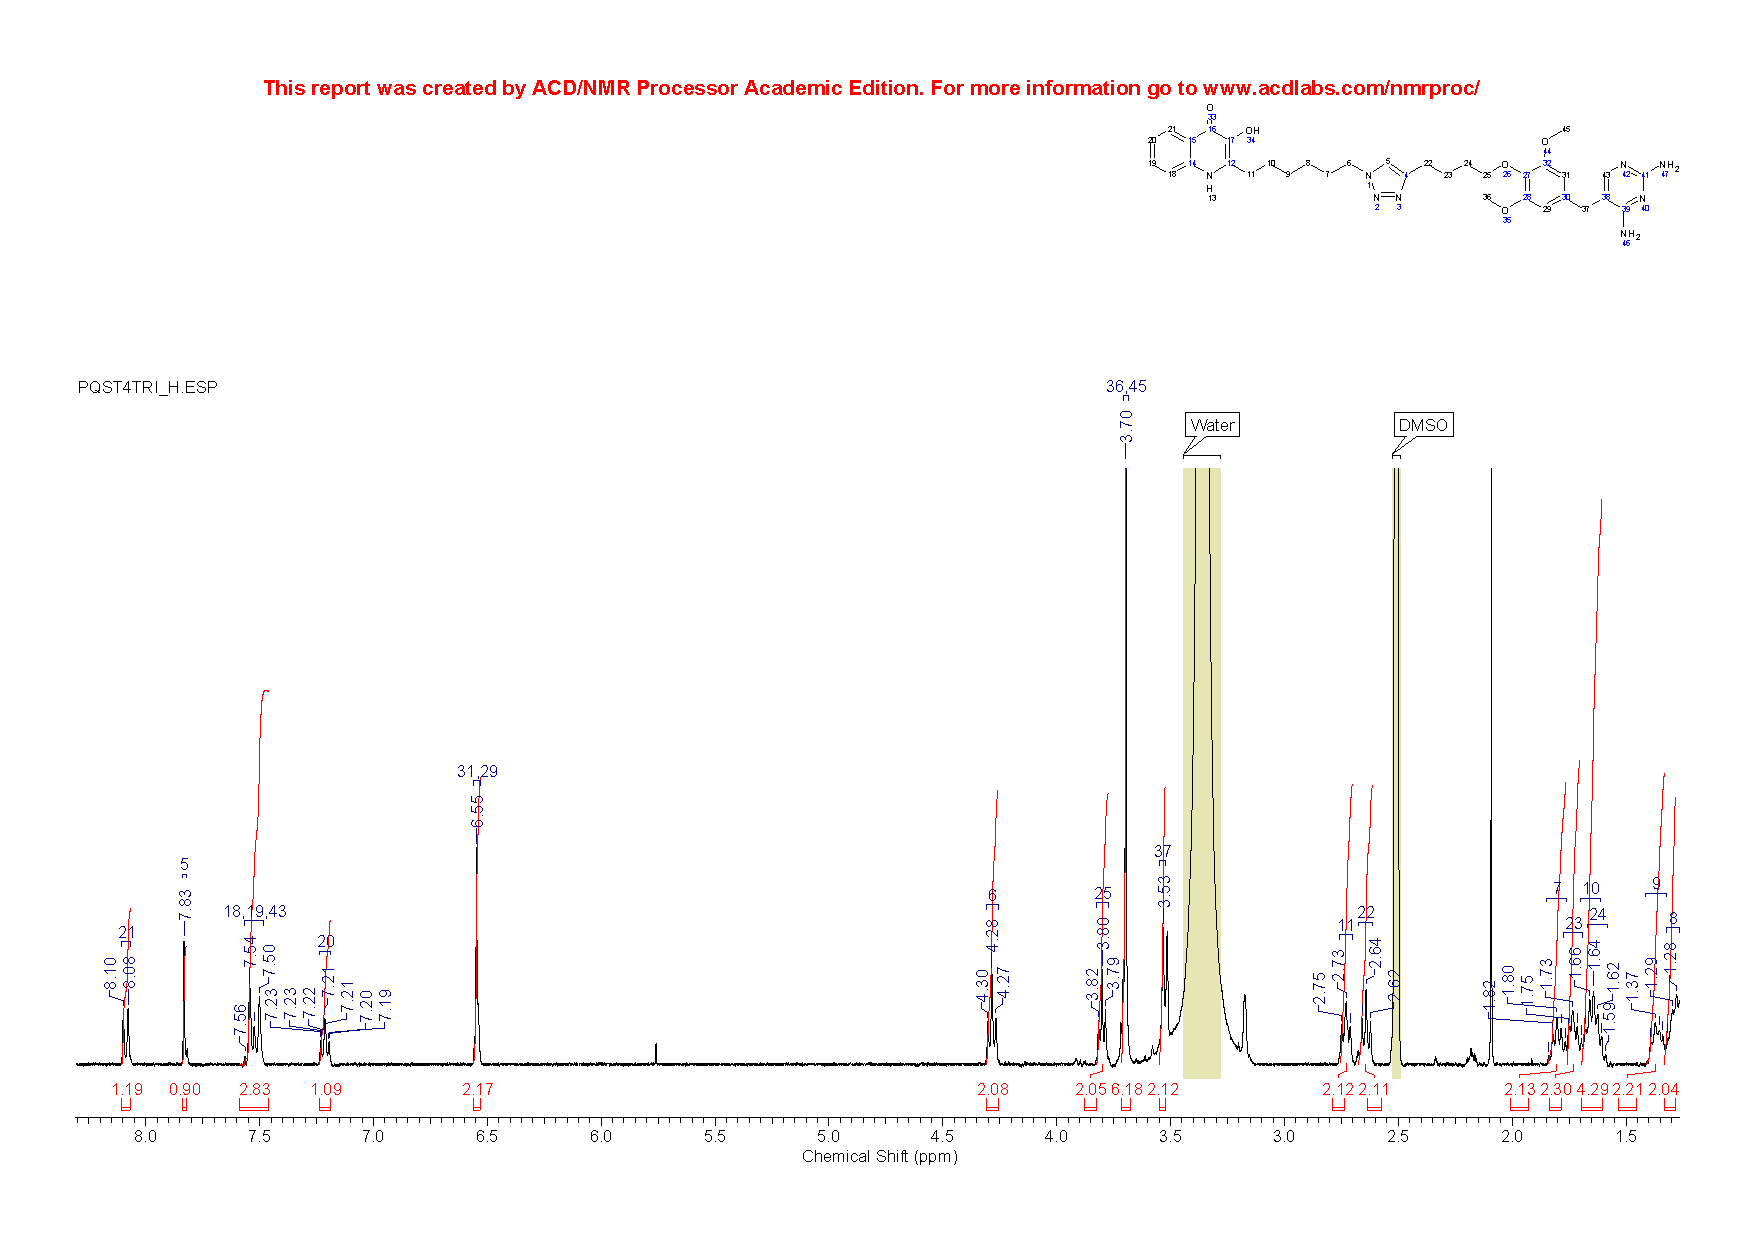
\includegraphics[ width=1.0\textwidth,height=0.43\textheight,keepaspectratio,trim={0 0 0 1.7cm},clip]{PQST4Tri_H.pdf}
		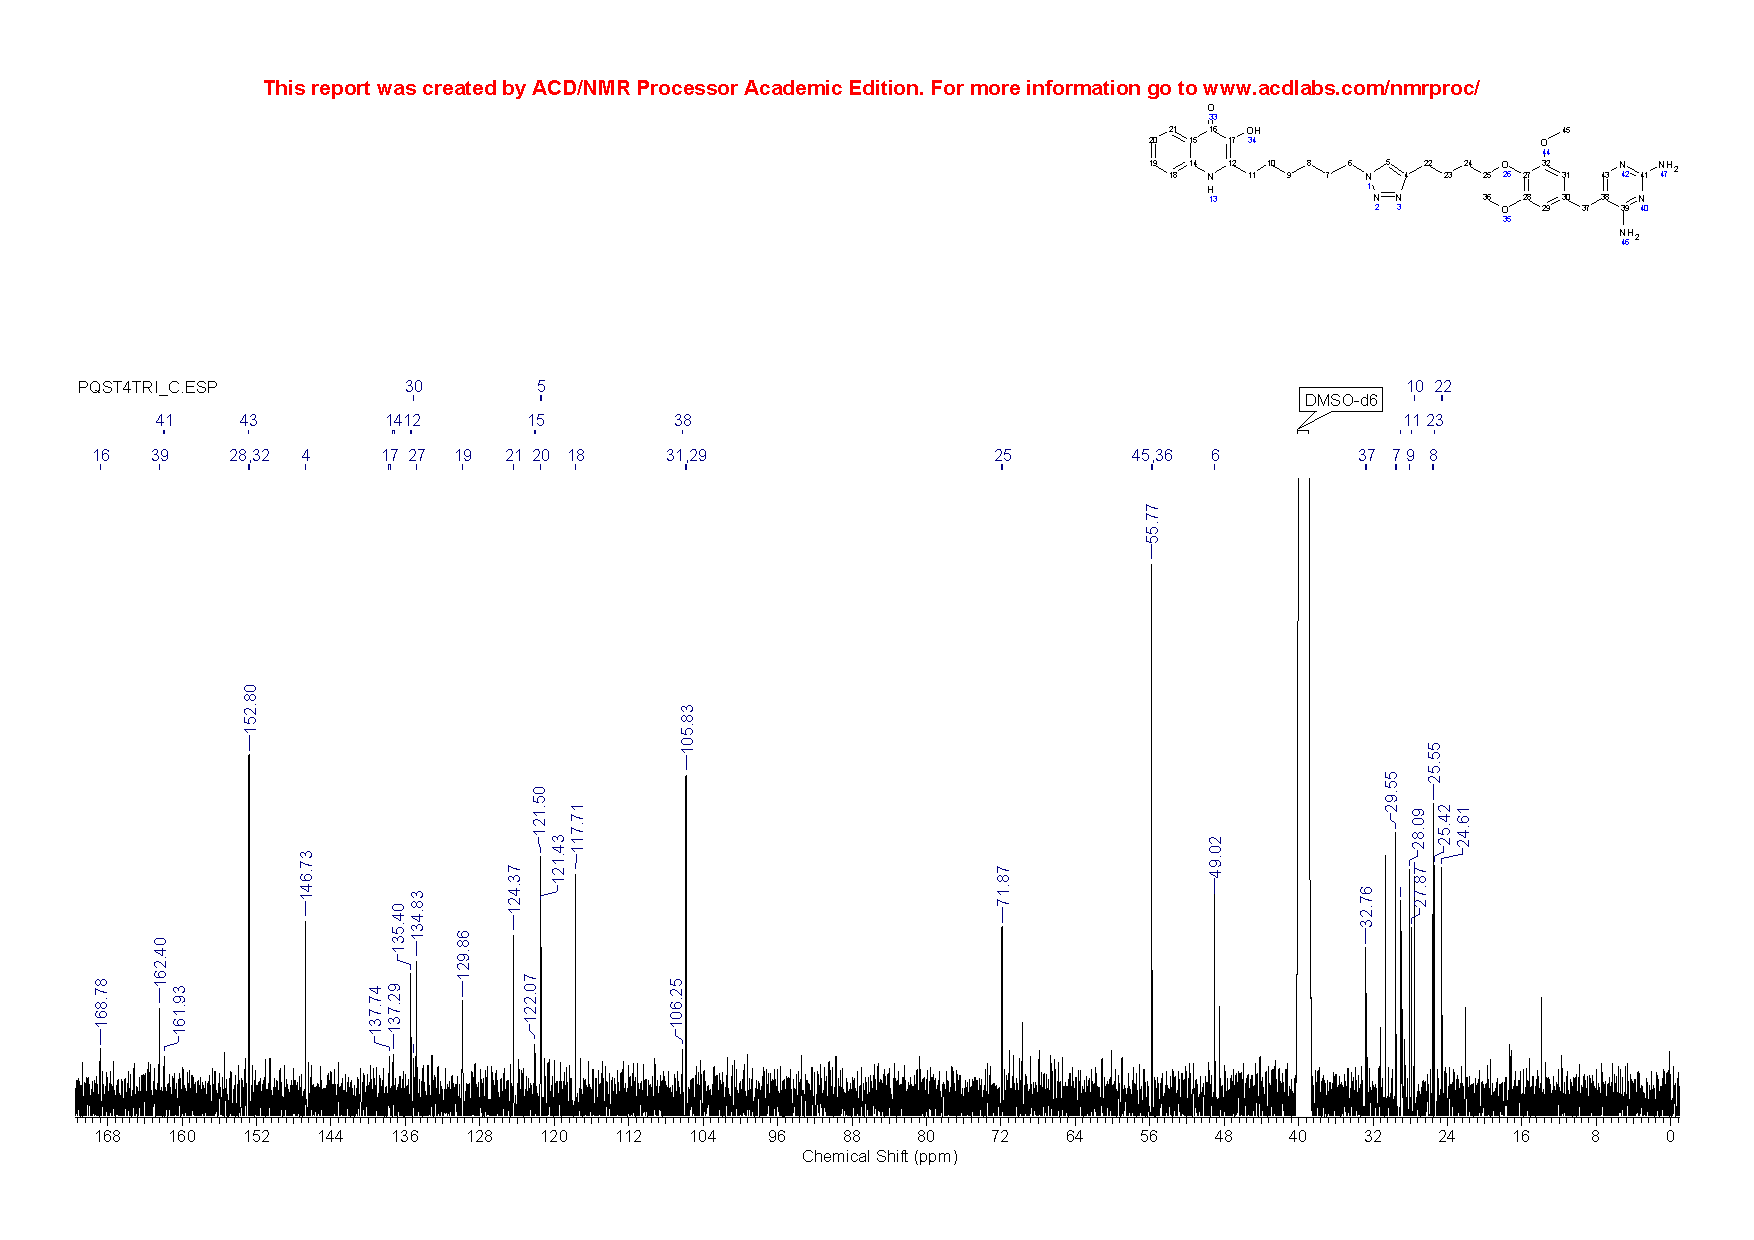
\includegraphics[ width=1.0\textwidth,height=0.43\textheight,keepaspectratio,trim={0 0 0 1.7cm},clip]{PQST4Tri_C.pdf}
\end{figure}

%%%%%%%%%%%%%

\subsection{4\hyp{}Bromo\hyp{}\textit{N}\hyp{}(2\hyp{}oxotetrahydrothiophen\hyp{}3\hyp{}yl)butanamide \compound{cmpd:SHL4Br}}

\begin{figure}[H]
	\centering
		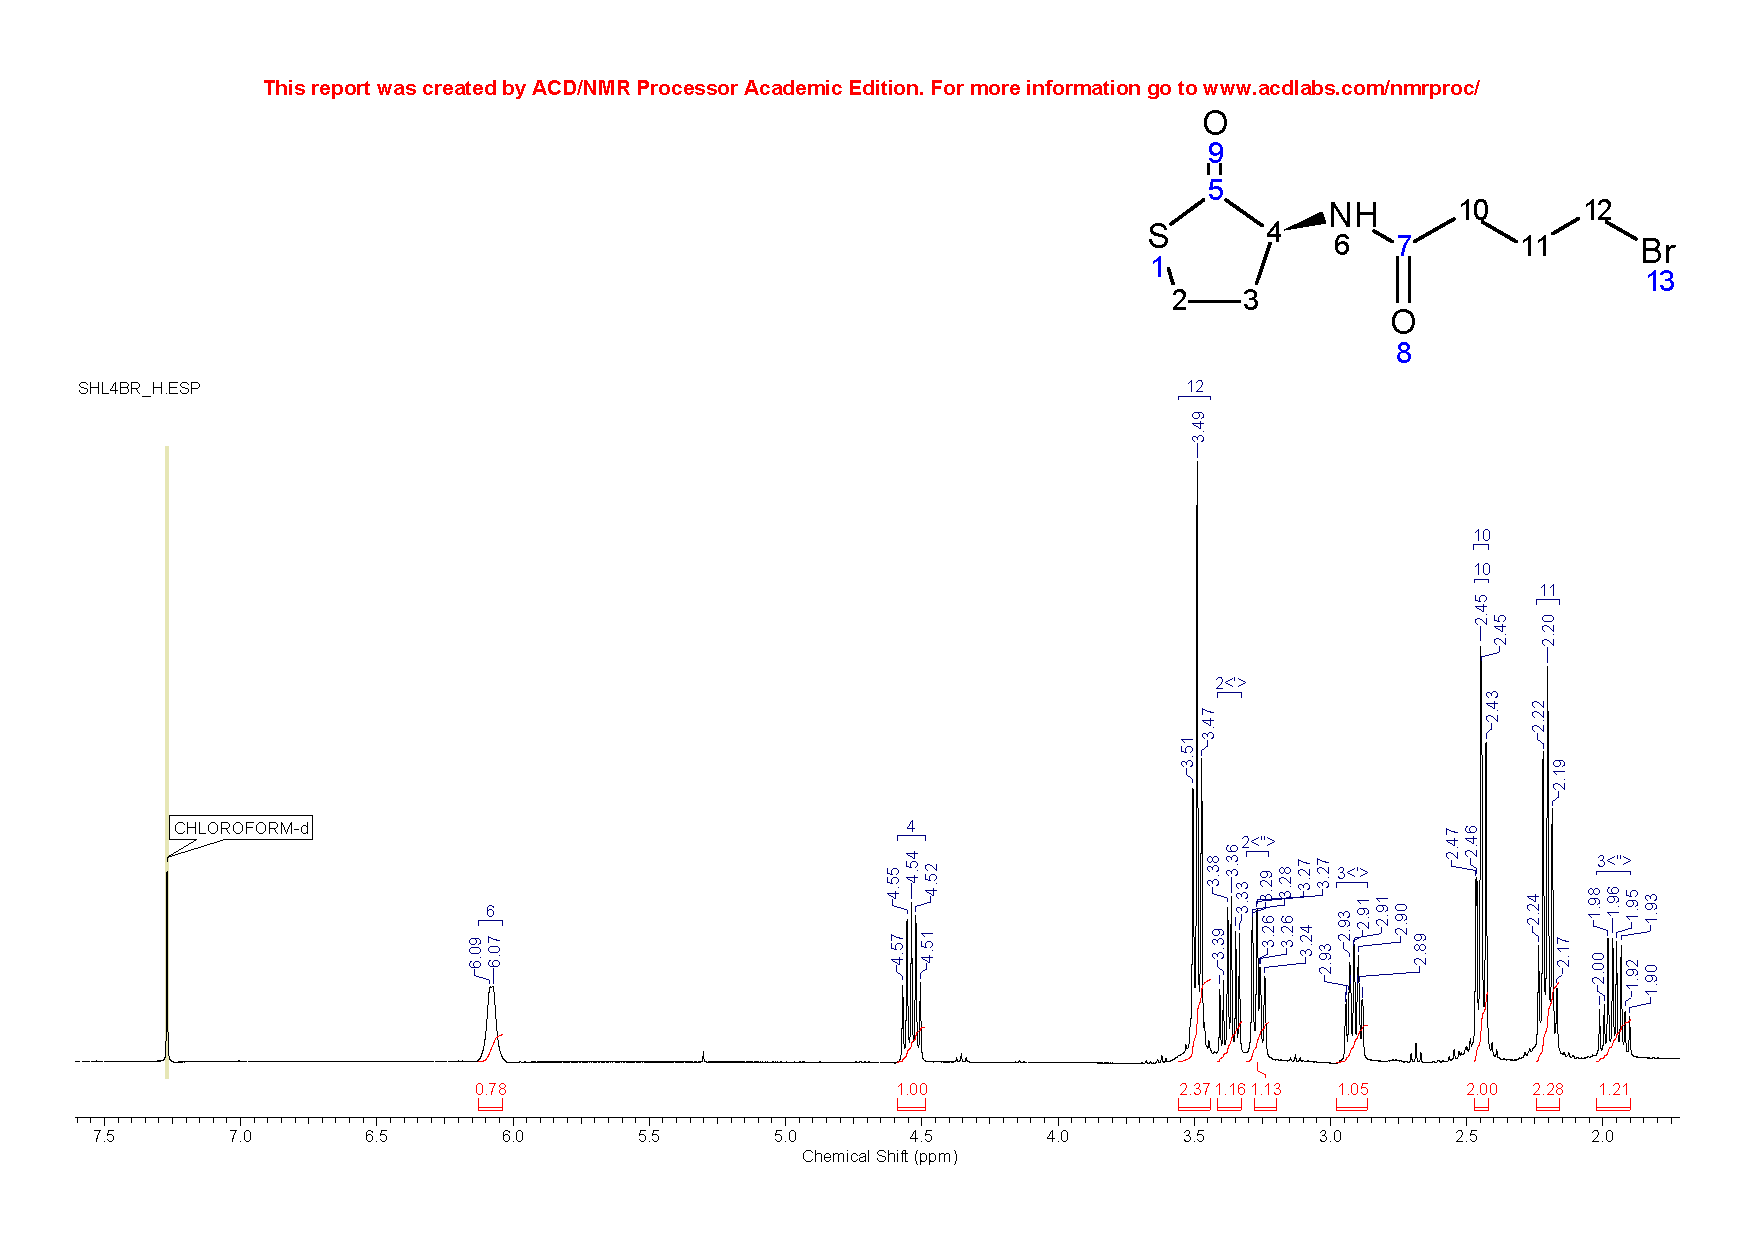
\includegraphics[ width=1.0\textwidth,height=0.43\textheight,keepaspectratio,trim={0 0 0 1.7cm},clip]{SHL4Br_H.pdf}
		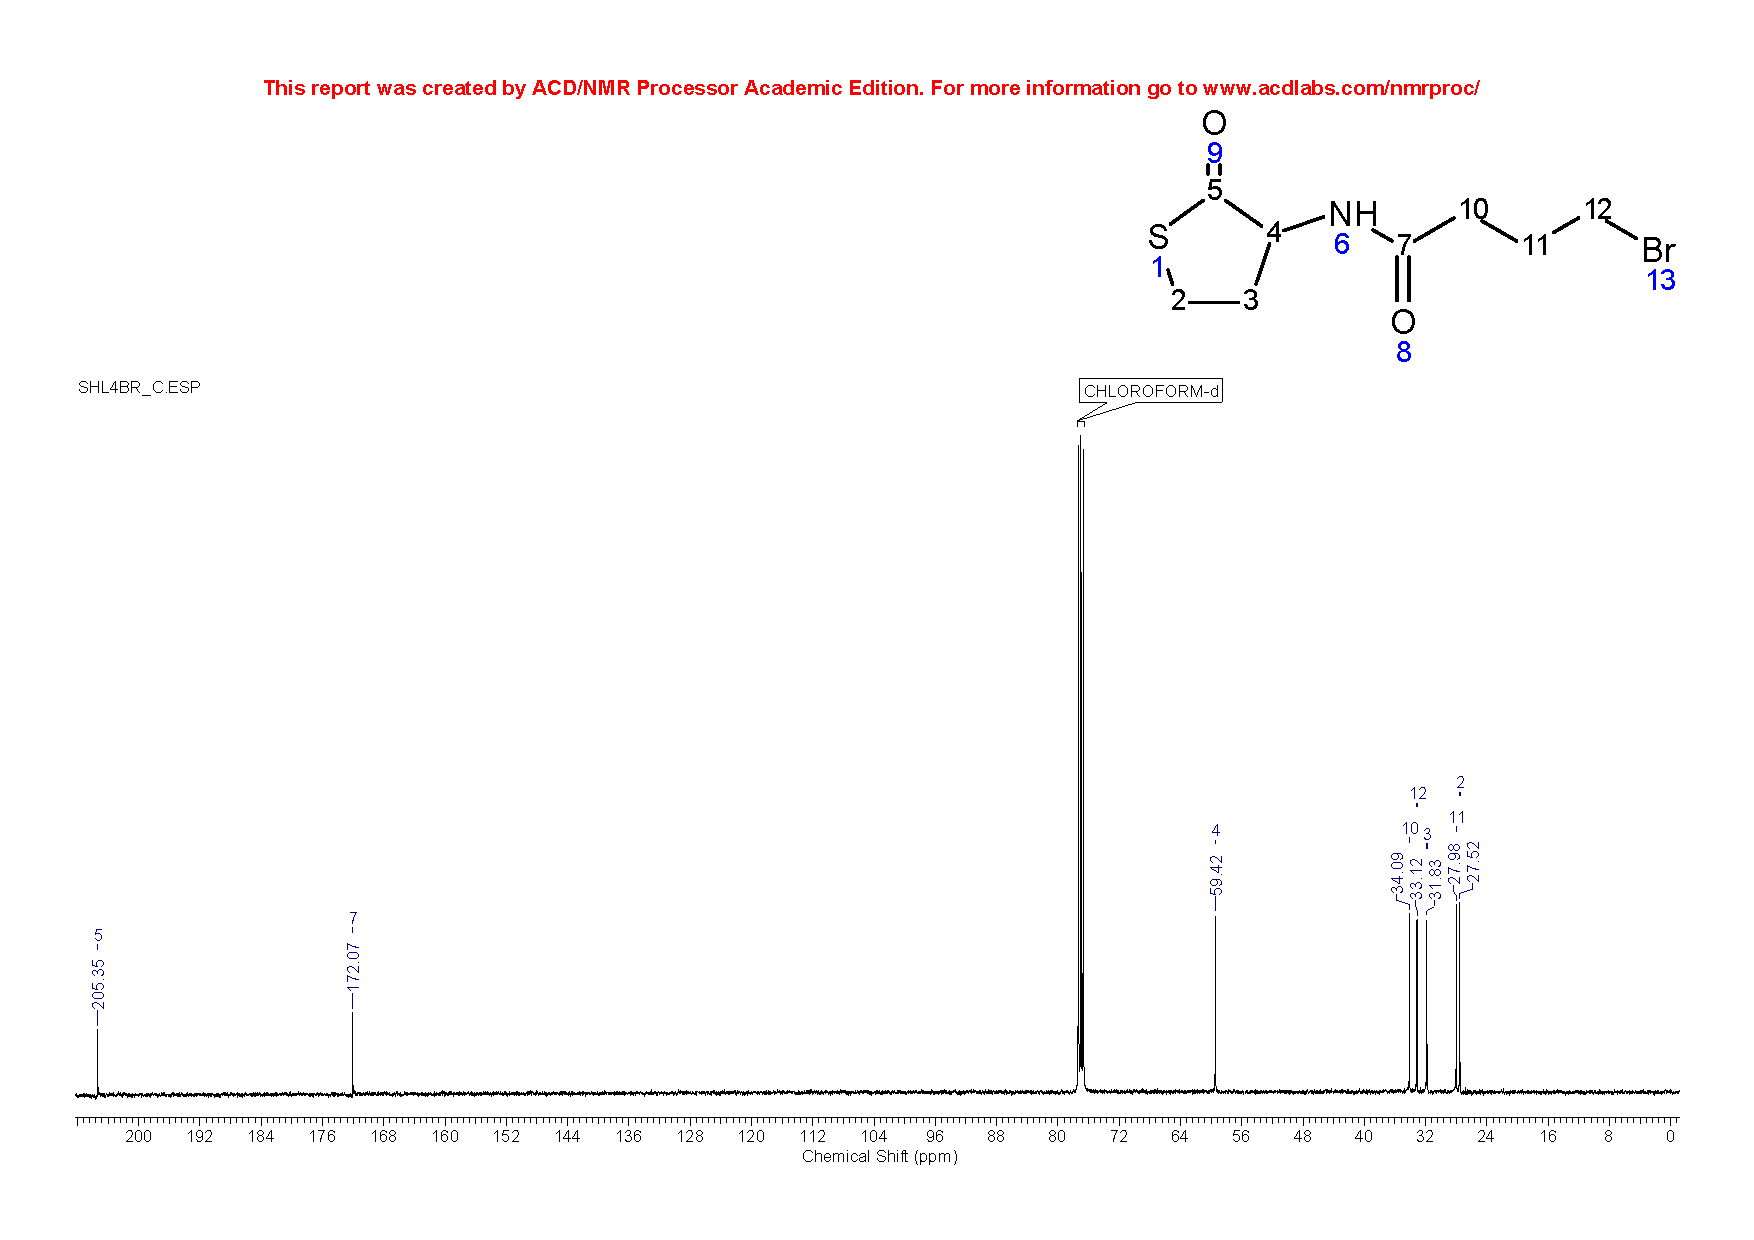
\includegraphics[ width=1.0\textwidth,height=0.43\textheight,keepaspectratio,trim={0 0 0 1.7cm},clip]{SHL4Br_C.pdf}
\end{figure}

\subsection{Methyl 1\hyp{}cyclopropyl\hyp{}6\hyp{}fluoro\hyp{}4\hyp{}oxo\hyp{}7\hyp{}(4\hyp{}(4\hyp{}oxo\hyp{}4\hyp{}((2\hyp{}oxotetrahydrothiophen\hyp{}3\hyp{}yl)amino)butyl)pip\allowbreak erazin\hyp{}1\hyp{}yl)\hyp{}1,4\hyp{}dihydroquinoline\hyp{}3\hyp{}carboxylate \compound{cmpd:SHL4CipMe}}

\begin{figure}[H]
	\centering
		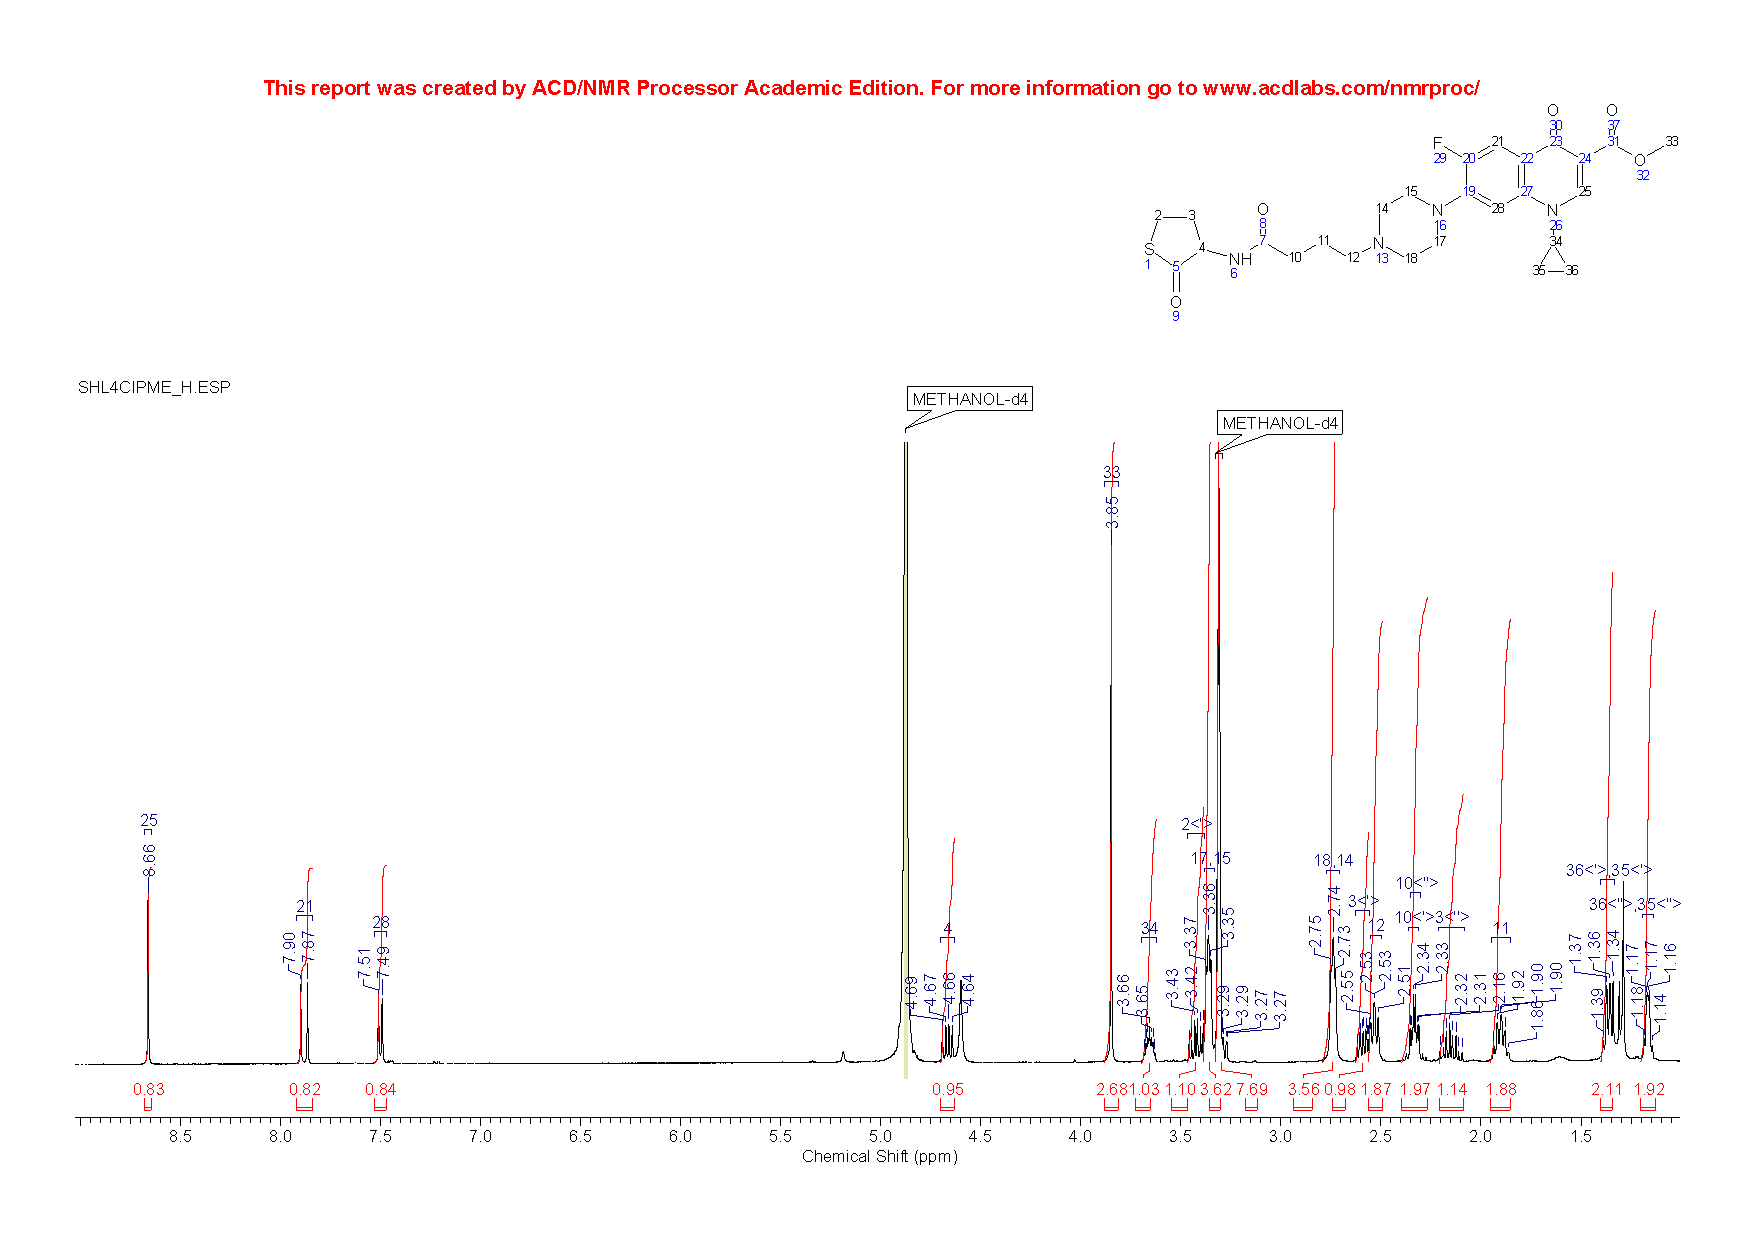
\includegraphics[ width=1.0\textwidth,height=0.43\textheight,keepaspectratio,trim={0 0 0 1.7cm},clip]{SHL4CipMe_H.pdf}
		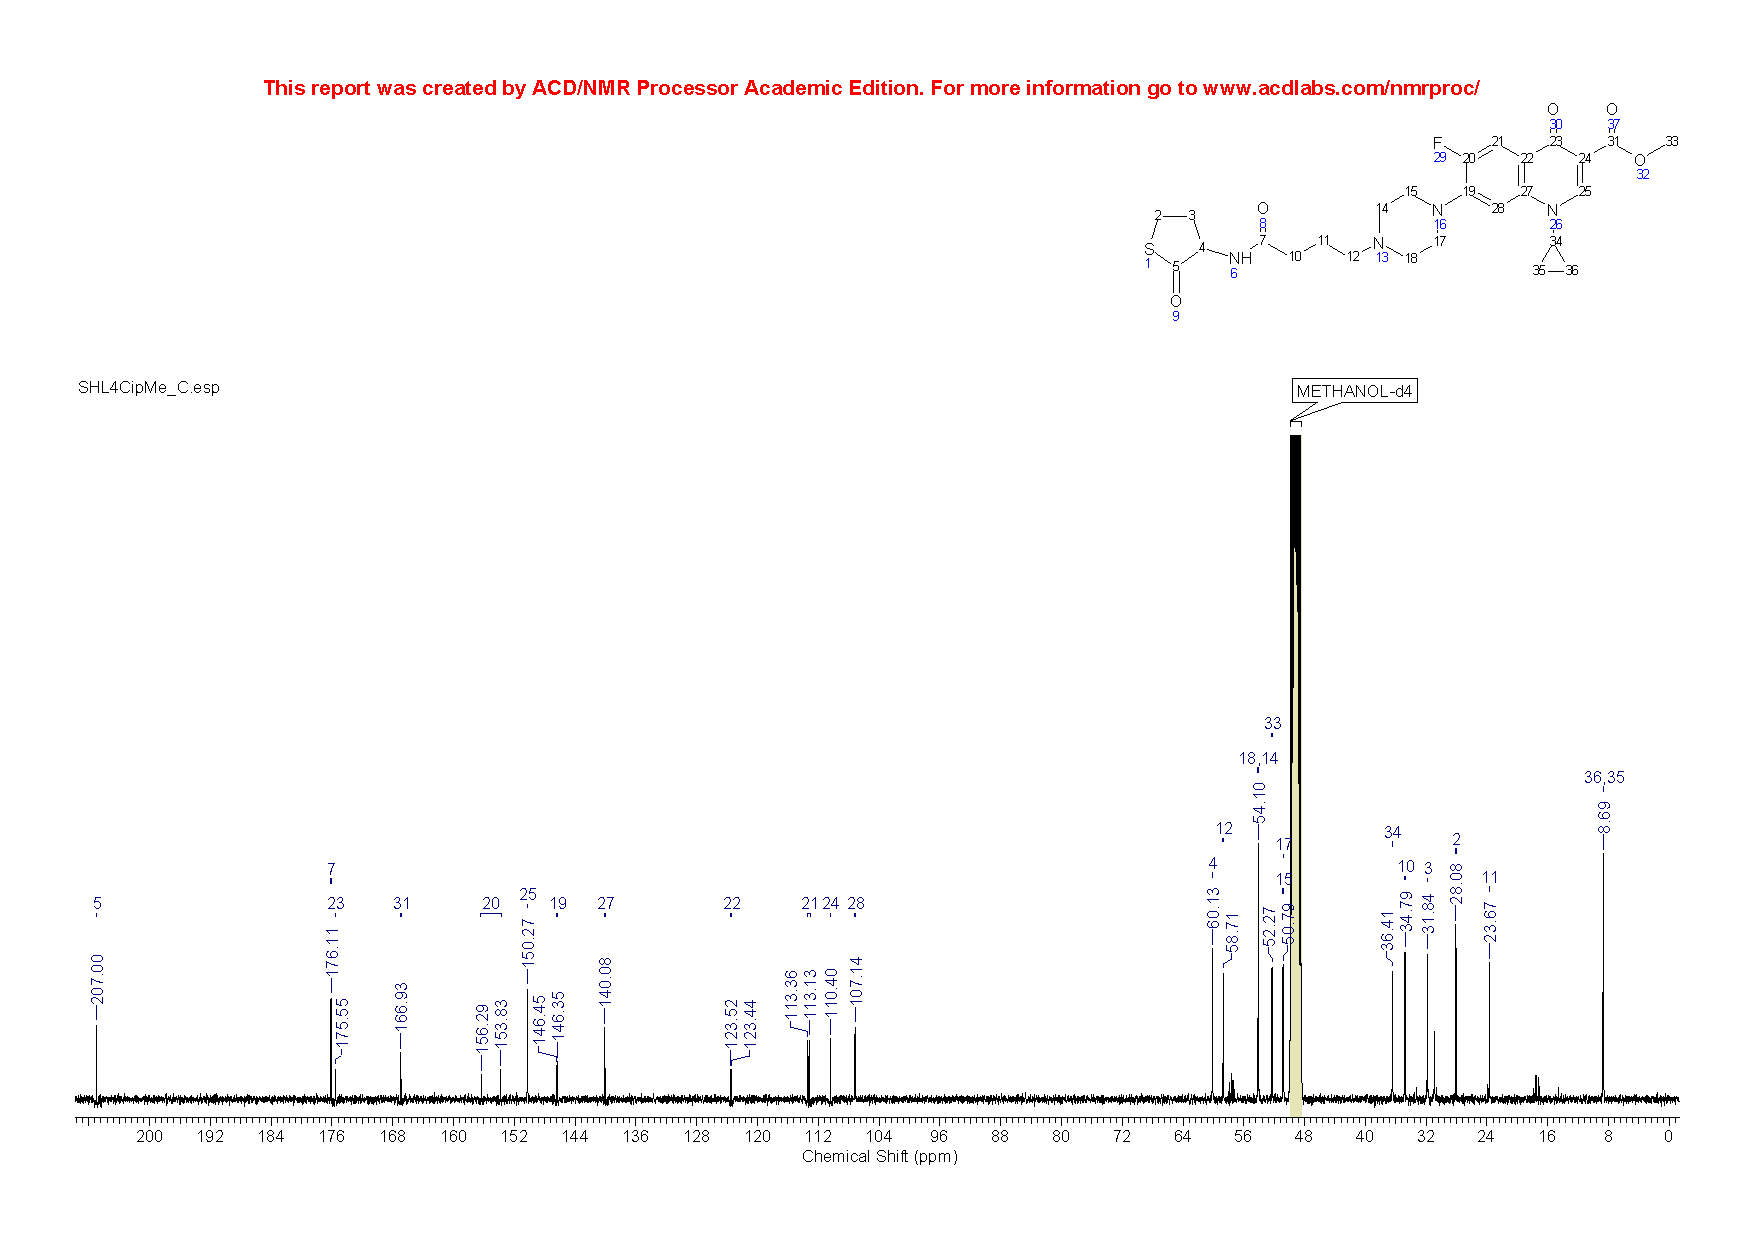
\includegraphics[ width=1.0\textwidth,height=0.43\textheight,keepaspectratio,trim={0 0 0 1.7cm},clip]{SHL4CipMe_C.pdf}
\end{figure}

\subsection{4\hyp{}Azido\hyp{}\textit{N}\hyp{}(2\hyp{}oxotetrahydrothiophen\hyp{}3\hyp{}yl)butanamide \compound{cmpd:SHL4N3}}

\begin{figure}[H]
	\centering
		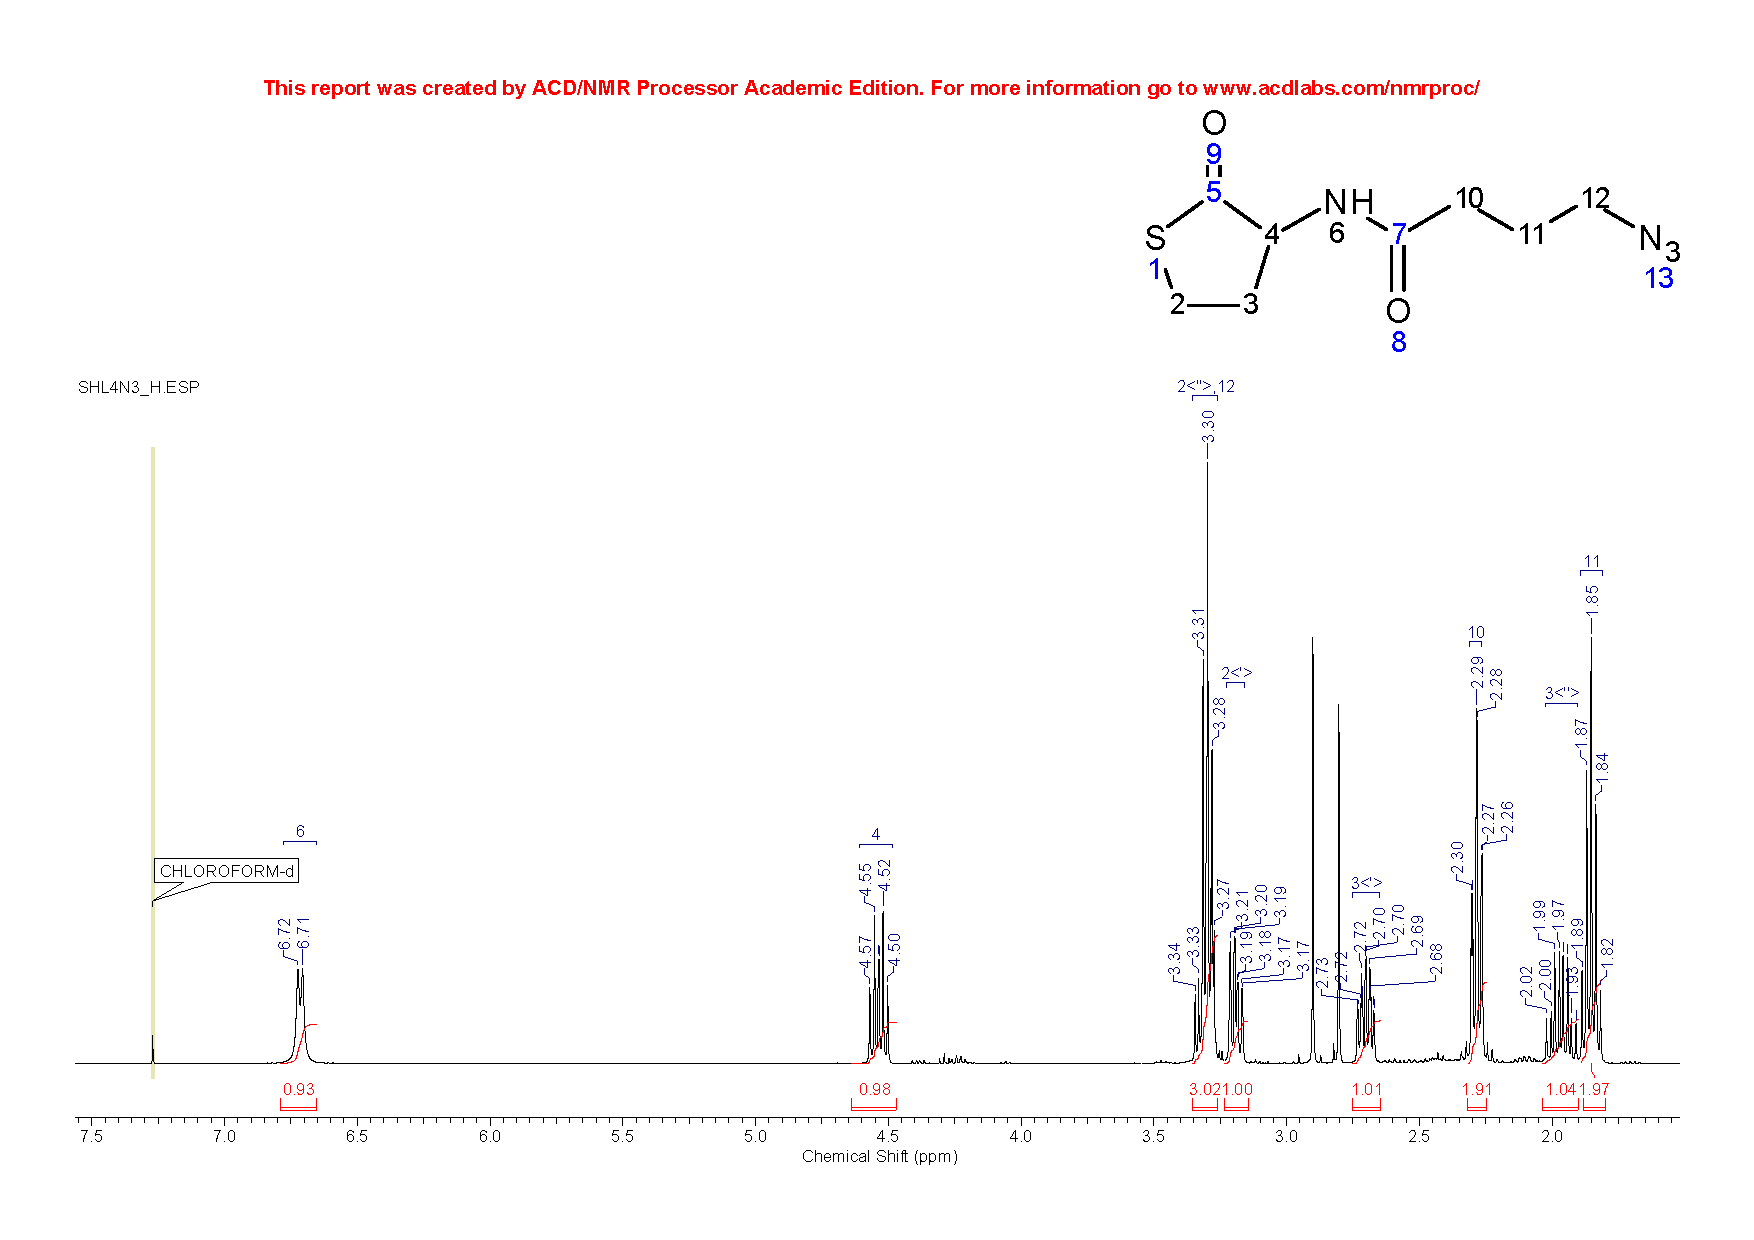
\includegraphics[ width=1.0\textwidth,height=0.43\textheight,keepaspectratio,trim={0 0 0 1.7cm},clip]{SHL4N3_H.pdf}
		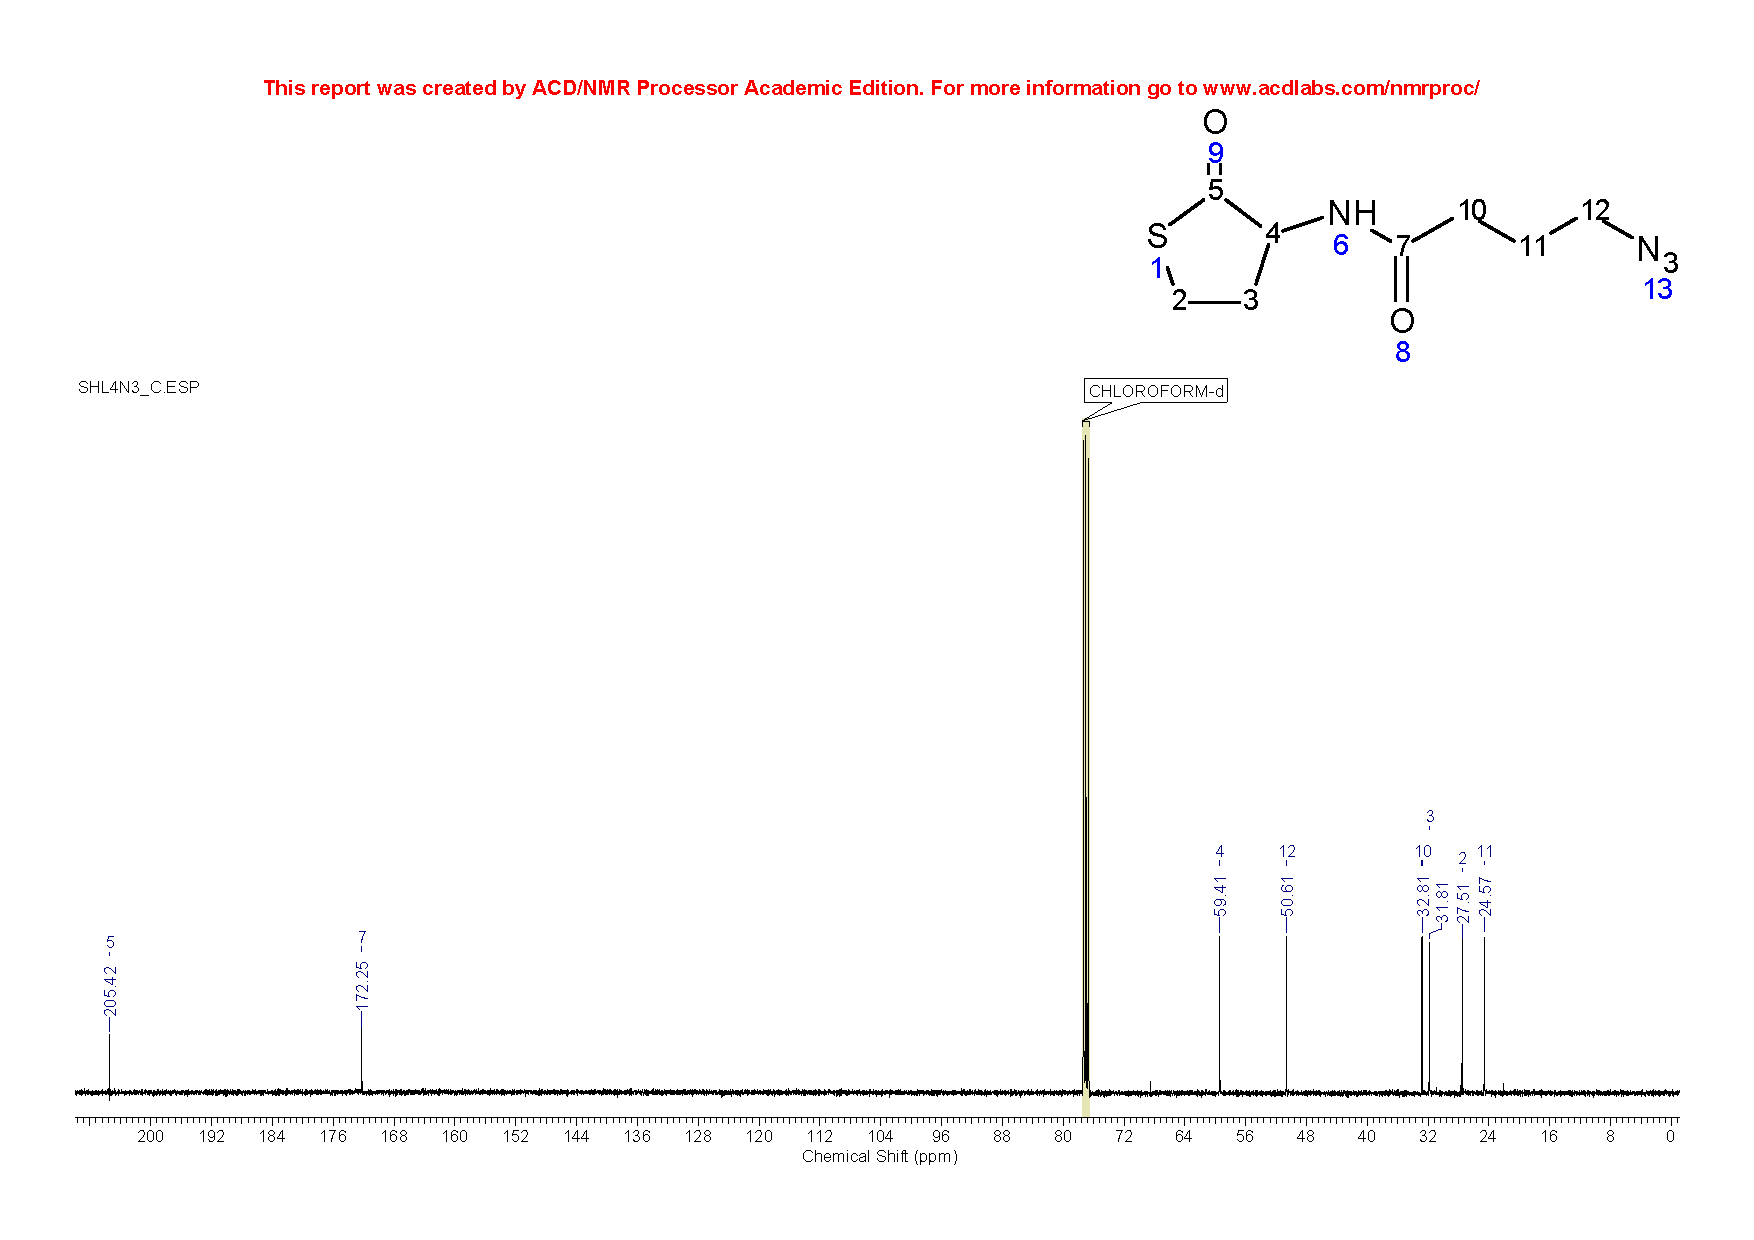
\includegraphics[ width=1.0\textwidth,height=0.43\textheight,keepaspectratio,trim={0 0 0 1.7cm},clip]{SHL4N3_C.pdf}
\end{figure}



\subsection{1\hyp{}Cyclopropyl\hyp{}6\hyp{}fluoro\hyp{}4\hyp{}oxo\hyp{}7\hyp{}(4\hyp{}(4\hyp{}(1\hyp{}(4\hyp{}oxo\hyp{}4\hyp{}((2\hyp{}oxotetrahydrothiophen\hyp{}3\hyp{}yl)amino)butyl)\hyp{}1\textit{H}\hyp{}1,2,3\hyp{}triazol\hyp{}4\hyp{}yl)butyl)piperazin\hyp{}1\hyp{}yl)\hyp{}1,4\hyp{}dihydroquin\allowbreak ol\hyp{}ine\hyp{}3\hyp{}carboxylic acid \compound{cmpd:SHL4T4Cip}}

\begin{figure}[H]
	\centering
		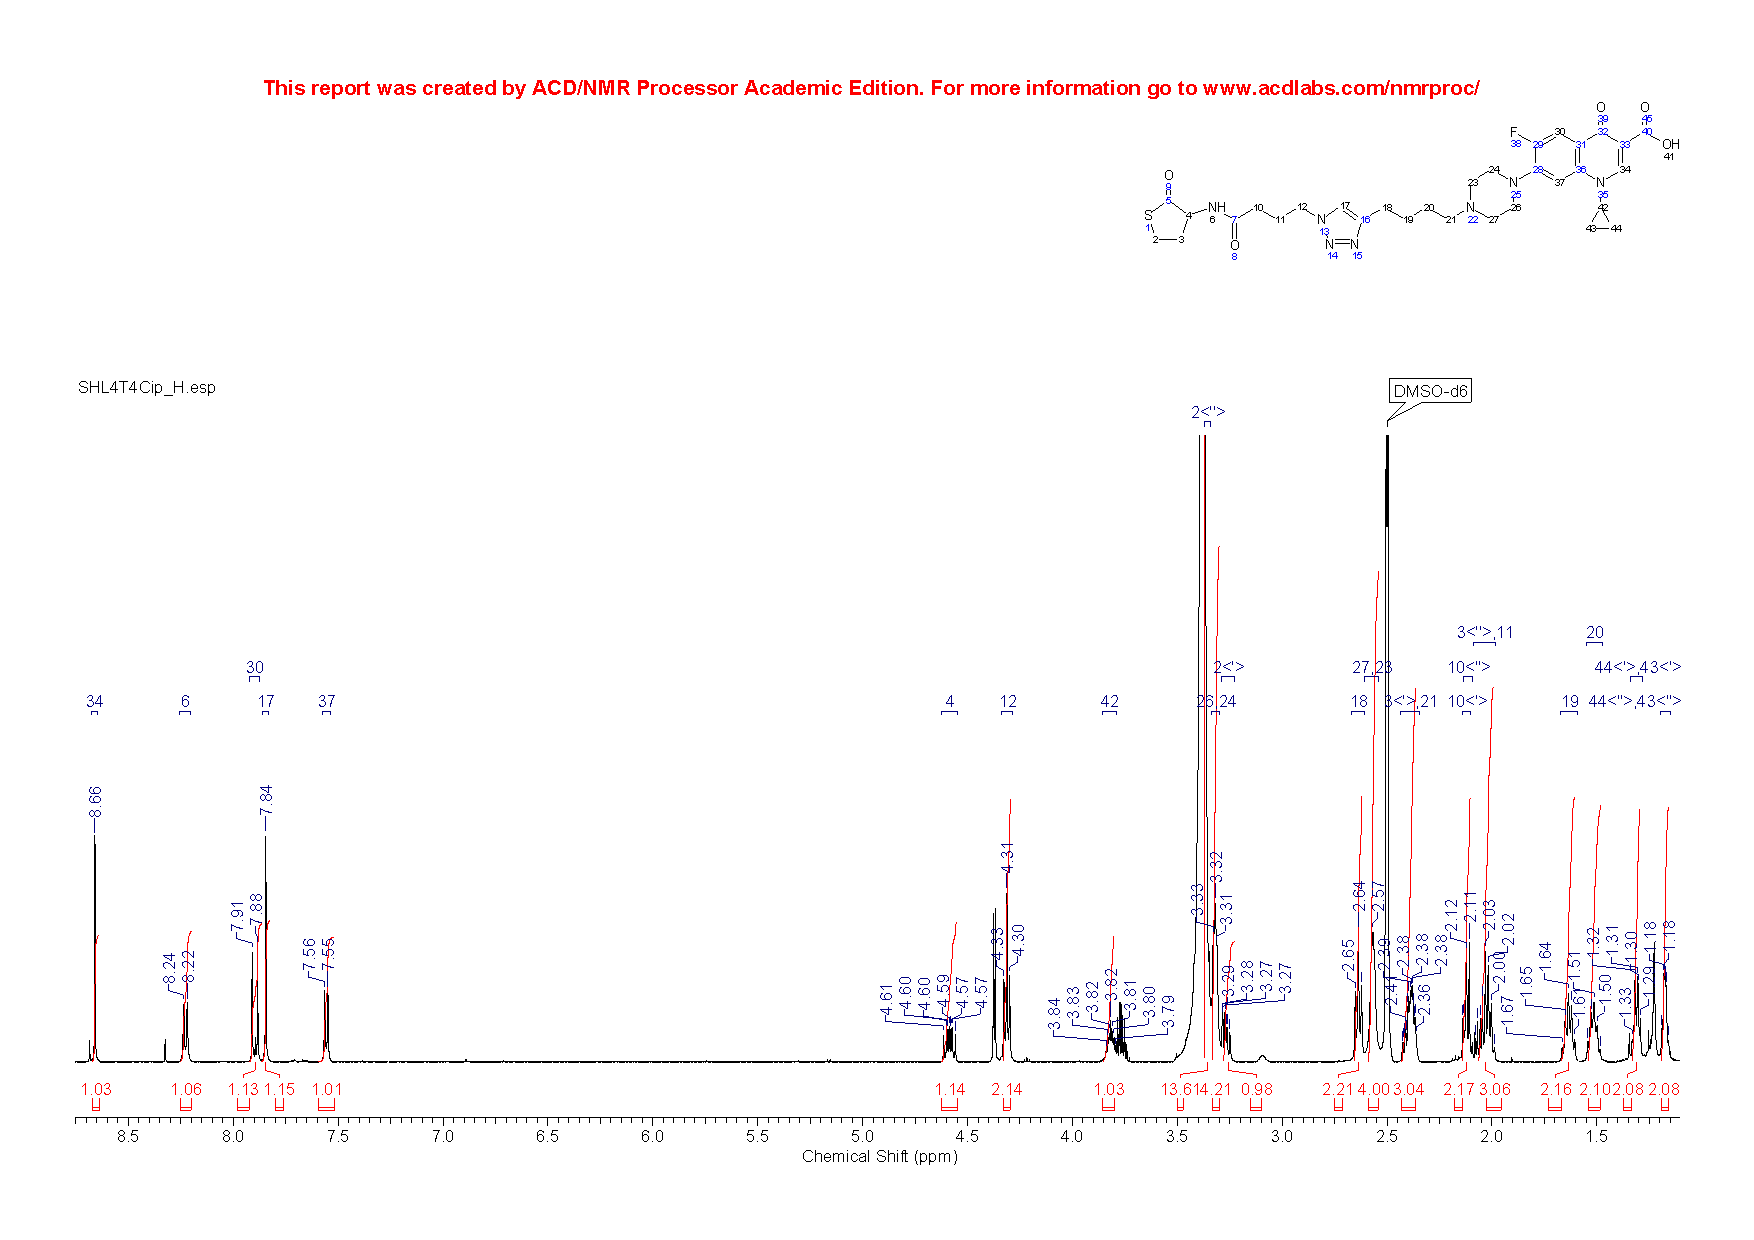
\includegraphics[ width=1.0\textwidth,height=0.43\textheight,keepaspectratio,trim={0 0 0 1.7cm},clip]{SHL4T4Cip_H.pdf}
		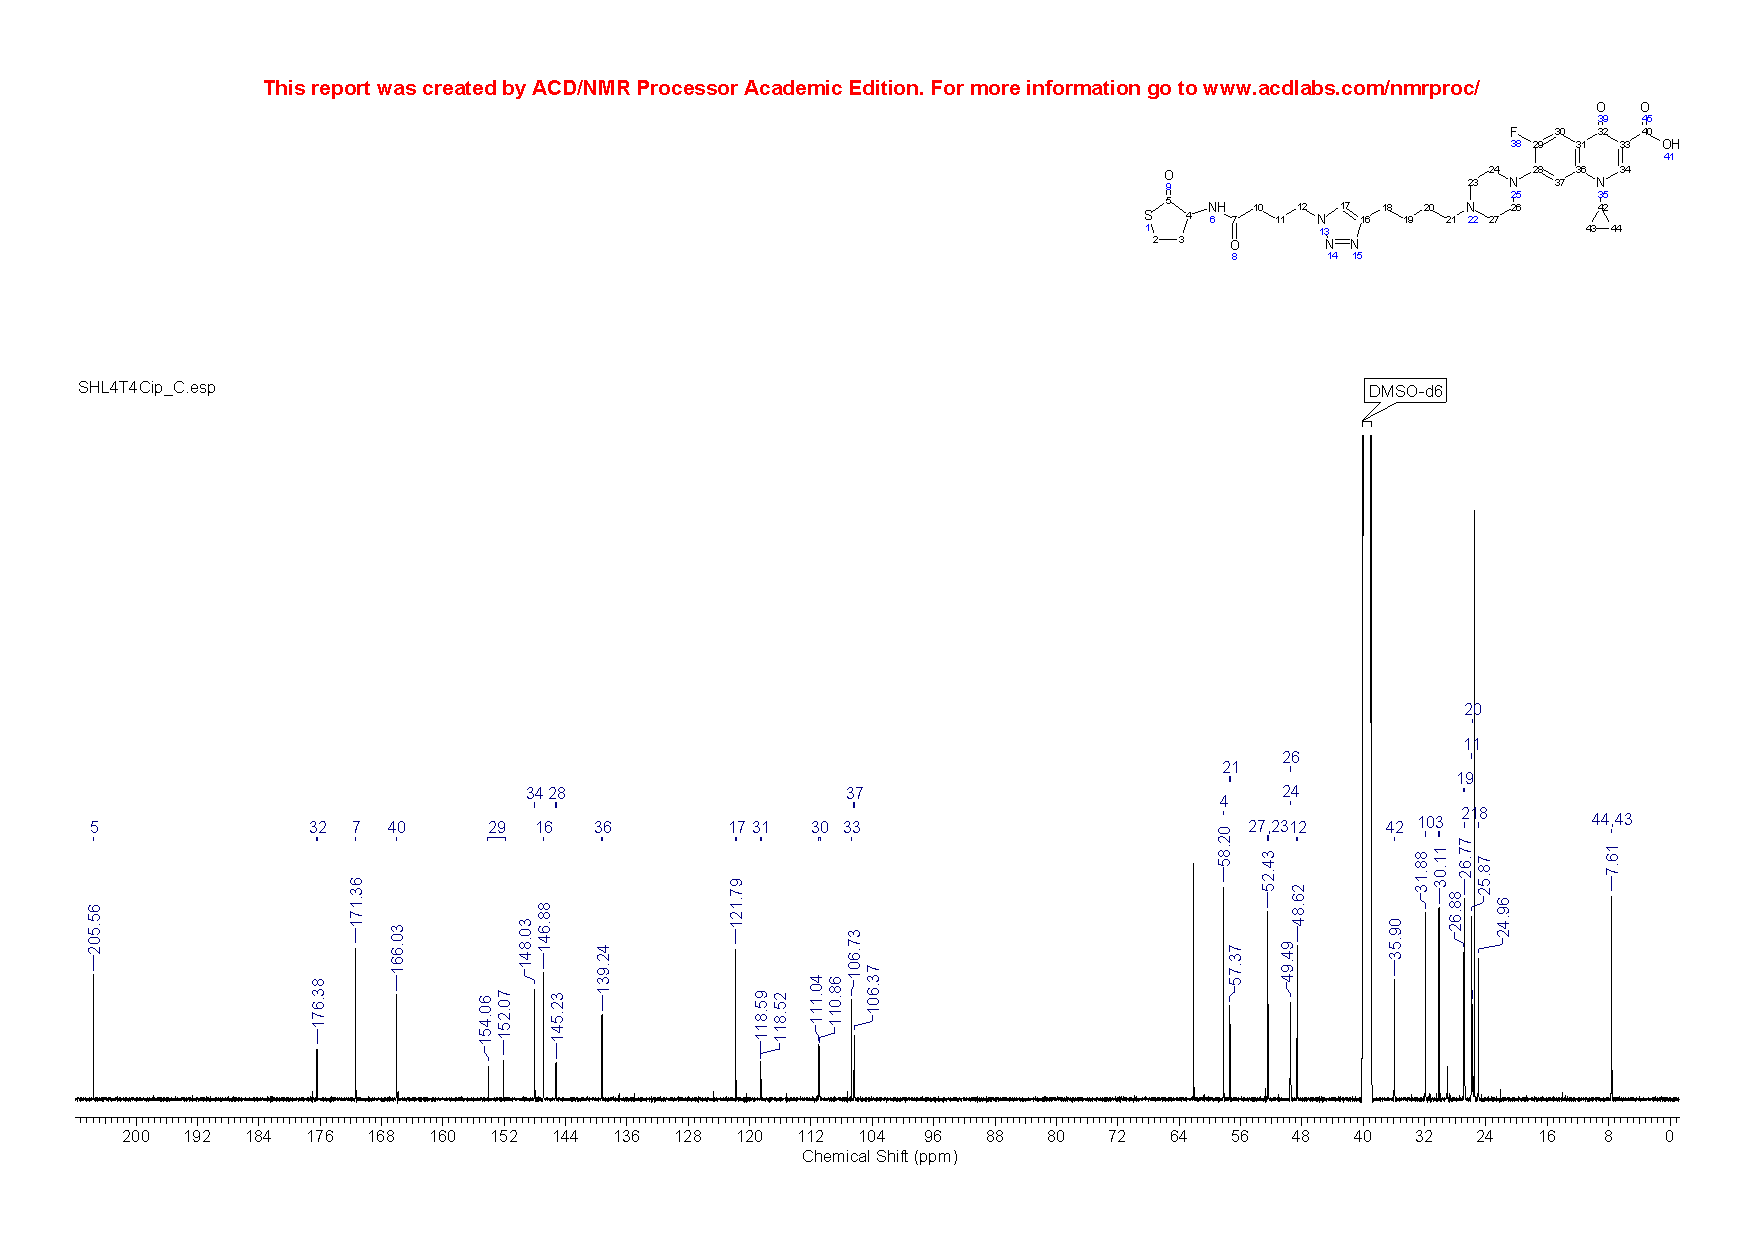
\includegraphics[ width=1.0\textwidth,height=0.43\textheight,keepaspectratio,trim={0 0 0 1.7cm},clip]{SHL4T4Cip_C.pdf}
\end{figure}

\subsection{1\hyp{}Cyclopropyl\hyp{}6\hyp{}fluoro\hyp{}4\hyp{}oxo\hyp{}7\hyp{}(4\hyp{}((((4\hyp{}(1\hyp{}(4\hyp{}oxo\hyp{}4\hyp{}((2\hyp{}oxotetrahydrothiophen\allowbreak \hyp{}3\hyp{}yl)amino)butyl)\hyp{}1\textit{H}\hyp{}1,2,3\hyp{}triazol\hyp{}4\hyp{}yl)butanoyl)oxy)methoxy)carbonyl)pip\allowbreak er\hyp{}azin\hyp{}1\hyp{}yl)\hyp{}1,4\hyp{}dihydroquinoline\hyp{}3\hyp{}carboxylic acid \compound{cmpd:SHL4THCip}}

\begin{figure}[H]
	\centering
		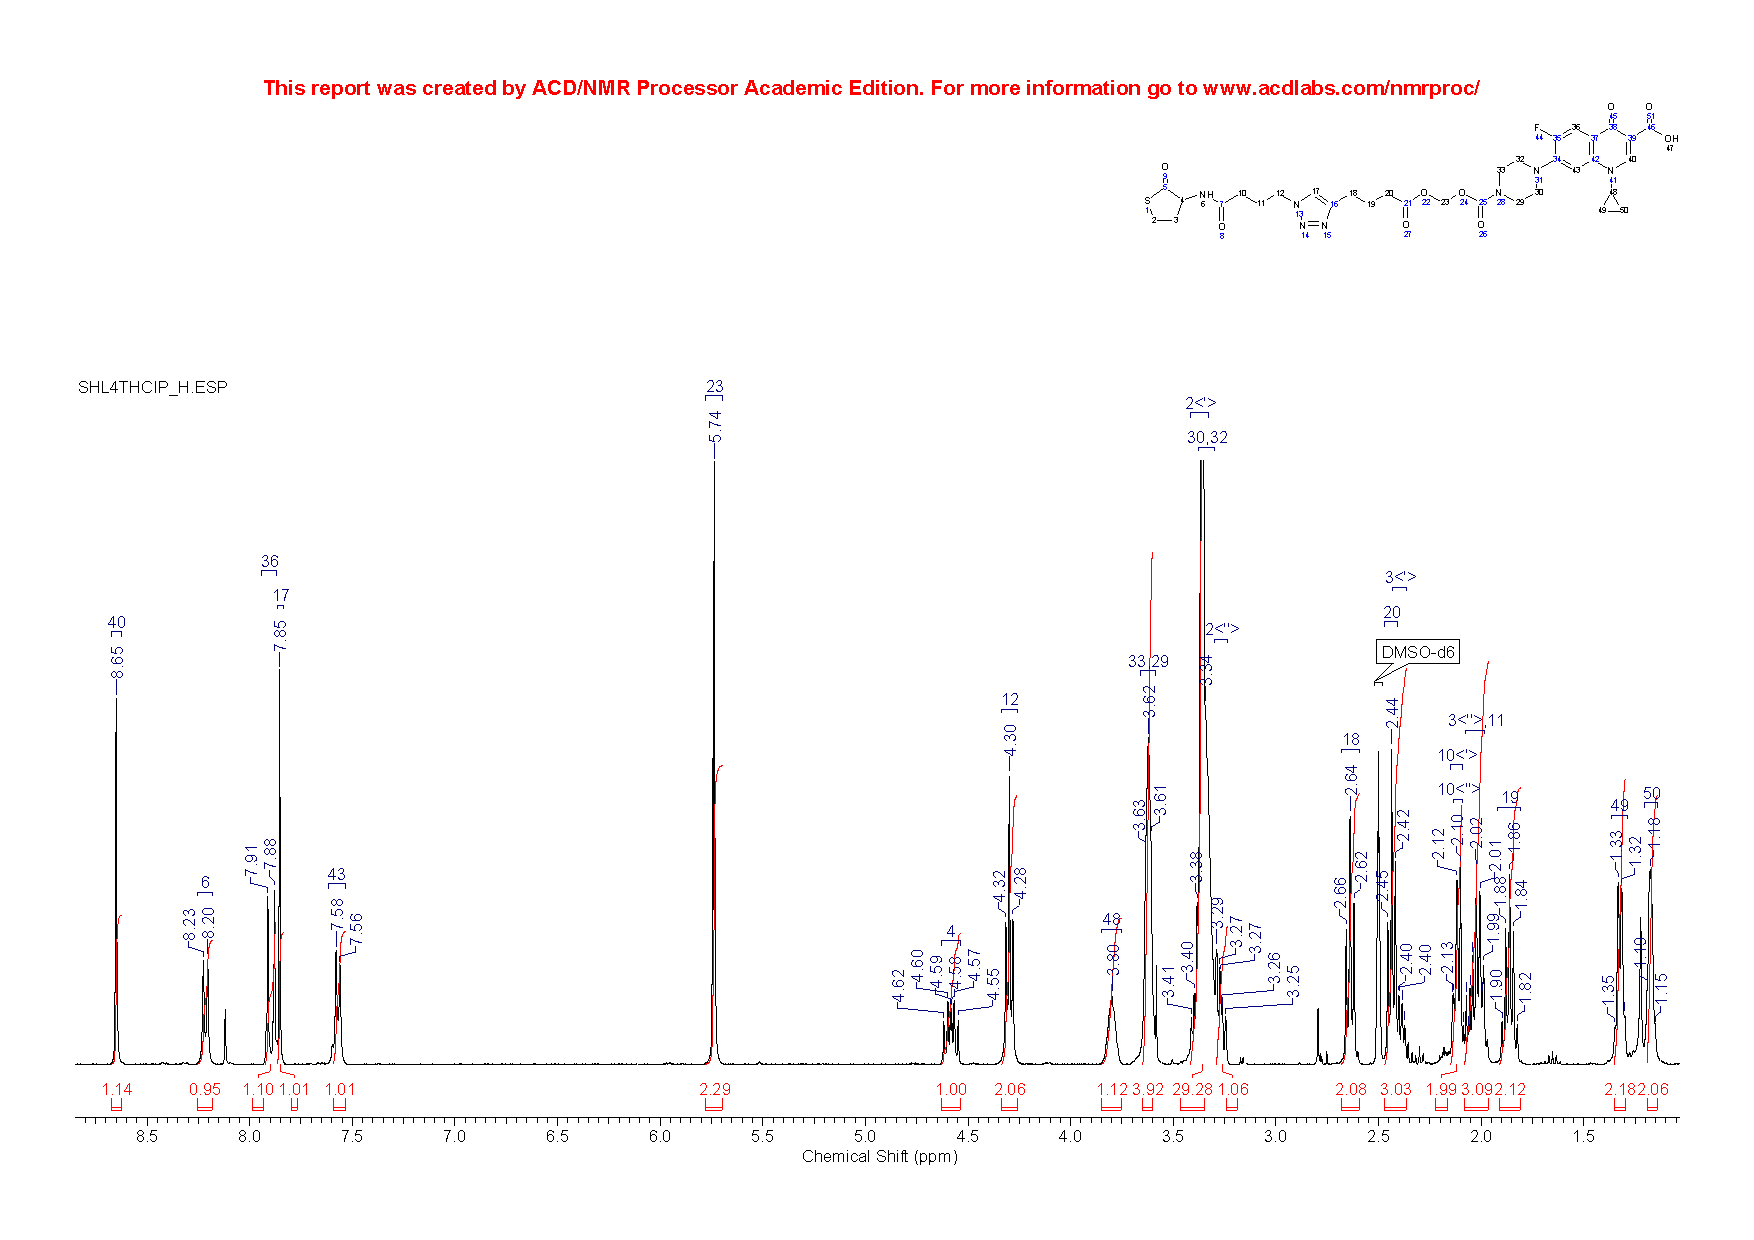
\includegraphics[ width=1.0\textwidth,height=0.43\textheight,keepaspectratio,trim={0 0 0 1.7cm},clip]{SHL4THCip_H.pdf}
		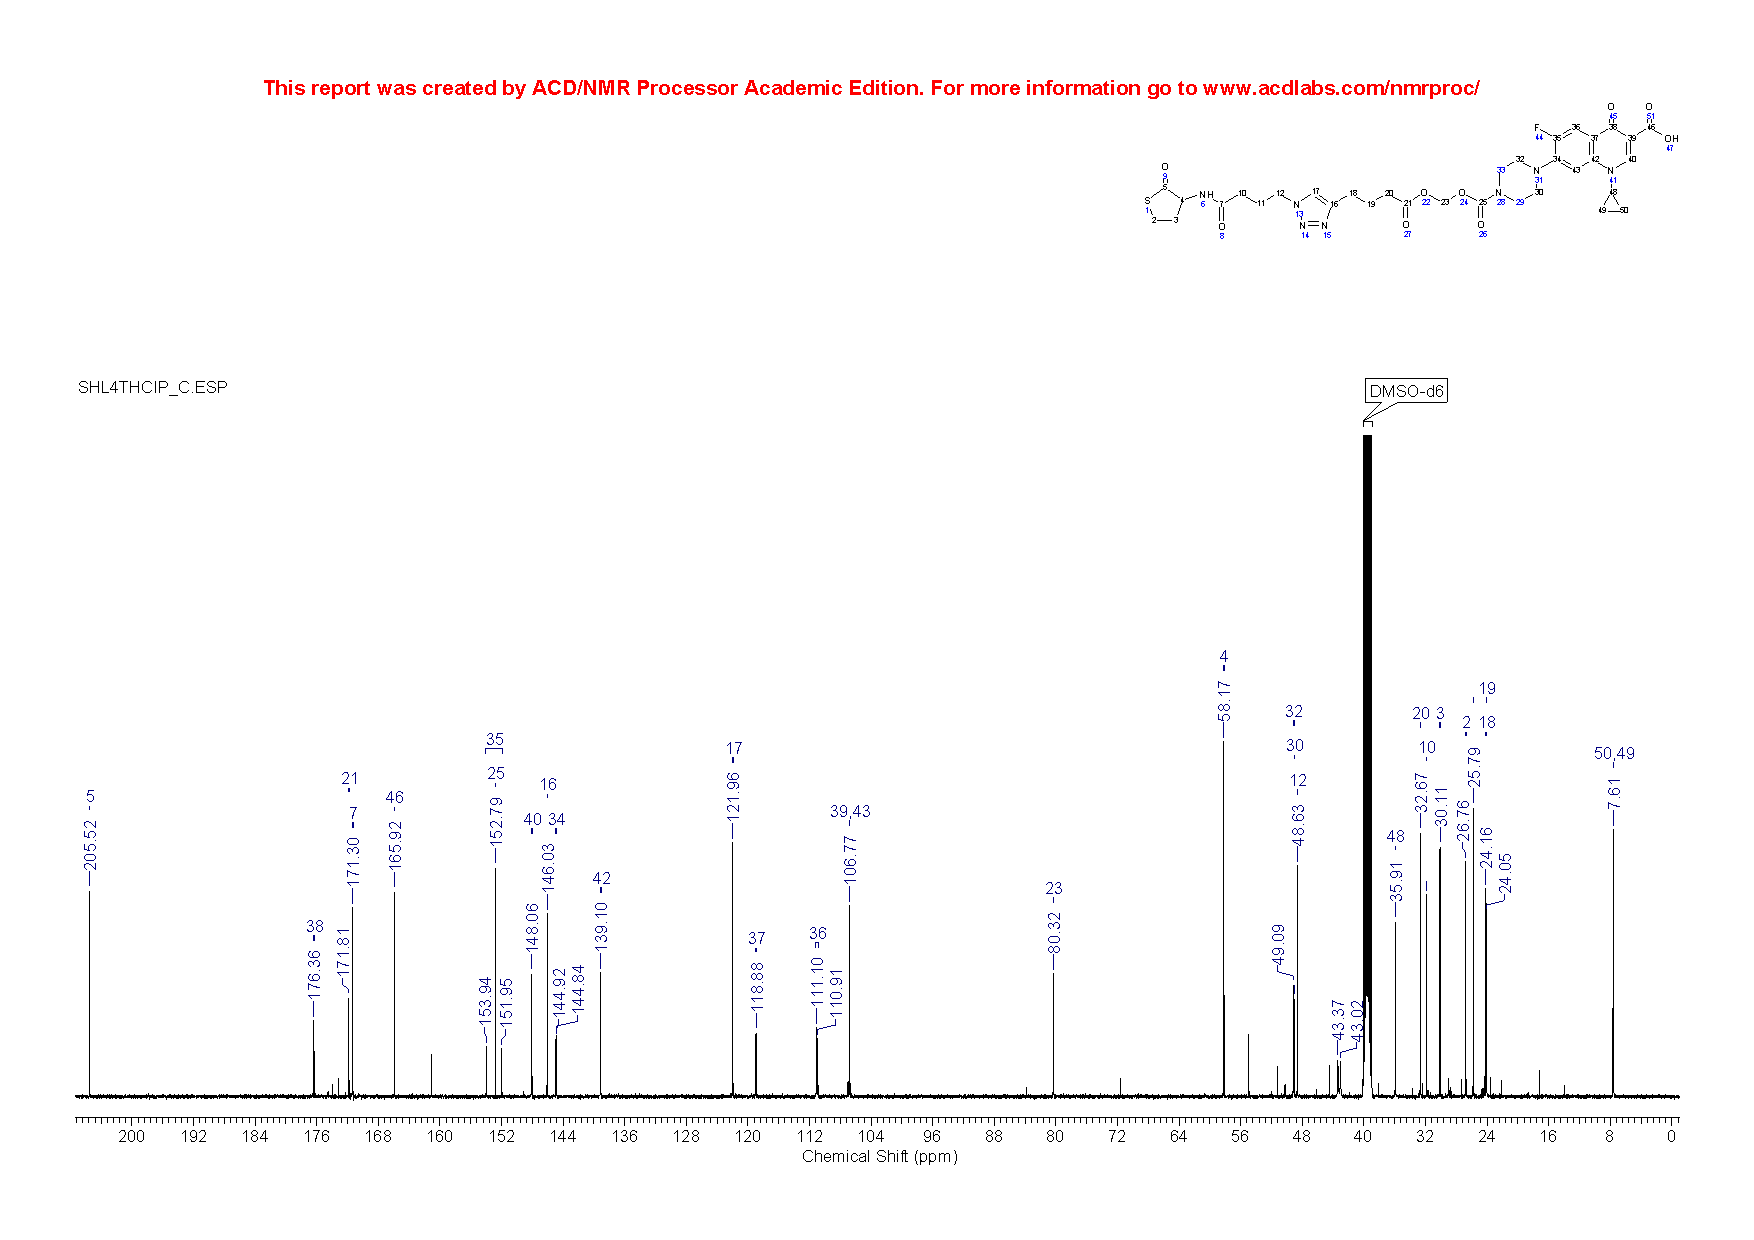
\includegraphics[ width=1.0\textwidth,height=0.43\textheight,keepaspectratio,trim={0 0 0 1.7cm},clip]{SHL4THCip_C.pdf}
\end{figure}

\subsection{4\hyp{}Bromo\hyp{}\textit{N}\hyp{}(2\hyp{}methoxyphenyl)butanamide \compound{cmpd:2MeOA4Br}}

\begin{figure}[H]
	\centering
		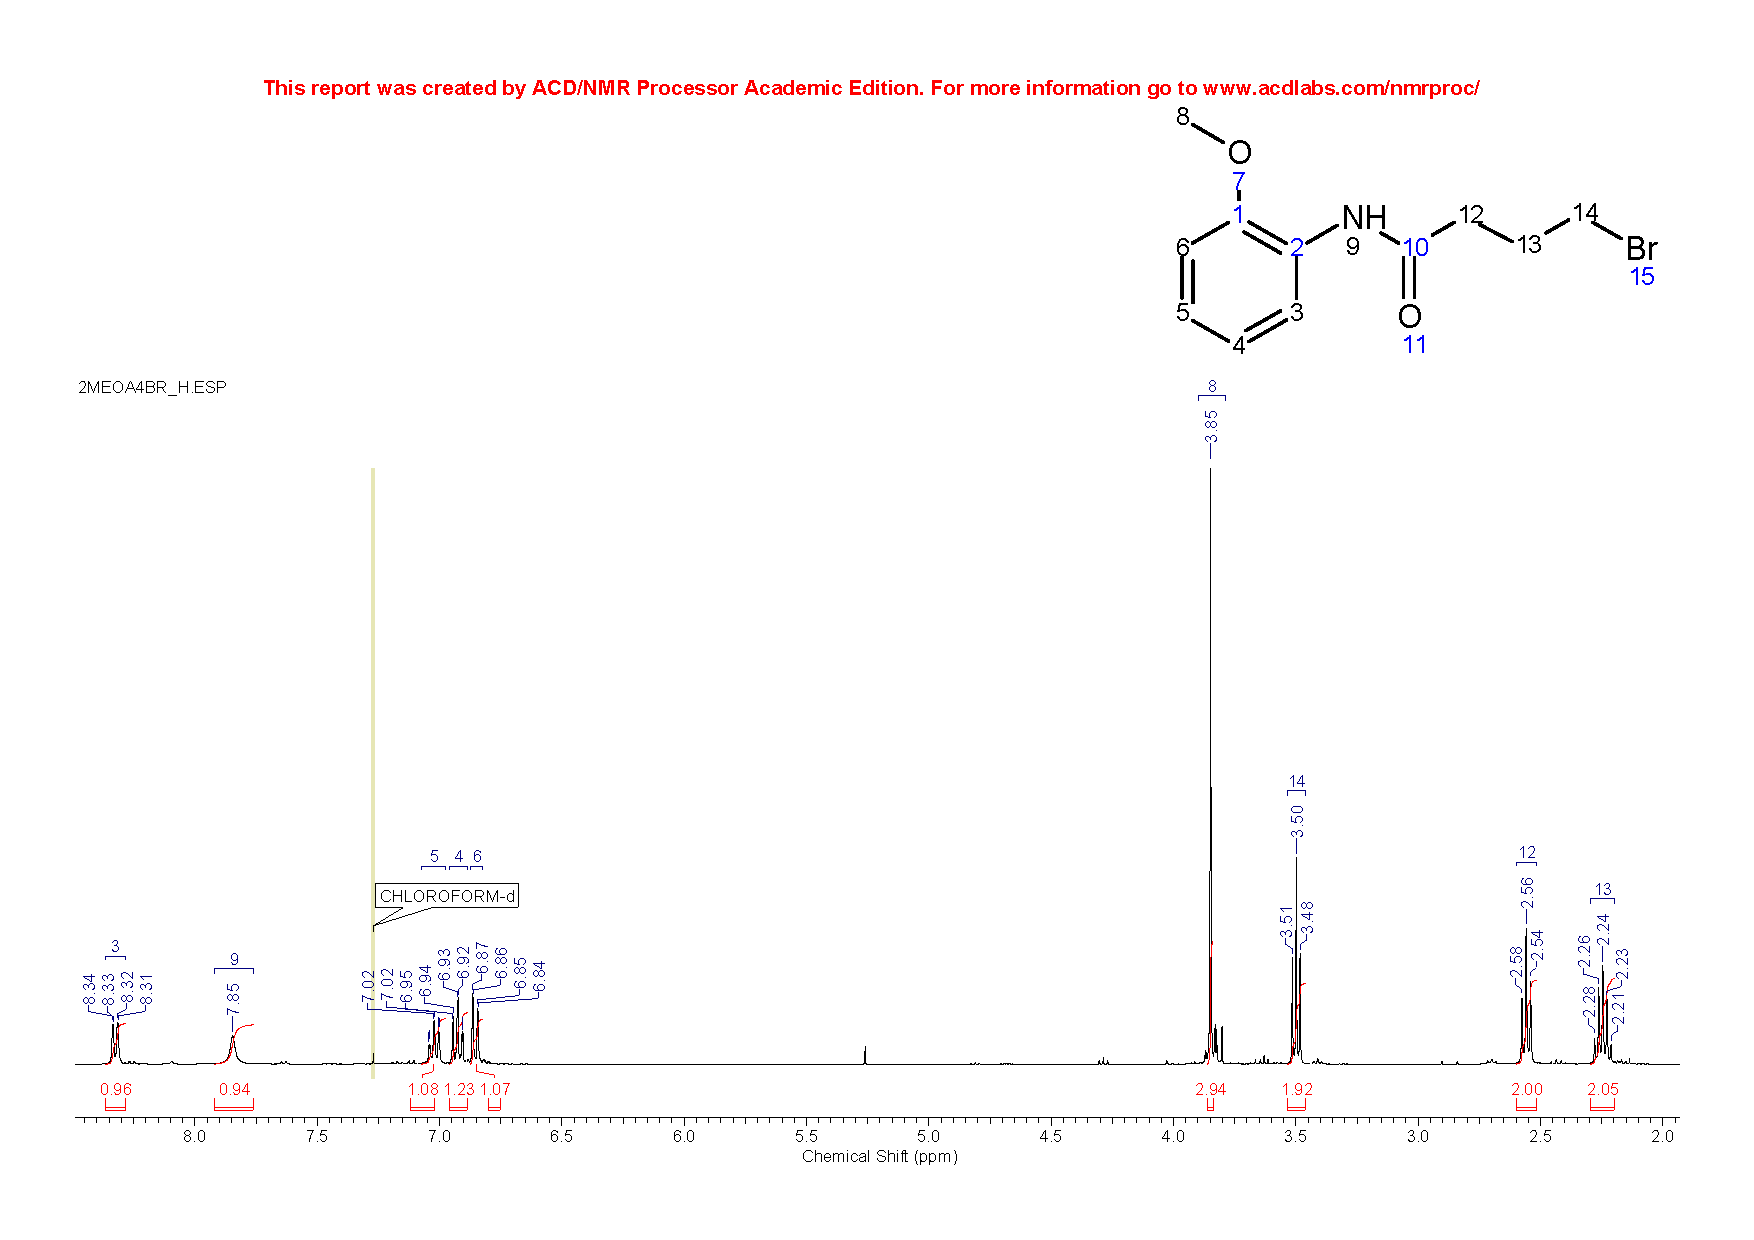
\includegraphics[ width=1.0\textwidth,height=0.43\textheight,keepaspectratio,trim={0 0 0 1.7cm},clip]{2MeOA4Br_H.pdf}
		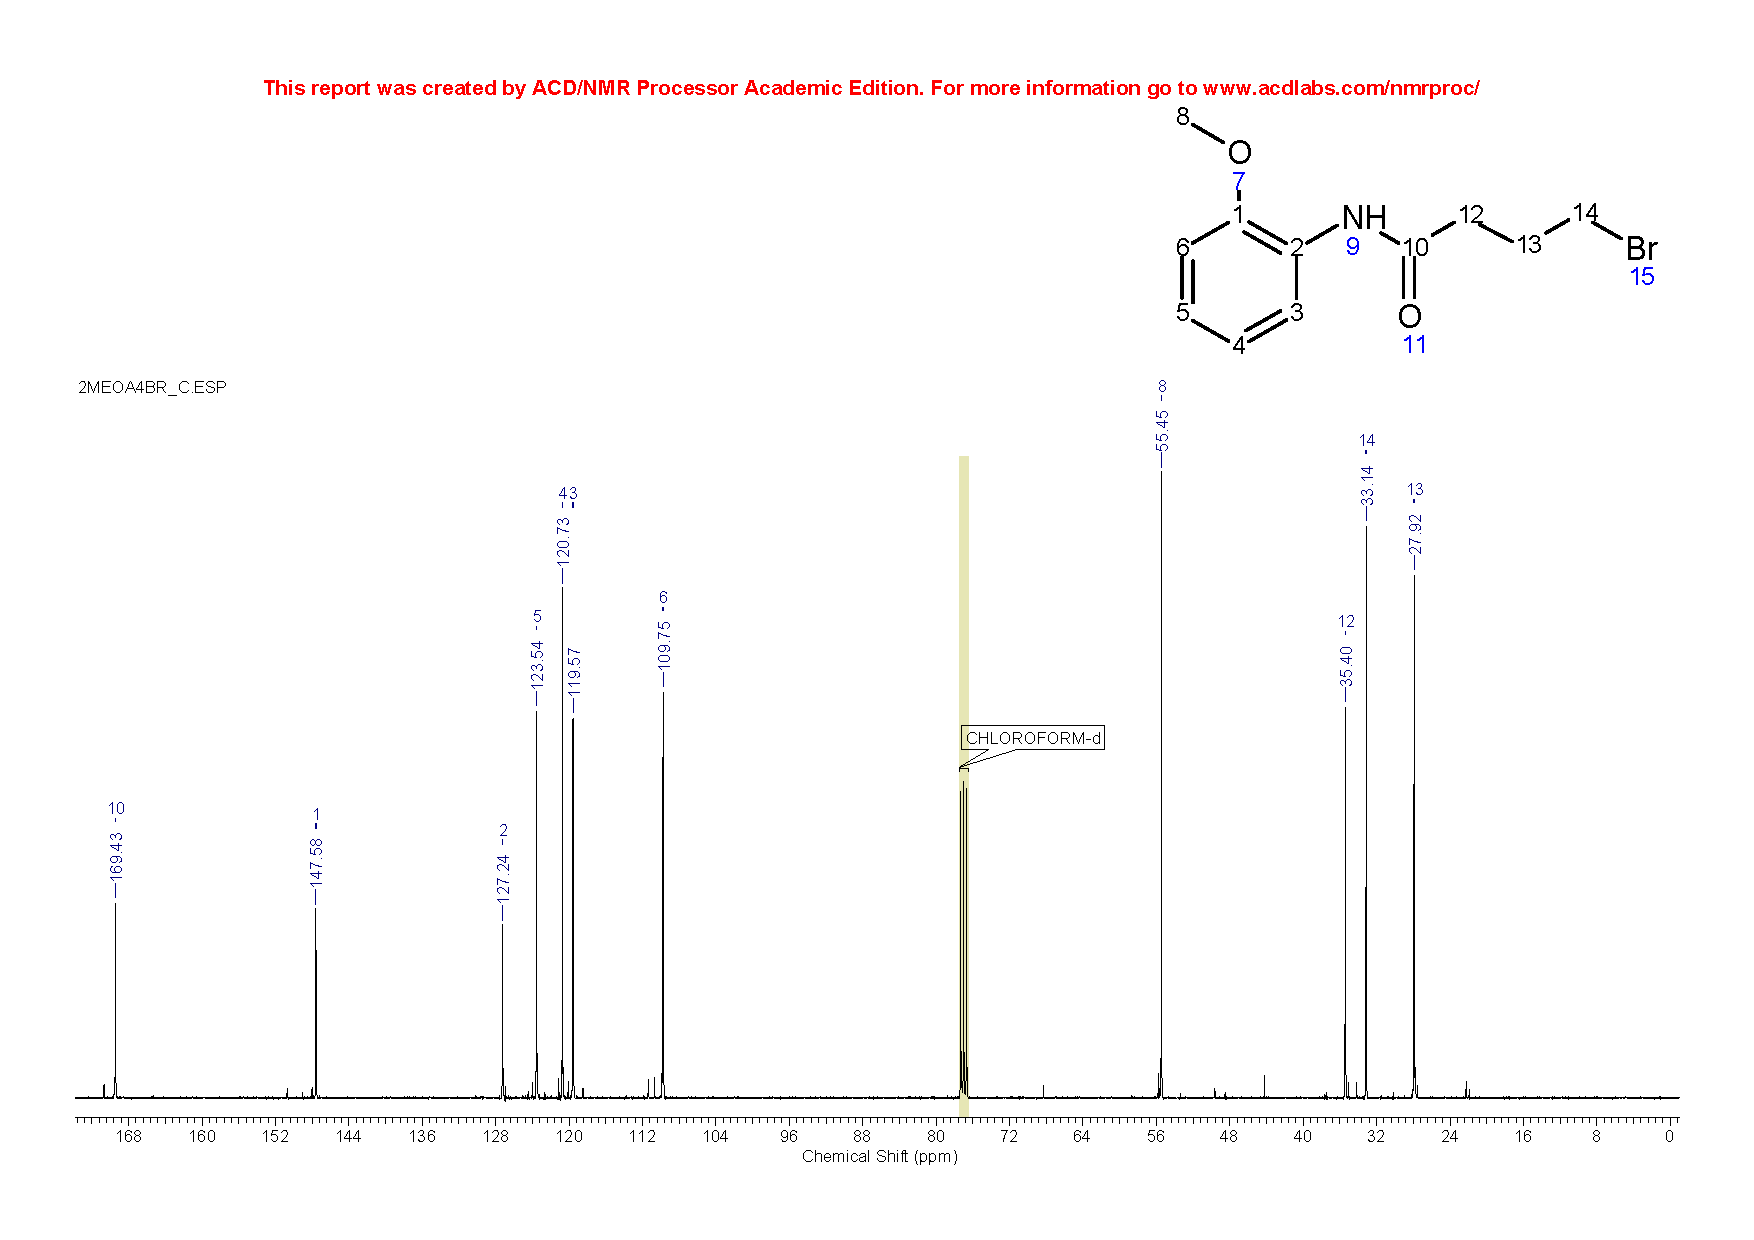
\includegraphics[ width=1.0\textwidth,height=0.43\textheight,keepaspectratio,trim={0 0 0 1.7cm},clip]{2MeOA4Br_C.pdf}
\end{figure}

\subsection{Methyl 1\hyp{}cyclopropyl\hyp{}6\hyp{}fluoro\hyp{}7\hyp{}(4\hyp{}(4\hyp{}((2\hyp{}methoxyphenyl)amino)\hyp{}4\hyp{}oxobutyl)\hyp{}piperazin\hyp{}1\hyp{}yl)\hyp{}4\hyp{}oxo\hyp{}1,4\hyp{}dihydroquinoline\hyp{}3\hyp{}carboxylate \compound{cmpd:2MeOA4CipMe}}

\begin{figure}[H]
	\centering
		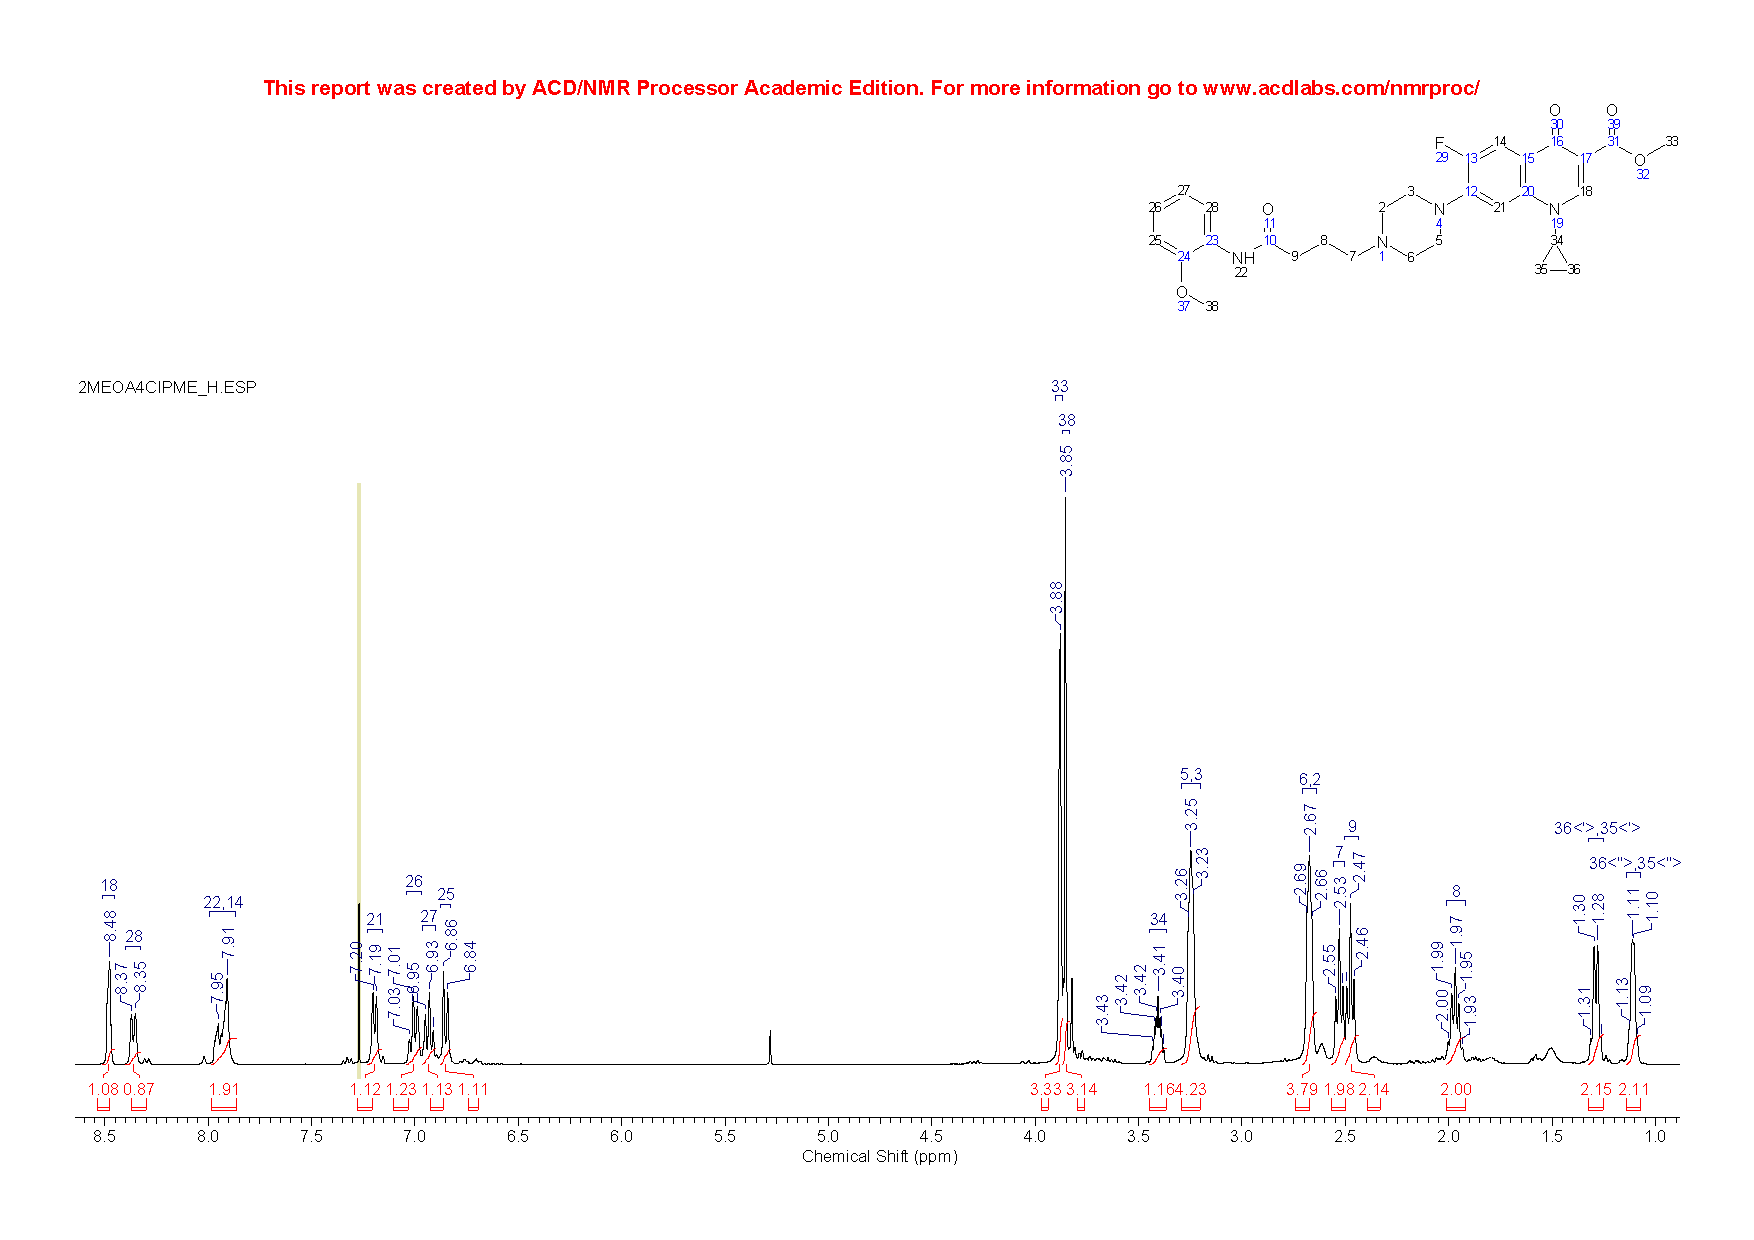
\includegraphics[ width=1.0\textwidth,height=0.43\textheight,keepaspectratio,trim={0 0 0 1.7cm},clip]{2MeOA4CipMe_H.pdf}
		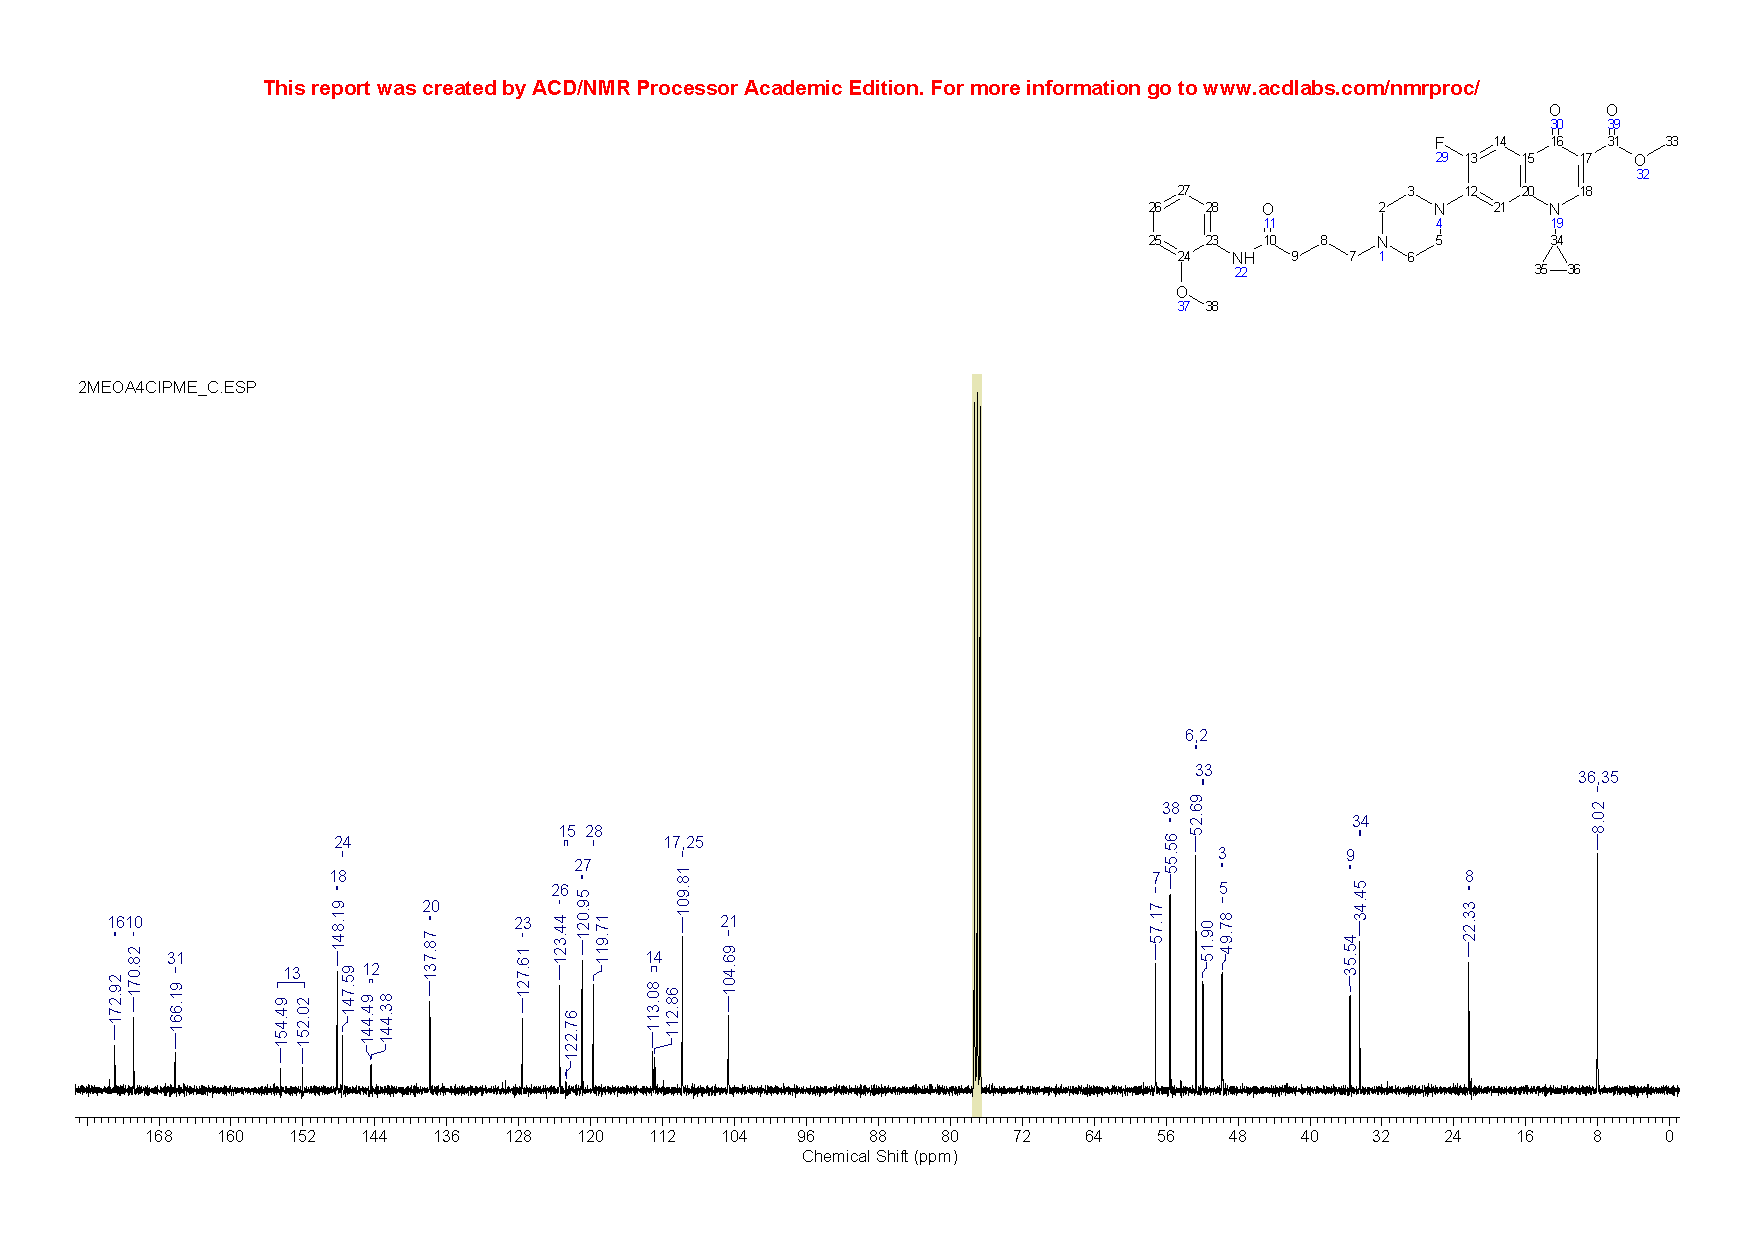
\includegraphics[ width=1.0\textwidth,height=0.43\textheight,keepaspectratio,trim={0 0 0 1.7cm},clip]{2MeOA4CipMe_C.pdf}
\end{figure}

\subsection{1\hyp{}Cyclopropyl\hyp{}6\hyp{}fluoro\hyp{}7\hyp{}(4\hyp{}(4\hyp{}(1\hyp{}(4\hyp{}((2\hyp{}methoxyphenyl)amino)\hyp{}4\hyp{}oxobutyl)\hyp{}1\textit{H}\hyp{}1,2,3\hyp{}triazol\hyp{}4\hyp{}yl)\allowbreak butyl) piperazin\hyp{}1\hyp{}yl)\hyp{}4\hyp{}oxo\hyp{}1,4\hyp{}dihydroquinoline\hyp{}3\hyp{}carboxylic acid \compound{cmpd:2MeOA4T4Cip}}

\begin{figure}[H]
	\centering
		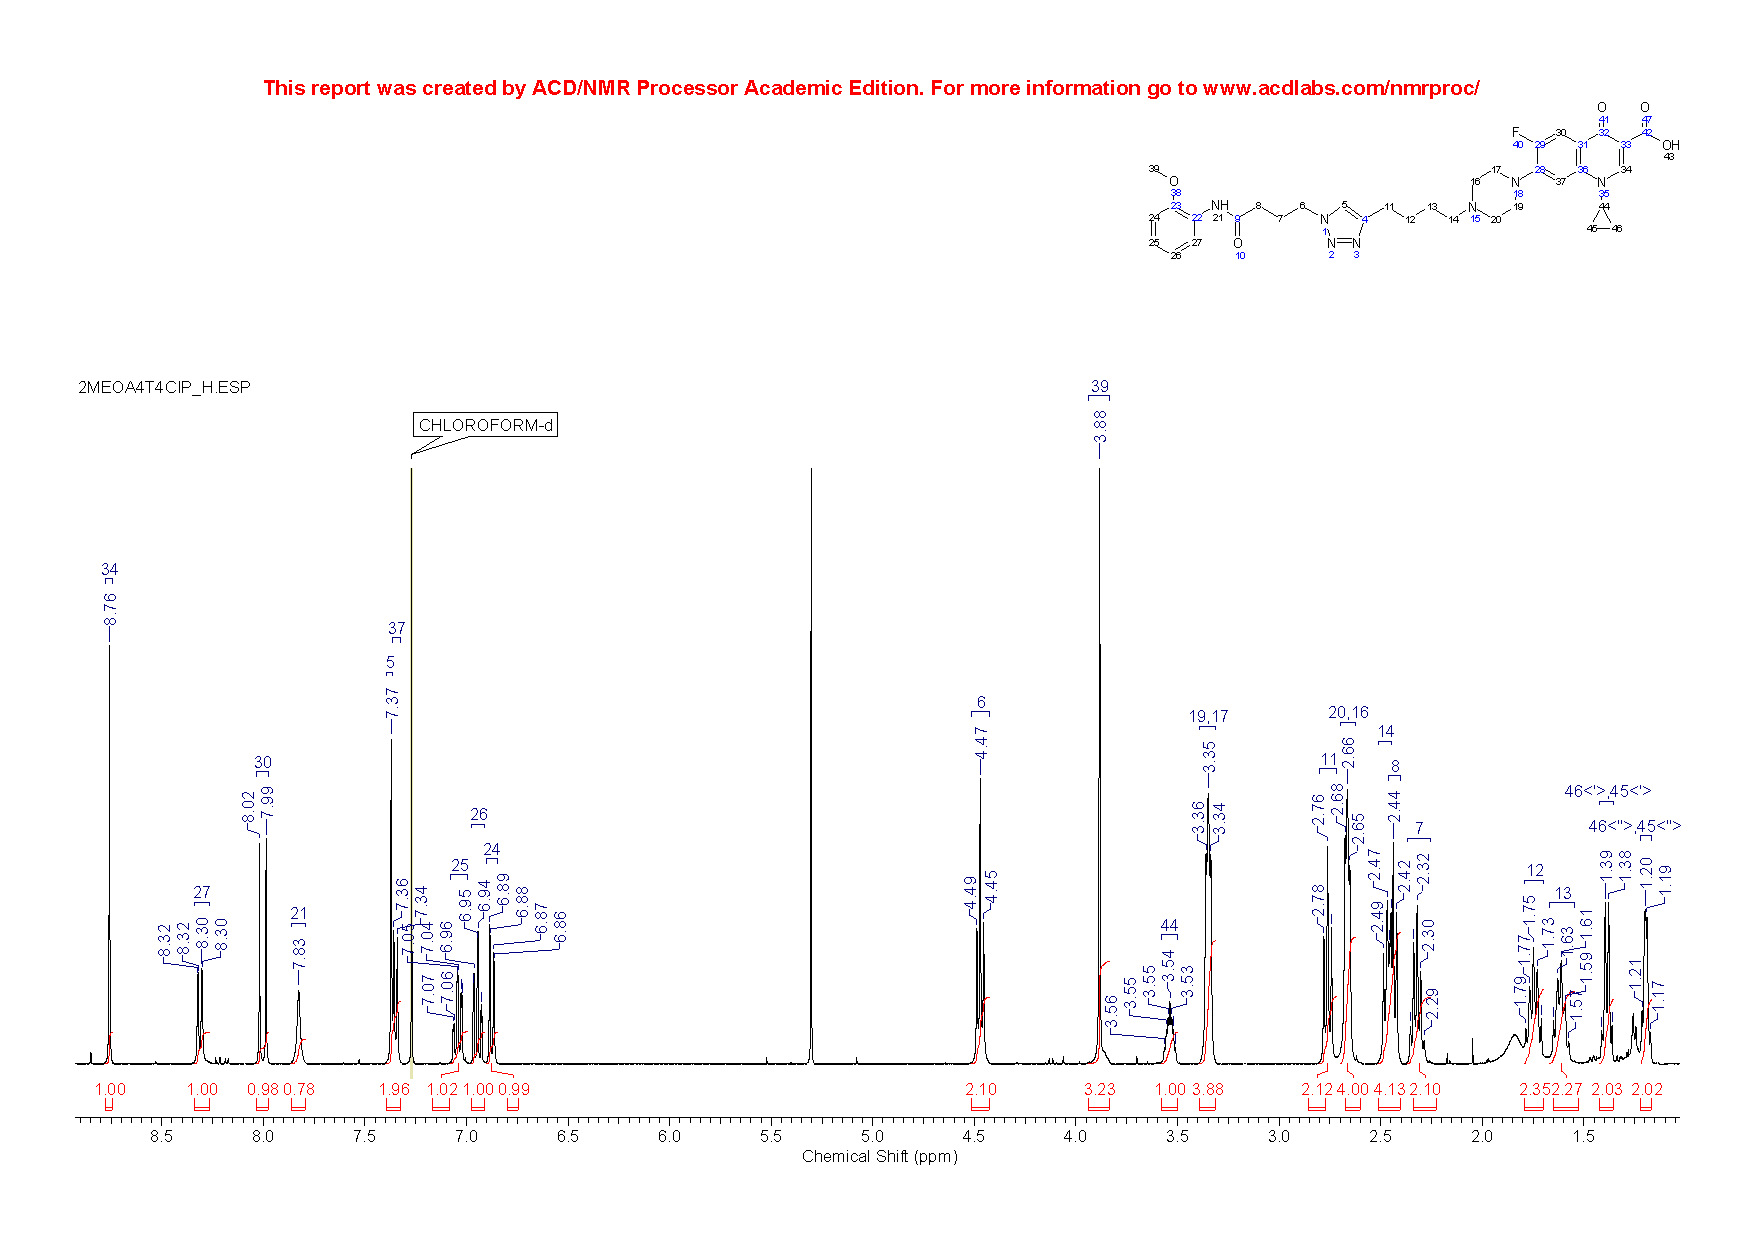
\includegraphics[ width=1.0\textwidth,height=0.43\textheight,keepaspectratio,trim={0 0 0 1.7cm},clip]{2MeOA4T4Cip_H.pdf}
		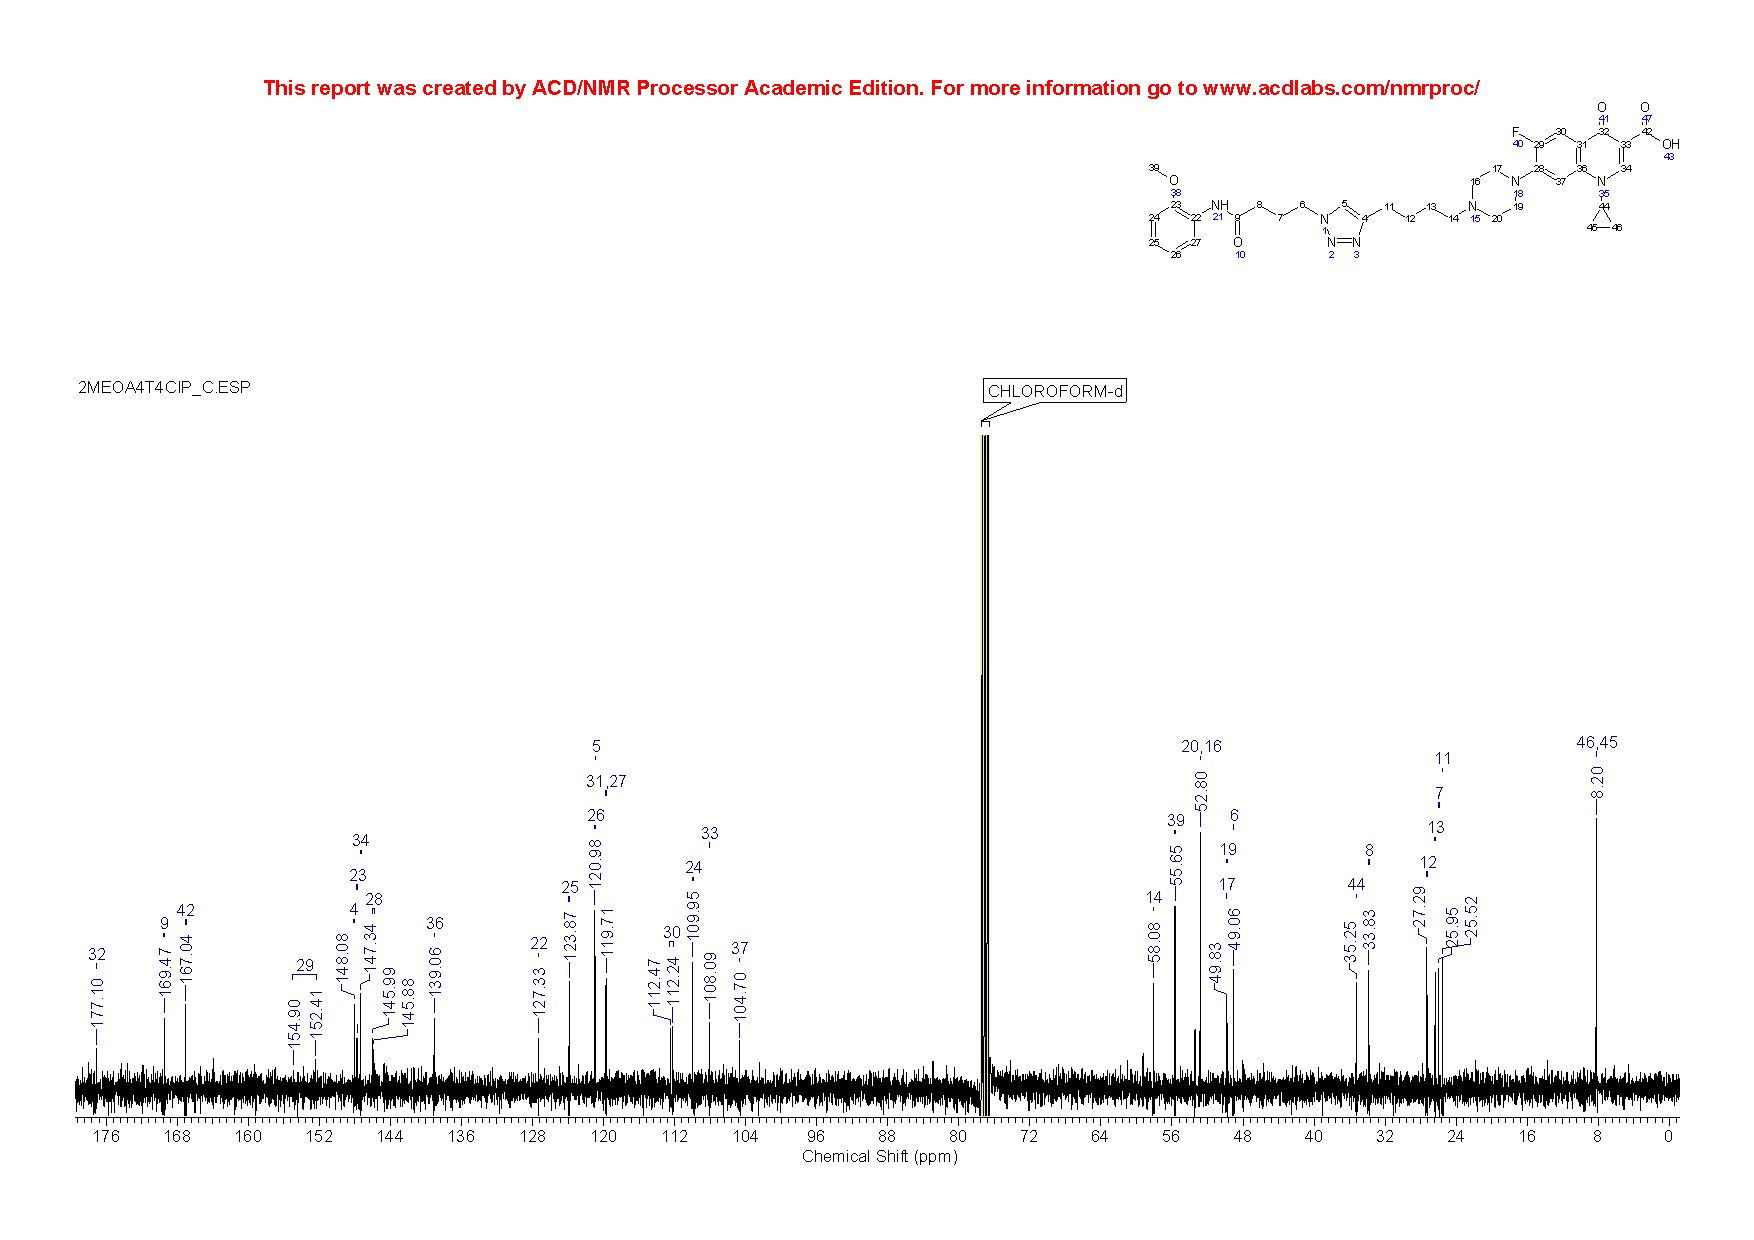
\includegraphics[ width=1.0\textwidth,height=0.43\textheight,keepaspectratio,trim={0 0 0 1.7cm},clip]{2MeOA4T4Cip_C.pdf}
\end{figure}

\subsection{4\hyp{}Bromo\hyp{}\textit{N}\hyp{}(3\hyp{}methoxyphenyl)butanamide \compound{cmpd:3MeOA4Br}}

\begin{figure}[H]
	\centering
		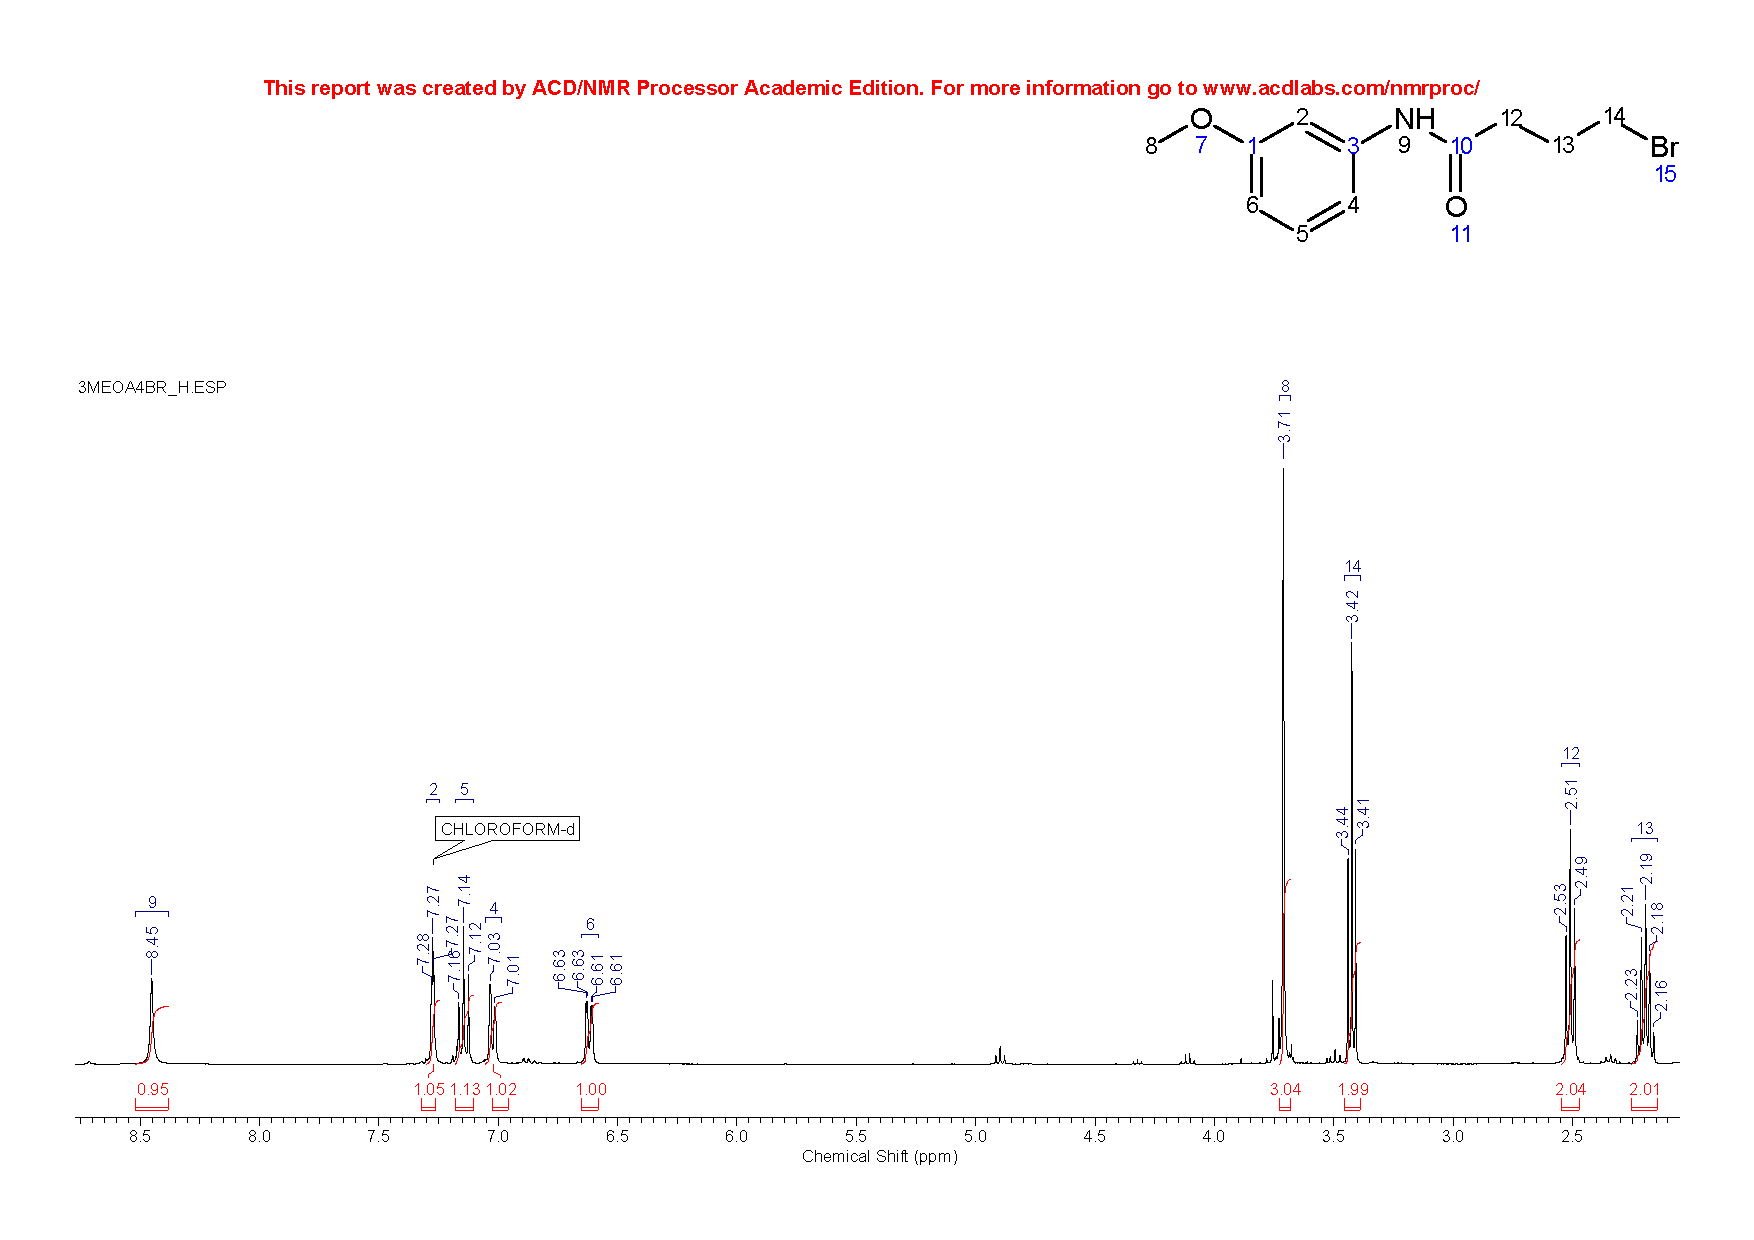
\includegraphics[ width=1.0\textwidth,height=0.43\textheight,keepaspectratio,trim={0 0 0 1.7cm},clip]{3MeOA4Br_H.pdf}
		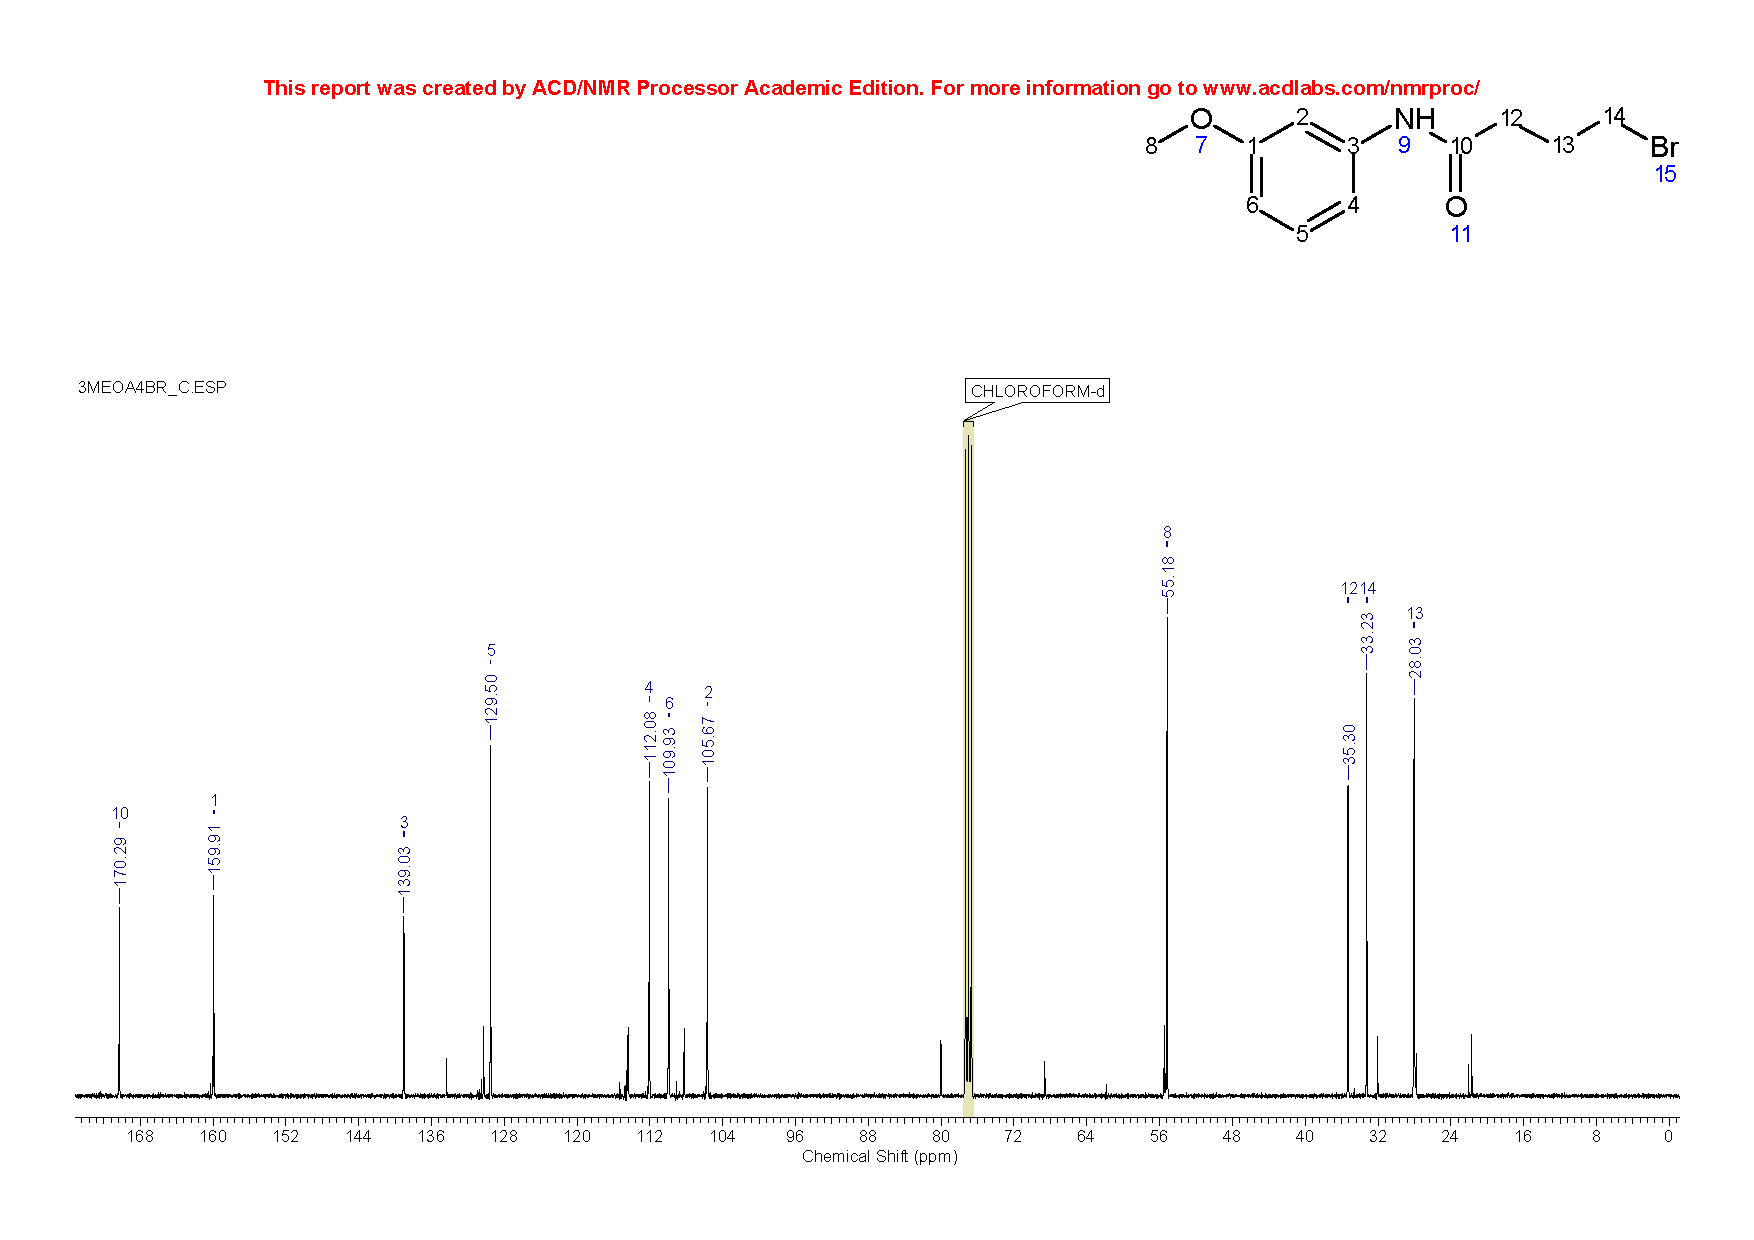
\includegraphics[ width=1.0\textwidth,height=0.43\textheight,keepaspectratio,trim={0 0 0 1.7cm},clip]{3MeOA4Br_C.pdf}
\end{figure}

\subsection{Methyl 1\hyp{}cyclopropyl\hyp{}6\hyp{}fluoro\hyp{}7\hyp{}(4\hyp{}(4\hyp{}((3\hyp{}methoxyphenyl)amino)\hyp{}4\hyp{}oxobutyl)\hyp{}piperazin\hyp{}1\hyp{}yl)\hyp{}4\hyp{}oxo\hyp{}1,4\hyp{}dihydroquinoline\hyp{}3\hyp{}carboxylate \compound{cmpd:3MeOA4CipMe}}

\begin{figure}[H]
	\centering
		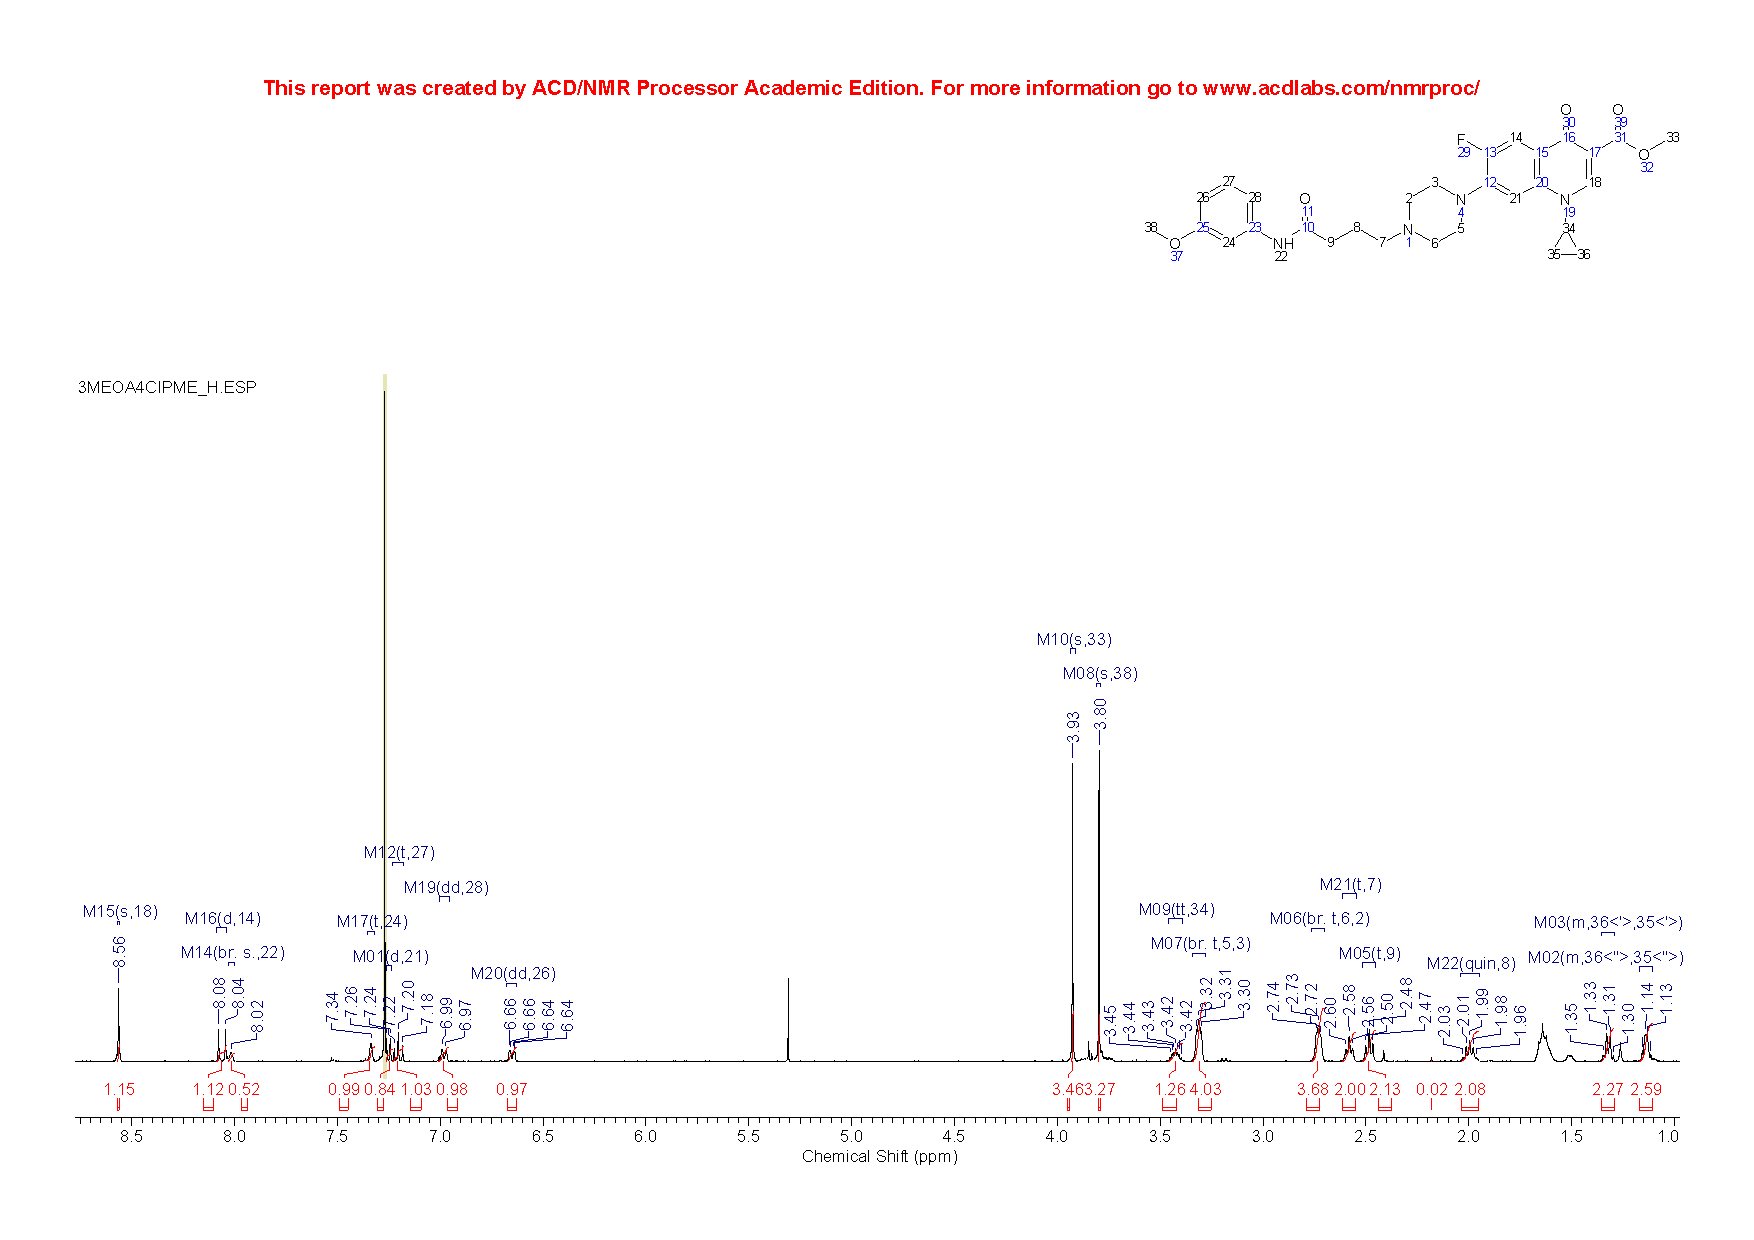
\includegraphics[ width=1.0\textwidth,height=0.43\textheight,keepaspectratio,trim={0 0 0 1.7cm},clip]{3MeOA4CipMe_H.pdf}
		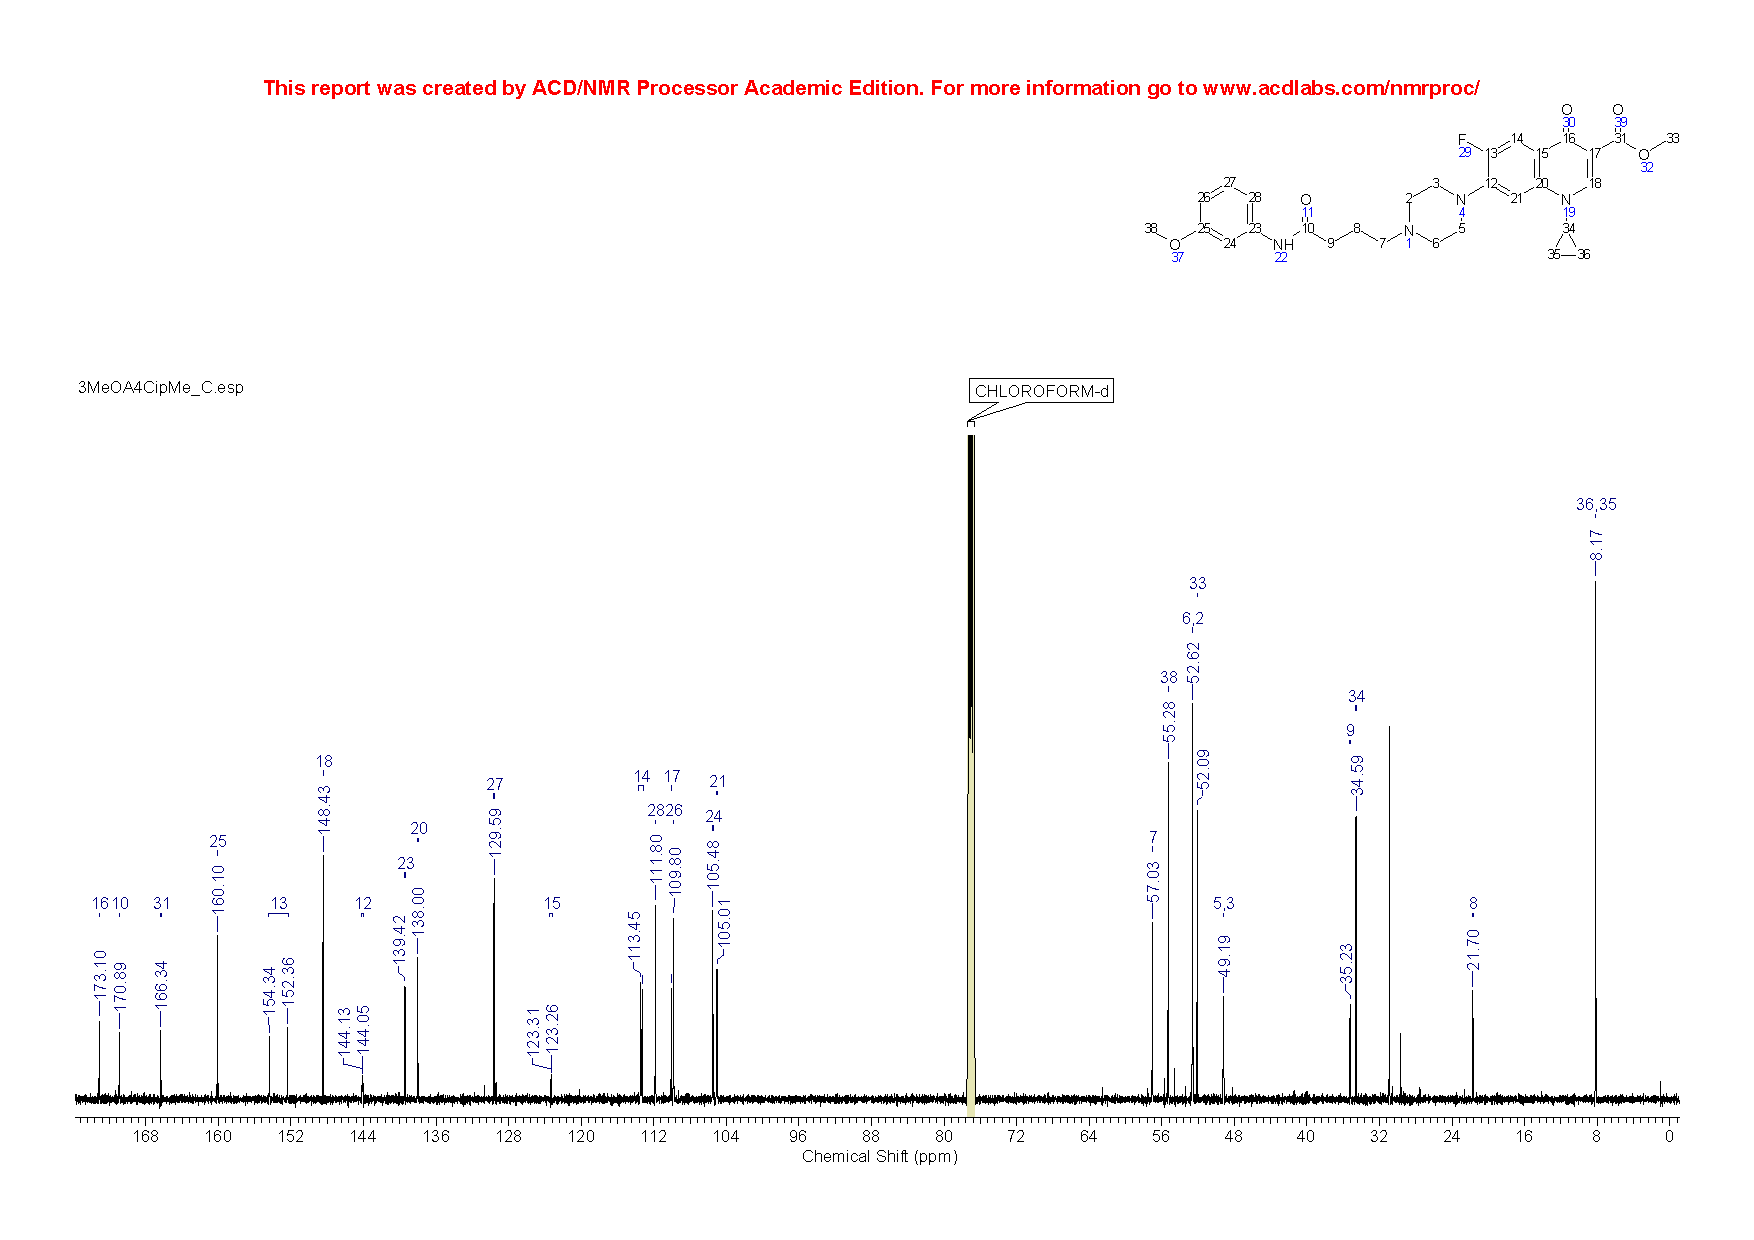
\includegraphics[ width=1.0\textwidth,height=0.43\textheight,keepaspectratio,trim={0 0 0 1.7cm},clip]{3MeOA4CipMe_C.pdf}
\end{figure}

\subsection{4\hyp{}Azido\hyp{}\textit{N}\hyp{}(3\hyp{}methoxyphenyl)butanamide \compound{cmpd:3MeOA4N3}}

\begin{figure}[H]
	\centering
		\includegraphics[ width=1.0\textwidth,height=0.43\textheight,keepaspectratio,trim={0 0 0 1.7cm},clip]{3MeOA4N3_H.pdf}
		\includegraphics[ width=1.0\textwidth,height=0.43\textheight,keepaspectratio,trim={0 0 0 1.7cm},clip]{3MeOA4N3_C.pdf}
\end{figure}

\subsection{1\hyp{}Cyclopropyl\hyp{}6\hyp{}fluoro\hyp{}7\hyp{}(4\hyp{}(4\hyp{}(1\hyp{}(4\hyp{}((3\hyp{}methoxyphenyl)amino)\hyp{}4\hyp{}oxobutyl)\hyp{}1\textit{H}\hyp{}1,2,3\hyp{}triazol\hyp{}4\hyp{}yl)\allowbreak butyl)piperazin\hyp{}1\hyp{}yl)\hyp{}4\hyp{}oxo\hyp{}1,4\hyp{}dihydroquinoline\hyp{}3\hyp{}carboxylic acid \compound{cmpd:3MeOA4T4Cip}}

\begin{figure}[H]
	\centering
		\includegraphics[ width=1.0\textwidth,height=0.43\textheight,keepaspectratio,trim={0 0 0 1.7cm},clip]{3MeOA4T4Cip_H.pdf}
		\includegraphics[ width=1.0\textwidth,height=0.43\textheight,keepaspectratio,trim={0 0 0 1.7cm},clip]{3MeOA4T4Cip_C.pdf}
\end{figure}

\subsection{4\hyp{}Azido\hyp{}\textit{N}\hyp{}((1\textit{S},2\textit{S})\hyp{}2\hyp{}hydroxycyclopentyl)butanamide \compound{cmpd:HOcy5NH4N3_SS}}

\begin{figure}[H]
	\centering
		\includegraphics[ width=1.0\textwidth,height=0.43\textheight,keepaspectratio,trim={0 0 0 1.7cm},clip]{HOcy5NH4N3_SS_H.pdf}
		\includegraphics[ width=1.0\textwidth,height=0.43\textheight,keepaspectratio,trim={0 0 0 1.7cm},clip]{HOcy5NH4N3_SS_C.pdf}
\end{figure}

\subsection{4\hyp{}Azido\hyp{}\textit{N}\hyp{}((1\textit{R},2\textit{R})\hyp{}2\hyp{}hydroxycyclopentyl)butanamide \compound{cmpd:HOcy5NH4N3_RR}} 

\begin{figure}[H]
	\centering
		\includegraphics[ width=1.0\textwidth,height=0.43\textheight,keepaspectratio,trim={0 0 0 1.7cm},clip]{HOcy5NH4N3_RR_H.pdf}
		\includegraphics[ width=1.0\textwidth,height=0.43\textheight,keepaspectratio,trim={0 0 0 1.7cm},clip]{HOcy5NH4N3_RR_C.pdf}
\end{figure}

\subsection{Methyl 1\hyp{}cyclopropyl\hyp{}6\hyp{}fluoro\hyp{}7\hyp{}(4\hyp{}(4\hyp{}(((1\textit{S},2\textit{S})\hyp{}2\hyp{}hydroxycyclopentyl)amino)\allowbreak \hyp{}4\hyp{}oxobutyl)piperazin\hyp{}1\hyp{}yl)\hyp{}4\hyp{}oxo\hyp{}1,4\hyp{}dihydroquinoline\hyp{}3\hyp{}carboxylate \compound{cmpd:HOcy5NH4CipMe_SS}}

\begin{figure}[H]
	\centering
		\includegraphics[ width=1.0\textwidth,height=0.43\textheight,keepaspectratio,trim={0 0 0 1.7cm},clip]{HOcy5NH4CipMe_SS_H.pdf}
		\includegraphics[ width=1.0\textwidth,height=0.43\textheight,keepaspectratio,trim={0 0 0 1.7cm},clip]{HOcy5NH4CipMe_SS_C.pdf}
\end{figure}

\subsection{Methyl 1\hyp{}cyclopropyl\hyp{}6\hyp{}fluoro\hyp{}7\hyp{}(4\hyp{}(4\hyp{}(((1\textit{R},2\textit{R})\hyp{}2\hyp{}hydroxycyclopentyl)amino)\allowbreak \hyp{}4\hyp{}oxobutyl)piperazin\hyp{}1\hyp{}yl)\hyp{}4\hyp{}oxo\hyp{}1,4\hyp{}dihydroquinoline\hyp{}3\hyp{}carboxylate \compound{cmpd:HOcy5NH4CipMe_RR}}

\begin{figure}[H]
	\centering
		\includegraphics[ width=1.0\textwidth,height=0.43\textheight,keepaspectratio,trim={0 0 0 1.7cm},clip]{HOcy5NH4CipMe_RR_H.pdf}
		\includegraphics[ width=1.0\textwidth,height=0.43\textheight,keepaspectratio,trim={0 0 0 1.7cm},clip]{HOcy5NH4CipMe_RR_C.pdf}
\end{figure}

\subsection{1\hyp{}Cyclopropyl\hyp{}6\hyp{}fluoro\hyp{}7\hyp{}(4\hyp{}(4\hyp{}(1\hyp{}(4\hyp{}(((1\textit{S},2\textit{S})\hyp{}2\hyp{}hydroxycyclopentyl)amino)\hyp{}4\hyp{}oxobutyl)\hyp{}1\textit{H}\hyp{}1,2,3\hyp{}triazol\hyp{}4\hyp{}yl)butyl)piperazin\hyp{}1\hyp{}yl)\hyp{}4\hyp{}oxo\hyp{}1,4\hyp{}dihydroquin\allowbreak oline\hyp{}3\hyp{}carboxylic acid \compound{cmpd:HOcy5NH4T4Cip_SS}}

\begin{figure}[H]
	\centering
		\includegraphics[ width=1.0\textwidth,height=0.43\textheight,keepaspectratio,trim={0 0 0 1.7cm},clip]{HOcy5NH4T4Cip_SS_H.pdf}
		\includegraphics[ width=1.0\textwidth,height=0.43\textheight,keepaspectratio,trim={0 0 0 1.7cm},clip]{HOcy5NH4T4Cip_SS_C.pdf}
\end{figure}

\subsection{1\hyp{}Cyclopropyl\hyp{}6\hyp{}fluoro\hyp{}7\hyp{}(4\hyp{}(4\hyp{}(1\hyp{}(4\hyp{}(((1\textit{R},2\textit{R})\hyp{}2\hyp{}hydroxycyclopentyl)amino)\hyp{}4\hyp{}oxobutyl)\hyp{}1\textit{H}\hyp{}1,2,3\hyp{}triazol\hyp{}4\hyp{}yl)butyl)piperazin\hyp{}1\hyp{}yl)\hyp{}4\hyp{}oxo\hyp{}1,4\hyp{}dihydroquin\allowbreak oline\hyp{}3\hyp{}carboxylic acid \compound{cmpd:HOcy5NH4T4Cip_RR}}

\begin{figure}[H]
	\centering
		\includegraphics[ width=1.0\textwidth,height=0.43\textheight,keepaspectratio,trim={0 0 0 1.7cm},clip]{HOcy5NH4T4Cip_RR_H.pdf}
		\includegraphics[ width=1.0\textwidth,height=0.43\textheight,keepaspectratio,trim={0 0 0 1.7cm},clip]{HOcy5NH4T4Cip_RR_C.pdf}
\end{figure}

\subsection{4\hyp{}Azido\hyp{}\textit{N}\hyp{}((1\textit{S},2\textit{S})\hyp{}2\hyp{}((\textit{tert}\hyp{}butyldimethylsilyl)oxy)cyclopentyl)butanamide \compound{cmpd:TBSOcy5NH4N3_SS}}

\begin{figure}[H]
	\centering
		\includegraphics[ width=1.0\textwidth,height=0.43\textheight,keepaspectratio,trim={0 0 0 1.7cm},clip]{TBSOcy5NH4N3_SS_H.pdf}
		\includegraphics[ width=1.0\textwidth,height=0.43\textheight,keepaspectratio,trim={0 0 0 1.7cm},clip]{TBSOcy5NH4N3_SS_C.pdf}
\end{figure}

\subsection{7\hyp{}(4\hyp{}(4\hyp{}(1\hyp{}(4\hyp{}(((1\textit{S},2\textit{S})\hyp{}2\hyp{}((\textit{tert}\hyp{}butyldimethylsilyl)oxy)cyclopentyl)amino)\hyp{}4\hyp{}oxobutyl)\hyp{}1\textit{H}\hyp{}1,2,3\hyp{}triazol\hyp{}4\hyp{}yl)butyl)piperazin\hyp{}1\hyp{}yl)\hyp{}1\hyp{}cyclopropyl\hyp{}6\hyp{}fluoro\hyp{}4\hyp{}oxo\hyp{}1,4\hyp{}dihydroquinoline\hyp{}3\hyp{}carboxylic acid \compound{cmpd:TBSOcy5NH4T4Cip_SS}}

\begin{figure}[H]
	\centering
		\includegraphics[ width=1.0\textwidth,height=0.43\textheight,keepaspectratio,trim={0 0 0 1.7cm},clip]{TBSOcy5NH4T4Cip_SS_H.pdf}
		\includegraphics[ width=1.0\textwidth,height=0.43\textheight,keepaspectratio,trim={0 0 0 1.7cm},clip]{TBSOcy5NH4T4Cip_SS_C.pdf}
\end{figure}

\subsection{4\hyp{}Chloro\hyp{}\textit{N}\hyp{}((1\textit{S},2\textit{S})\hyp{}2\hyp{}hydroxycyclopentyl)butanamide \compound{cmpd:HOcy5NH4Cl_SS}}

\begin{figure}[H]
	\centering
		\includegraphics[ width=1.0\textwidth,height=0.43\textheight,keepaspectratio,trim={0 0 0 1.7cm},clip]{HOcy5NH4Cl_SS_H.pdf}
		\includegraphics[ width=1.0\textwidth,height=0.43\textheight,keepaspectratio,trim={0 0 0 1.7cm},clip]{HOcy5NH4Cl_SS_C.pdf}
\end{figure}

\subsection{4\hyp{}Chloro\hyp{}\textit{N}\hyp{}((1\textit{R},2\textit{R})\hyp{}2\hyp{}hydroxycyclopentyl)butanamide \compound{cmpd:HOcy5NH4Cl_RR}}

\begin{figure}[H]
	\centering
		\includegraphics[ width=1.0\textwidth,height=0.43\textheight,keepaspectratio,trim={0 0 0 1.7cm},clip]{HOcy5NH4Cl_RR_H.pdf}
		\includegraphics[ width=1.0\textwidth,height=0.43\textheight,keepaspectratio,trim={0 0 0 1.7cm},clip]{HOcy5NH4Cl_RR_C.pdf}
\end{figure}

\subsection{Methyl 7\hyp{}(4\hyp{}(4\hyp{}(\textit{tert}\hyp{}butoxy)\hyp{}4\hyp{}oxobutyl)piperazin\hyp{}1\hyp{}yl)\hyp{}1\hyp{}cyclopropyl\hyp{}6\hyp{}fluoro\hyp{}4\hyp{}oxo\hyp{}1,4\hyp{}dihydroquinoline\hyp{}3\hyp{}carboxylate \compound{cmpd:tBuOO4CipMe}}

\begin{figure}[H]
	\centering
		\includegraphics[ width=1.0\textwidth,height=0.43\textheight,keepaspectratio,trim={0 0 0 1.7cm},clip]{tBuOO4CipMe_H.pdf}
		\includegraphics[ width=1.0\textwidth,height=0.43\textheight,keepaspectratio,trim={0 0 0 1.7cm},clip]{tBuOO4CipMe_C.pdf}
\end{figure}

\subsection{4\hyp{}(4\hyp{}(1\hyp{}Cyclopropyl\hyp{}6\hyp{}fluoro\hyp{}3\hyp{}(methoxycarbonyl)\hyp{}4\hyp{}oxo\hyp{}1,4\hyp{}dihydroquinolin\hyp{}7\hyp{}yl)piperazin\hyp{}1\hyp{}yl)bu\allowbreak tanoic acid, trifluoroacetic acid salt \compound{cmpd:HOO4CipMeTFA}}

\begin{figure}[H]
	\centering
		\includegraphics[ width=1.0\textwidth,height=0.43\textheight,keepaspectratio,trim={0 0 0 1.7cm},clip]{HOO4CipMeTFA_H.pdf}
		\includegraphics[ width=1.0\textwidth,height=0.43\textheight,keepaspectratio,trim={0 0 0 1.7cm},clip]{HOO4CipMeTFA_C.pdf}
\end{figure}









%\subsection{Methyl (\textit{S})\hyp{}1\hyp{}cyclopropyl\hyp{}6\hyp{}fluoro\hyp{}4\hyp{}oxo\hyp{}7\hyp{}(4\hyp{}(4\hyp{}oxo\hyp{}4\hyp{}((2\hyp{}oxocyclopentyl)am\hyp{}ino)butyl)piperazin\hyp{}1\hyp{}yl)\hyp{}1,4\hyp{}dihydroquinoline\hyp{}3\hyp{}carboxylate \compound{cmpd:Ocy5NH4CipMe(S)}}
%
%\begin{figure}[H]
%	\centering
%		\includegraphics[ width=1.0\textwidth,height=0.43\textheight,keepaspectratio,trim={0 0 0 1.7cm},clip]{Ocy5NH4CipMe_S_H.pdf}
%		\includegraphics[ width=1.0\textwidth,height=0.43\textheight,keepaspectratio,trim={0 0 0 1.7cm},clip]{Ocy5NH4CipMe_S_C.pdf}
%\end{figure}


\subsection{Methyl 1\hyp{}cyclopropyl\hyp{}6\hyp{}fluoro\hyp{}7\hyp{}(4\hyp{}(4\hyp{}(((\textit{trans})\hyp{}2\hyp{}hydroxycyclohexyl)amino)\hyp{}4\hyp{}oxobutyl)piperazin\hyp{}1\hyp{}yl)\hyp{}4\hyp{}oxo\hyp{}1,4\hyp{}dihydroquinoline\hyp{}3\hyp{}carboxylate \compound{cmpd:HOcy6NH4CipMe}}

\begin{figure}[H]
	\centering
		\includegraphics[ width=1.0\textwidth,height=0.43\textheight,keepaspectratio,trim={0 0 0 1.7cm},clip]{HOcy6NH4CipMe_H.pdf}
		\includegraphics[ width=1.0\textwidth,height=0.43\textheight,keepaspectratio,trim={0 0 0 1.7cm},clip]{HOcy6NH4CipMe_C.pdf}
\end{figure}

\subsection{Methyl 1\hyp{}cyclopropyl\hyp{}6\hyp{}fluoro\hyp{}4\hyp{}oxo\hyp{}7\hyp{}(4\hyp{}(4\hyp{}oxo\hyp{}4\hyp{}((2\hyp{}oxocyclohexyl)amino)\hyp{}butyl)piperazin\hyp{}1\hyp{}yl)\hyp{}1,4\hyp{}dihydroquinoline\hyp{}3\hyp{}carboxylate \compound{cmpd:Ocy6NH4CipMe}}

\begin{figure}[H]
	\centering
		\includegraphics[ width=1.0\textwidth,height=0.43\textheight,keepaspectratio,trim={0 0 0 1.7cm},clip]{Ocy6NH4CipMe_H.pdf}
		\includegraphics[ width=1.0\textwidth,height=0.43\textheight,keepaspectratio,trim={0 0 0 1.7cm},clip]{Ocy6NH4CipMe_C.pdf}
\end{figure}


\subsection{4\hyp{}Chloro\hyp{}\textit{N}\hyp{}((\textit{trans})\hyp{}2\hyp{}hydroxycyclohexyl)butanamide  \compound{cmpd:HOcy6NH4Cl}}

\begin{figure}[H]
	\centering
		\includegraphics[ width=1.0\textwidth,height=0.43\textheight,keepaspectratio,trim={0 0 0 1.7cm},clip]{HOcy6NH4Cl_H.pdf}
		\includegraphics[ width=1.0\textwidth,height=0.43\textheight,keepaspectratio,trim={0 0 0 1.7cm},clip]{HOcy6NH4Cl_C.pdf}
\end{figure}

\subsection{4\hyp{}Azido\hyp{}\textit{N}\hyp{}((\textit{trans})\hyp{}2\hyp{}hydroxycyclohexyl)butanamide  \compound{cmpd:HOcy6NH4N3}}

\begin{figure}[H]
	\centering
		\includegraphics[ width=1.0\textwidth,height=0.43\textheight,keepaspectratio,trim={0 0 0 1.7cm},clip]{HOcy6NH4N3_H.pdf}
		\includegraphics[ width=1.0\textwidth,height=0.43\textheight,keepaspectratio,trim={0 0 0 1.7cm},clip]{HOcy6NH4N3_C.pdf}
\end{figure}



\subsection{1\hyp{}Cyclopropyl\hyp{}6\hyp{}fluoro\hyp{}7\hyp{}(4\hyp{}(4\hyp{}(1\hyp{}(4\hyp{}(((\textit{trans})\hyp{}2\hyp{}hydroxycyclohexyl)amino)\hyp{}4\hyp{}oxobutyl)\hyp{}1\textit{H}\hyp{}1,2,3\hyp{}triazol\hyp{}4\hyp{}yl)butyl)piperazin\hyp{}1\hyp{}yl)\hyp{}4\hyp{}oxo\hyp{}1,4\hyp{}dihydroquinoline\hyp{}3\hyp{}carboxylic acid \compound{cmpd:HOcy6NH4T4Cip}}

\begin{figure}[H]
	\centering
		\includegraphics[ width=1.0\textwidth,height=0.43\textheight,keepaspectratio,trim={0 0 0 1.7cm},clip]{HOcy6NH4T4Cip_H.pdf}
		\includegraphics[ width=1.0\textwidth,height=0.43\textheight,keepaspectratio,trim={0 0 0 1.7cm},clip]{HOcy6NH4T4Cip_C.pdf}
\end{figure}

\subsection{1\hyp{}Cyclopropyl\hyp{}6\hyp{}fluoro\hyp{}4\hyp{}oxo\hyp{}7\hyp{}(4\hyp{}(4\hyp{}(1\hyp{}(4\hyp{}oxo\hyp{}4\hyp{}((2\hyp{}oxocyclohexyl)amino)but\allowbreak yl)\hyp{}1\textit{H}\hyp{}1,2,3\hyp{}triazol\hyp{}4\hyp{}yl)butyl)piperazin\hyp{}1\hyp{}yl)\hyp{}1,4\hyp{}dihydroquinoline\hyp{}3\hyp{}carboxy\allowbreak lic acid \compound{cmpd:Ocy6NH4T4Cip}}

\begin{figure}[H]
	\centering
		\includegraphics[ width=1.0\textwidth,height=0.43\textheight,keepaspectratio,trim={0 0 0 1.7cm},clip]{Ocy6NH4T4Cip_H.pdf}
		\includegraphics[ width=1.0\textwidth,height=0.43\textheight,keepaspectratio,trim={0 0 0 1.7cm},clip]{Ocy6NH4T4Cip_C.pdf}
\end{figure}
